\documentclass[11pt]{article}

% ---------- Packages ----------
\usepackage[margin=1in]{geometry}
\usepackage{graphicx}
\usepackage{grffile}          % filenames containing dots (M1-3.6-01-...)
\usepackage{booktabs}
\usepackage{longtable}
\usepackage{array}

% fraction-of-textwidth ragged-right column; subtracts its own
% intercolumn padding so the fractions can simply sum to 1.0
\newcolumntype{R}[1]{%
  >{\raggedright\arraybackslash}p{\dimexpr#1\textwidth-2\tabcolsep\relax}}
\usepackage{xcolor}
\usepackage{listings}
\usepackage{hyperref}
\usepackage{caption}
\usepackage{float}
\usepackage{enumitem}
\usepackage{fancyhdr}
\usepackage{parskip}
\usepackage{url}
\usepackage[protrusion=true,expansion=false]{microtype} % expansion off: bitmap tt fonts

% ---------- Line breaking in long \texttt{} paths ----------
% Paths like user/llama_core.c are a single unbreakable word to TeX and
% overhang the margin. Give the paragraph builder room, and make the
% punctuation inside typewriter text a legal breakpoint.
\emergencystretch=3em
\let\origunderscore\_
\renewcommand{\_}{\origunderscore\allowbreak}


% ---------- Where the images live ----------
\graphicspath{{Figures/}{Screenshots/}}

\hypersetup{
    colorlinks=true,
    linkcolor=blue,
    urlcolor=blue,
    citecolor=blue
}

\pagestyle{fancy}
\fancyhf{}
\fancyhead[L]{CSE331 Operating Systems --- Milestone 1}
\fancyhead[R]{\thepage}
\renewcommand{\headrulewidth}{0.4pt}

% ---------- Code / transcript listing style ----------
\lstdefinestyle{shell}{
    basicstyle=\ttfamily\footnotesize,
    backgroundcolor=\color{black!5},
    frame=single,
    breaklines=true,
    columns=fullflexible,
    keepspaces=true
}
\lstdefinestyle{mermaid}{
    basicstyle=\ttfamily\footnotesize,
    backgroundcolor=\color{blue!4},
    frame=single,
    breaklines=true,
    columns=fullflexible,
    keepspaces=true,
    language={},
}
\lstset{style=shell}

\title{\textbf{Distributed Inference on xv6}\\[4pt]
\large Milestone 1: Understand and Characterise}

\date{CSE331 Operating Systems \\ \today}

\begin{document}

\maketitle
\thispagestyle{empty}

\newpage
\tableofcontents
\newpage

% =====================================================================
\section*{Team Information}
\addcontentsline{toc}{section}{Team Information}
% =====================================================================

\begin{table}[H]
\centering
\begin{tabular}{@{}llp{7.2cm}@{}}
\toprule
\textbf{Name} & \textbf{ERP ID} & \textbf{Contribution} \\
\midrule
Ahsan Haris (Group Lead) & 30485 & Repository administration, coordination, review \\
Ahmed Abdul Rahim & 30609 & Runbook (\S3.2), bring-up transcripts, reverse-engineering workflow, baseline timings, figures F0--F7 \\
Aliya Fatima & 31724 & Architecture map, system-call table, report drafting \\
Bareera Rehan & 30696 & Hardware counter measurements under the debugger, observations log \\
\bottomrule
\end{tabular}
\caption{Team members, ERP IDs, and division of work.}
\end{table}

\noindent\textbf{Repository link:} \url{https://github.com/aliyafatima001100-pixel/xv6_llm_runtime}

\vspace{6pt}
\noindent\textbf{Platform.} Every measurement, transcript and screenshot in this
report was produced on one machine: WSL2 Ubuntu 24.04 on Windows, QEMU 8.2.2,
GNU objdump 2.42 (\texttt{riscv64-unknown-elf}), GDB 15.1 (multiarch). All
figures are in \texttt{Figures/} and all console screenshots in
\texttt{Screenshots/}, both beside this document.
The counter totals in Table~\ref{tab:baseline-counters} are the one exception: those three runs were taken by a second team member on a separate machine. The validation run in Table~\ref{tab:counter-validation} and Figure~\ref{fig:counters-gdb} was taken on the machine described above.

% =====================================================================
\section*{3.0 Warm-Up: Reconstruct a Call Graph from a Binary}
\addcontentsline{toc}{section}{3.0 Warm-Up: Reconstruct a Call Graph from a Binary}

\subsection*{A. Method / Reverse-Engineering Workflow}
The call graph was reconstructed directly from the precompiled RISC-V binary \texttt{warmup/\allowbreak{}build/\allowbreak{}challenge} without access to the original source code. \texttt{nm} was used first to enumerate the text-segment symbols and their addresses, which bounds each function to an address range and fixes the universe of functions \texttt{compute} could possibly reach. The \texttt{objdump} disassembler was then used statically to inspect the functions reached from \texttt{compute}. Each \texttt{jal} instruction was treated as a function call, and its target address was matched with the corresponding function symbol to map out all call edges. No dynamic tracing was required: the intact symbol table is what makes each \texttt{jal} operand resolvable back to a name.

\begin{figure}[H]
\centering
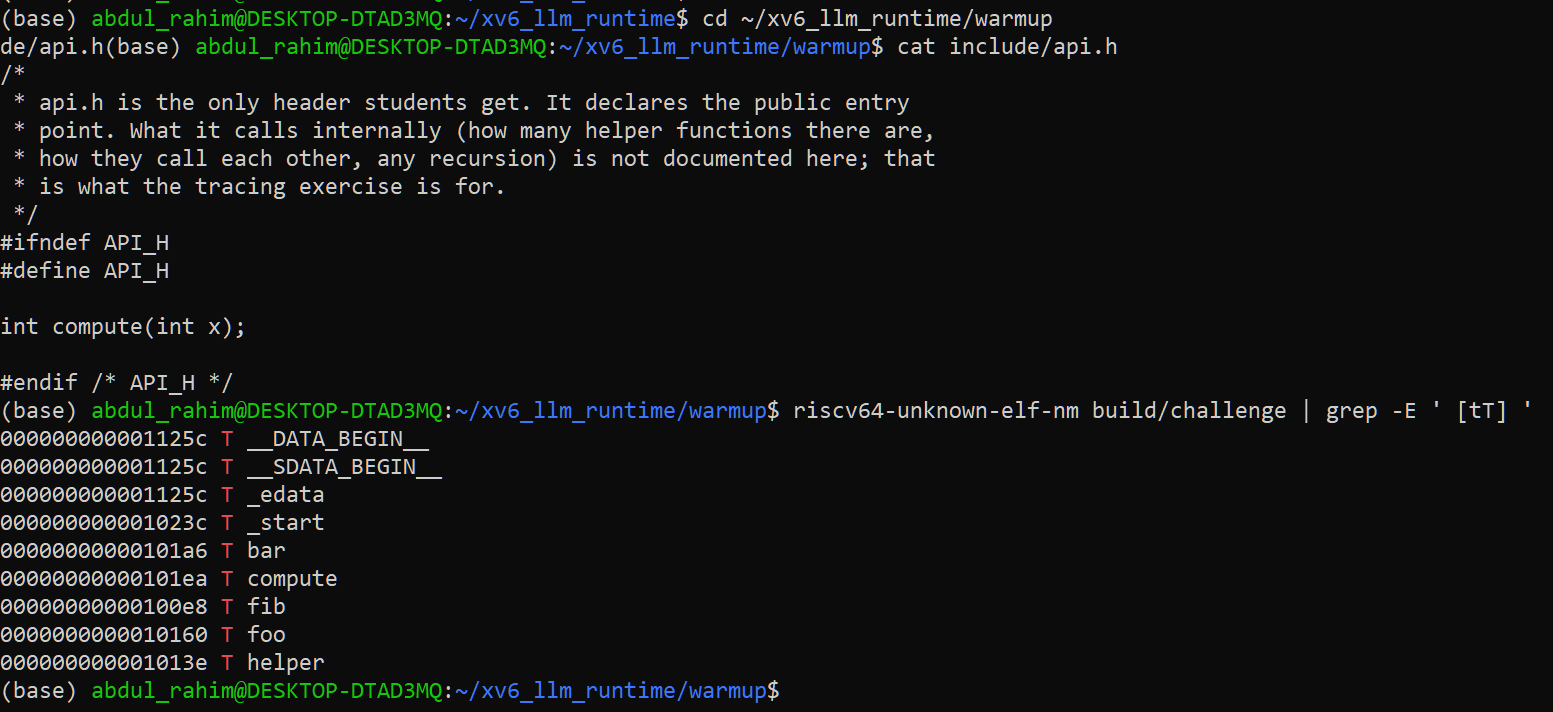
\includegraphics[width=0.72\textwidth]{M1-3.0-01-nm-challenge.png}
\caption{\texttt{nm} output for \texttt{build/challenge}. Five real functions --- \texttt{fib} at \texttt{0x100e8}, \texttt{helper} at \texttt{0x1013e}, \texttt{foo} at \texttt{0x10160}, \texttt{bar} at \texttt{0x101a6}, \texttt{compute} at \texttt{0x101ea} --- plus \texttt{\_start} and three linker markers.}
\label{fig:nm-challenge}
\end{figure}

\subsection*{B. Disassembly Evidence}
The following essential \texttt{jal} instructions were extracted from the \texttt{objdump} output to verify the call edges:

\textbf{1. \texttt{compute}:}
\begin{lstlisting}
101fe:    jal    10160 <foo>
1021a:    jal    101a6 <bar>
\end{lstlisting}

\textbf{2. \texttt{foo}:}
\begin{lstlisting}
10174:    jal    1013e <helper>
1018e:    jal    100e8 <fib>
\end{lstlisting}

\textbf{3. \texttt{bar}:}
\begin{lstlisting}
101c4:    jal    10160 <foo>
101d2:    jal    10160 <foo>
\end{lstlisting}

\textbf{4. \texttt{fib}:}
\begin{lstlisting}
00000000000100e8 <fib>:
...
10116:    jal    100e8 <fib>
10128:    jal    100e8 <fib>
\end{lstlisting}

\begin{figure}[H]
\centering
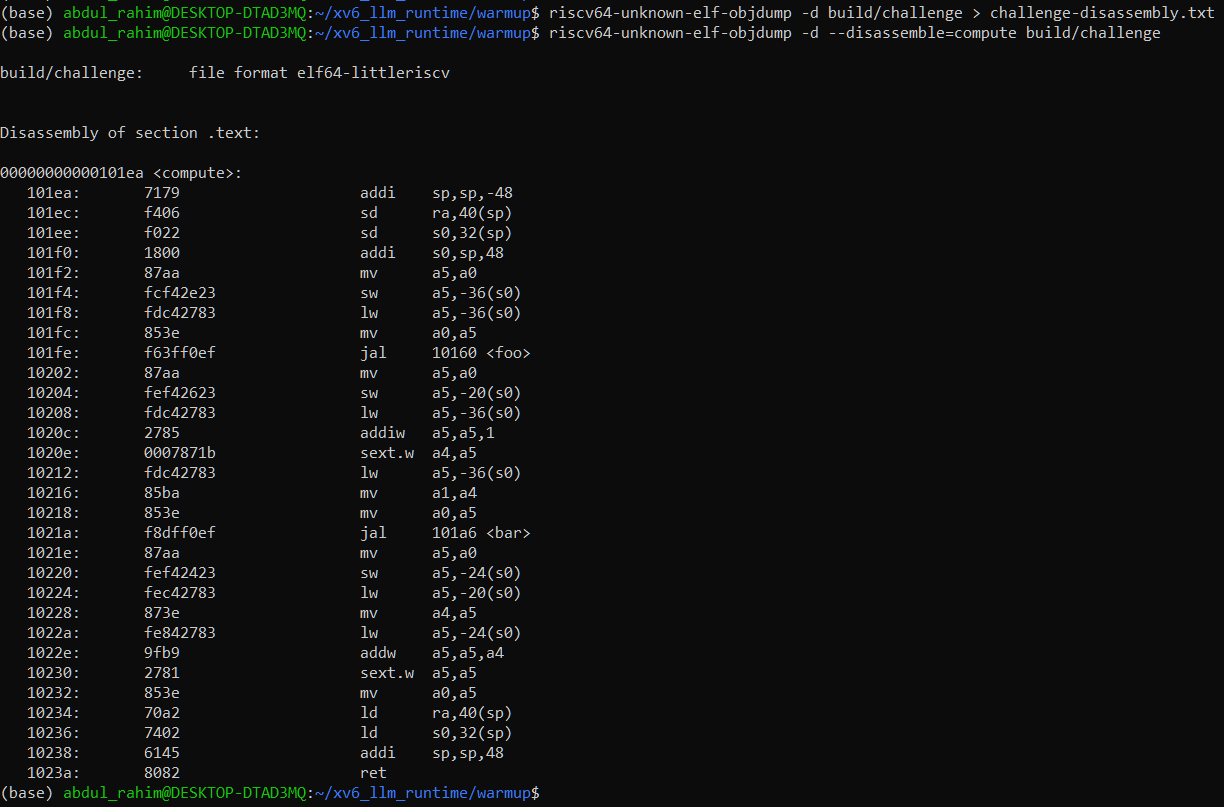
\includegraphics[width=0.72\textwidth]{M1-3.0-02-disas-compute.png}
\caption{Disassembly of \texttt{compute}. Its only two \texttt{jal} instructions target \texttt{0x10160} (\texttt{foo}) and \texttt{0x101a6} (\texttt{bar}); everything else is arithmetic and stack management.}
\label{fig:disas-compute}
\end{figure}

\begin{figure}[H]
\centering
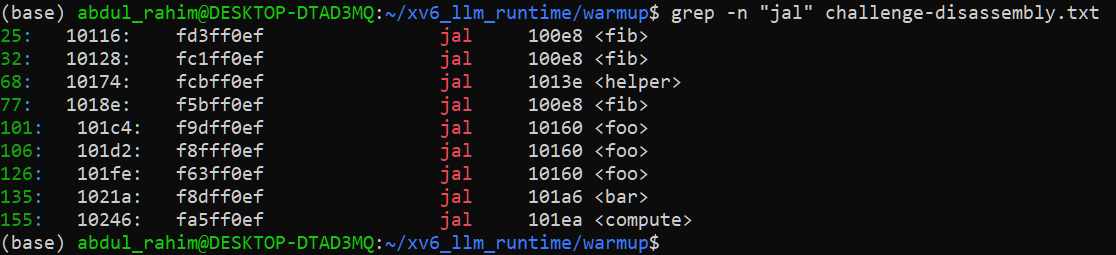
\includegraphics[width=0.94\textwidth]{M1-3.0-03-all-jal-edges.png}
\caption{All nine call sites in the binary, obtained by grepping the full disassembly for \texttt{jal}. Attributing each address to the function whose range contains it produces the complete edge set.}
\label{fig:jal-edges}
\end{figure}

\subsection*{C. Call Graph}

The following Mermaid flowchart was reconstructed directly from the
\texttt{jal} targets identified in the disassembly above.

\begin{lstlisting}[style=mermaid]
flowchart TD
    compute --> foo
    compute --> bar
    bar --> foo
    foo --> helper
    foo --> fib
    fib --> fib
\end{lstlisting}

\begin{figure}[H]
    \centering
    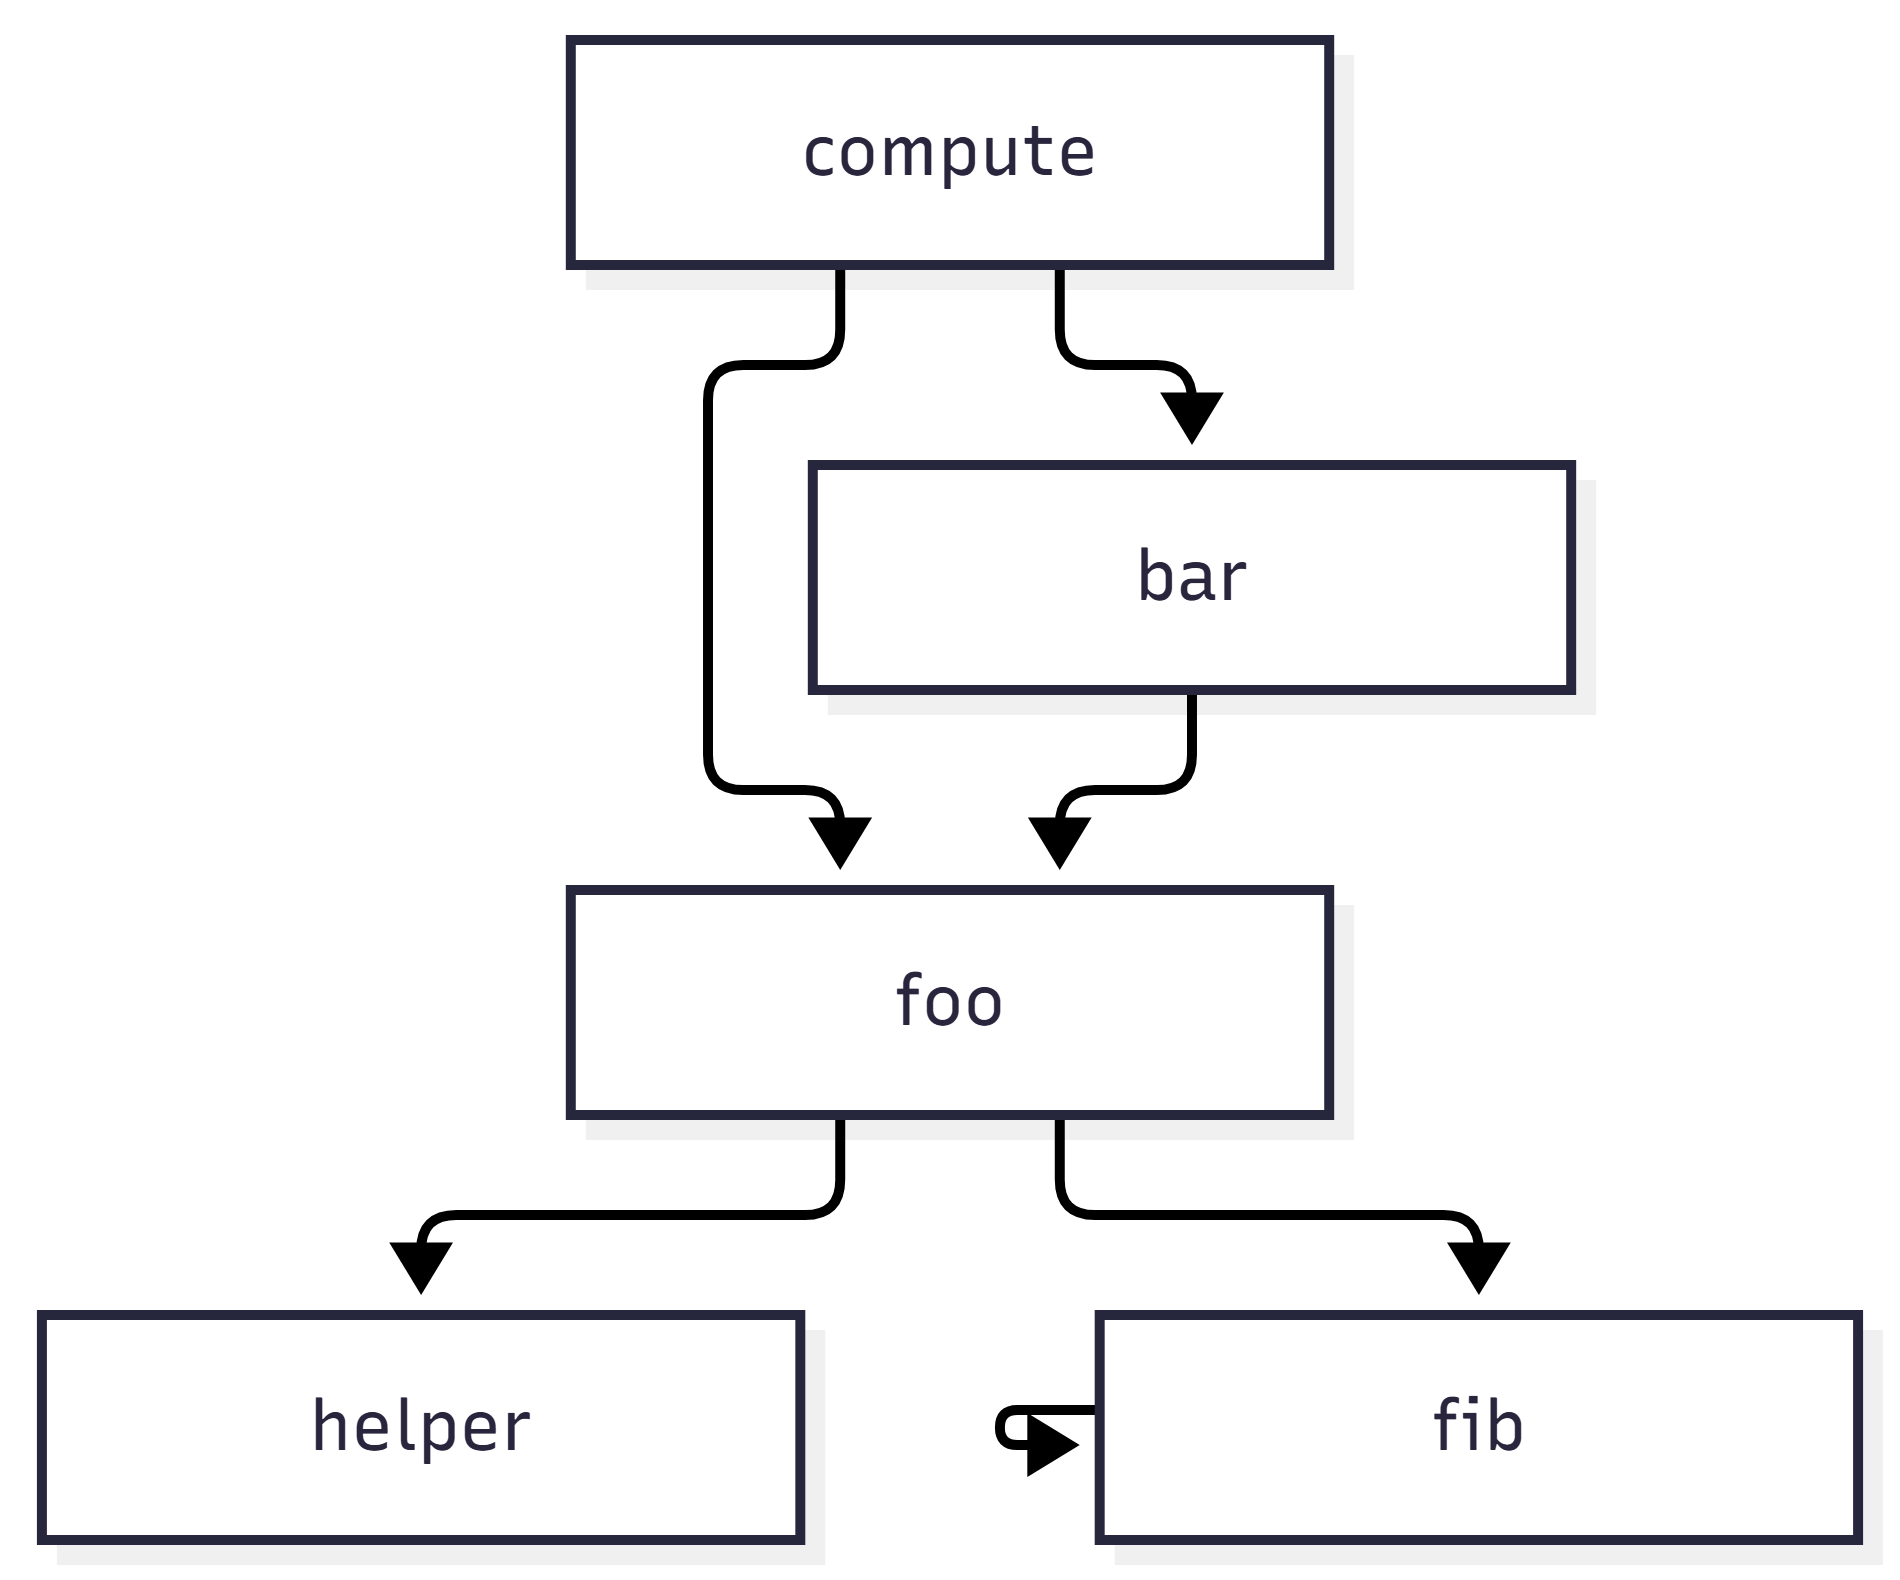
\includegraphics[width=0.42\textwidth]{F0-warmup-callgraph.png}
    \caption{F0: Call graph reconstructed statically from the
    disassembled binary, rooted at \texttt{compute}.}
    \label{fig:callgraph}
\end{figure}

\subsection*{D. Findings}
To establish the final facts, the call graph was verified through a unified walkthrough: the complete graph (\texttt{compute} $\rightarrow$ \texttt{foo}, \texttt{compute} $\rightarrow$ \texttt{bar}, \texttt{foo} $\rightarrow$ \texttt{helper}, \texttt{foo} $\rightarrow$ \texttt{fib}, \texttt{bar} $\rightarrow$ \texttt{foo}, and \texttt{fib} $\rightarrow$ \texttt{fib}) was validated by mapping every encountered \texttt{jal} target address back to its respective symbol. Furthermore, \texttt{fib} was definitively identified as recursive because its disassembly contains direct \texttt{jal} instructions targeting its own entry address (\texttt{0x100e8}), and \texttt{foo} was identified as having multiple callers because static inspection shows two distinct callers (\texttt{compute} and \texttt{bar}), with \texttt{bar} containing two separate call sites targeting \texttt{foo}.

\texttt{fib} also has two distinct callers (\texttt{foo} and itself), but one of those is its own recursion, so \texttt{foo} is the unambiguous answer to the third question.

\subsection*{E. Kernel Entry-Point Trace}
\textbf{Selected kernel entry point:} \texttt{sys\_exec}

\begin{lstlisting}
(gdb) target remote localhost:26000
Remote debugging using localhost:26000
0x0000000000001000 in ?? ()
(gdb) break sys_exec
Breakpoint 1 at 0x80005856
(gdb) continue
Continuing.

Breakpoint 1, 0x0000000080005856 in sys_exec ()
(gdb) backtrace
#0  0x0000000080005856 in sys_exec ()
#1  0x00000000800014dc in syscall ()
#2  0x0000000080001224 in usertrap ()
#3  0x0000003ffffff124 in ?? ()
(gdb) info registers a0 a1 a2
a0             0x1      1
a1             0x3fffffbdf8     274877890040
a2             0x1      1
(gdb) info registers sp s0
sp             0x3fffffbdf0     0x3fffffbdf0
s0             0x3fffffbfc0     0x3fffffbfc0
(gdb) break *0x80005868
Breakpoint 2 at 0x80005868
(gdb) continue
Continuing.

Breakpoint 2, 0x0000000080005868 in sys_exec ()
(gdb) x/s $s0-184
0x3fffffbf08:   "sh"
\end{lstlisting}

\begin{figure}[H]
\centering
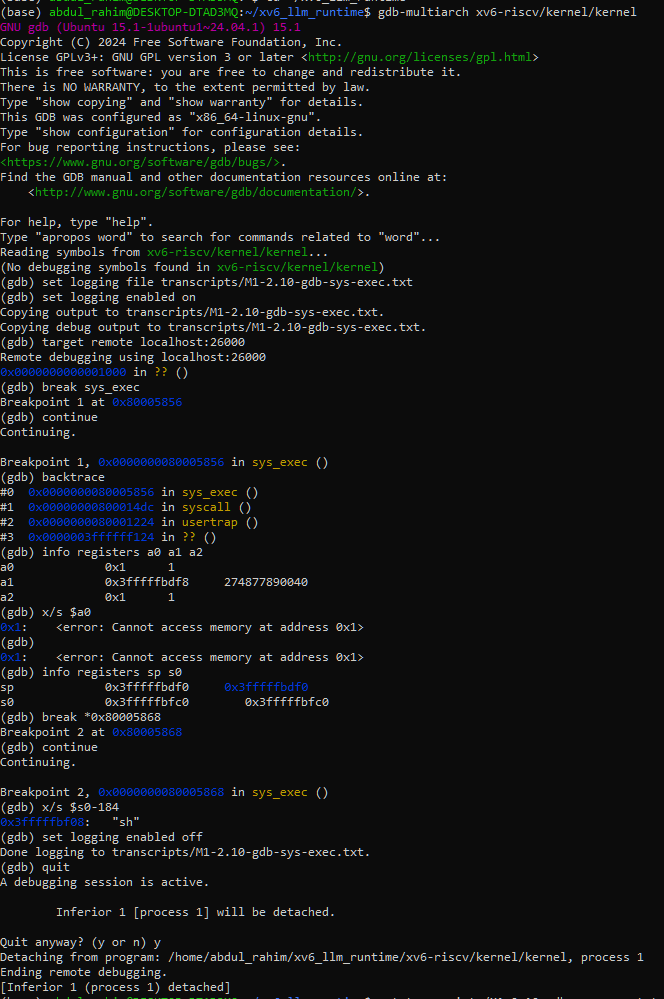
\includegraphics[width=0.88\textwidth]{M1-2.10-01-gdb-sys-exec.png}
\caption{The kernel entry-point trace as captured. This session was reproduced identically twice, at the same addresses and with the same register values.}
\label{fig:gdb}
\end{figure}

\textbf{Trace Explanation:} The kernel was started under QEMU with GDB enabled, and GDB was attached to the running kernel through the remote debugging port. A breakpoint was placed on \texttt{sys\_exec}, causing execution to stop when the kernel reached that function. The \texttt{backtrace} command showed the active call chain as \texttt{sys\_exec} $\rightarrow$ \texttt{syscall} $\rightarrow$ \texttt{usertrap}, demonstrating how execution reached the selected kernel function from the trap-handling path; frame \#3 lies above \texttt{0x3ffffff000} and is unnamed because it is user-space, outside the kernel's symbol table.

Two details deserve comment. First, GDB placed the breakpoint at \texttt{0x80005856} rather than at \texttt{sys\_exec}'s entry (\texttt{0x80005838}) because it skips the function prologue. At that point the argument registers hold the arguments being marshalled for the \emph{next} call, \texttt{argaddr(1, ...)}, not \texttt{sys\_exec}'s own --- which is why \texttt{a0} reads \texttt{0x1}, an argument index rather than a pointer.

Second, and this is the underlying reason, a system call's arguments never arrive in registers in xv6: the trap saves user state into the trapframe, and \texttt{sys\_exec} retrieves its arguments through \texttt{argaddr} and \texttt{argstr}, which read from there. Breaking after \texttt{argstr} returns and reading \texttt{s0-184} --- the buffer it was given --- yields \texttt{"sh"}, the program \texttt{init} was executing. The offset matches the disassembly exactly: \texttt{argstr(0, s0-184, 128)} at \texttt{0x8000585e}--\texttt{0x80005864}, and $\texttt{0x3fffffbfc0} - 184 = \texttt{0x3fffffbf08}$.

% =====================================================================
% =====================================================================
\section*{Section 3.1 --- Bring the System Up}
\addcontentsline{toc}{section}{Section 3.1 --- Bring the System Up}
% =====================================================================

All three configurations were brought up on the platform described above and a console transcript captured for each: the single node (\S3.1.1), the multi-node ring (\S3.1.2), and the weight-fetch path (\S3.1.3). Each transcript below is unedited console output, with the screenshot of the same run beside it. The commands are repeated in runbook order in Section 3.2, Phase 2, so that section can be followed on its own.

A first sanity boot confirms the kernel and filesystem image are intact:

\begin{lstlisting}[language=bash]
./boot.sh
# at the xv6 $ prompt:
ls
\end{lstlisting}

\begin{figure}[H]
\centering
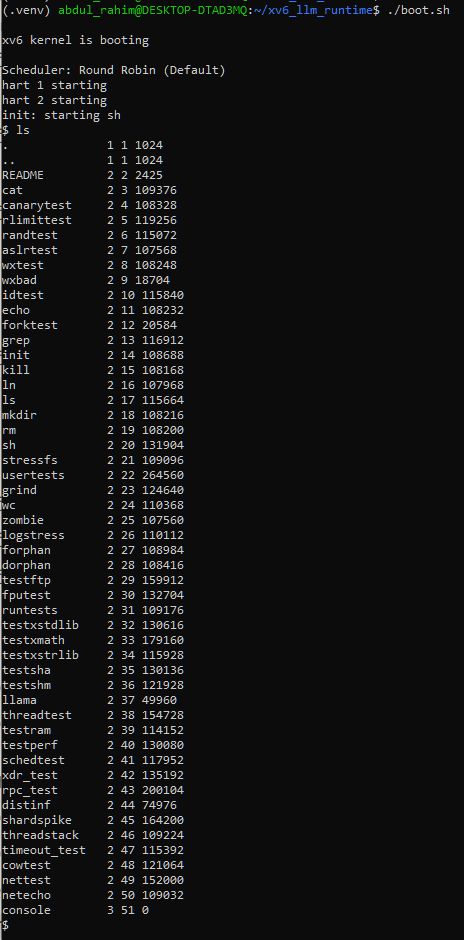
\includegraphics[height=0.48\textheight]{M1-2.5-01-xv6-boot-and-ls.png}
\caption{First boot and filesystem listing. \texttt{llama}, \texttt{testftp}, \texttt{distinf} and \texttt{usertests} are all present in \texttt{fs.img}.}
\label{fig:boot-ls}
\end{figure}

\subsection*{3.1.1 Single Node}

Requires two separate terminal windows.

\textbf{Terminal 1 (Weight Server):}
\begin{lstlisting}[language=bash]
python server/server.py
\end{lstlisting}

Expected: three \texttt{Loaded file} lines (ids 1, 2, 3, with sizes and SHA-256 prefixes) followed by \texttt{Server listening on 0.0.0.0:9999 (UDP)}, and no \texttt{ERROR} lines. Leave it running.

\begin{figure}[H]
\centering
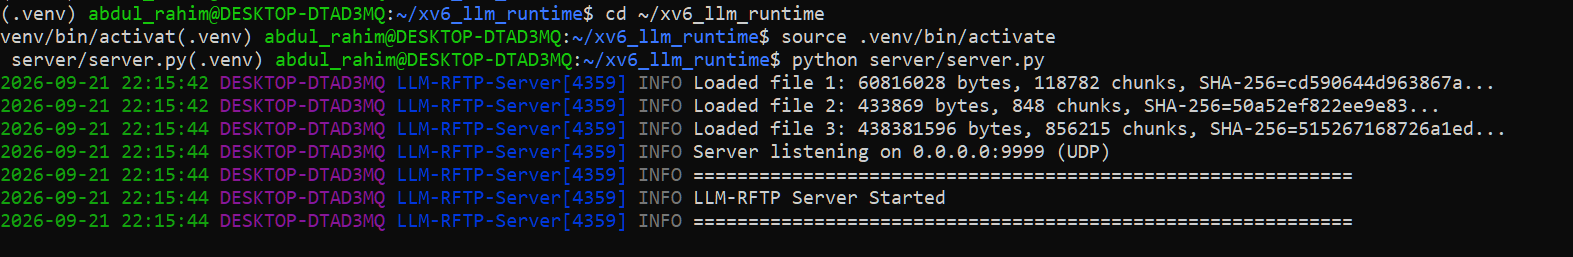
\includegraphics[width=0.94\textwidth]{M1-2.6-01-weight-server-loaded.png}
\caption{Weight server ready. All three checkpoints are loaded into memory and their digests match Figure~\ref{fig:checkpoints}.}
\label{fig:weight-server}
\end{figure}

\textbf{Terminal 2 (xv6 OS Runtime):}
\begin{lstlisting}[language=bash]
./boot.sh
\end{lstlisting}

Once the xv6 \texttt{\$} prompt appears, run:
\begin{lstlisting}[language=bash]
llama -n 32 -i "Once upon a time" -t 0
\end{lstlisting}

\texttt{-t 0} fixes temperature at zero so the output is deterministic and runs are comparable; this is required for every measured run. The first invocation after boot prints \texttt{Fetching from server...} and pauses for 60 to 90 seconds while the 60~MB checkpoint crosses the emulated UDP link in 512-byte chunks. This is expected, not a hang. Subsequent \texttt{llama} runs in the same boot start immediately from the shared-memory cache.

\textbf{Validated Output Transcript:}
\begin{lstlisting}[basicstyle=\ttfamily\scriptsize]
$ llama -t 0 -n 32 -i "Once upon a time"
 No cached data found for llm_weights. Fetching from server...
PASS    llm_weights fetched and cached in shared memory (ID: 0).

 No cached data found for llm_tokenizer. Fetching from server...
PASS    llm_tokenizer fetched and cached in shared memory (ID: 1).

thread_create: sharing user memory with main process (pid=3)
thread_create: sharing user memory with main process (pid=3)
thread_create: sharing user memory with main process (pid=3)
Once upon a time, there was a little girl named Lily. She loved to play
outside in the sunshine. One day, she saw a big

achieved tok/s: 5.974176

==================================================================
                       FUNCTION PROFILING
==================================================================
            Function    Calls Total(ms) Self(ms)  Avg(ms)  Time(%)
------------------------------------------------------------------
 fetch_model_weights        1    56610    56610 56610.00   89.83%
              matmul     1376     4559     4640     3.31    7.36%
     fetch_tokenizer        1      616      616   616.00    0.97%
             forward       32     5265      461   164.53    0.73%
              encode        1      336      336   336.00    0.53%
            generate        1     5730      103  5730.00    0.16%
 multihead_attention      192       78       94     0.40    0.14%
             rmsnorm      416       35       71     0.08    0.11%
   build_transformer        1       33       33    33.00    0.05%
     build_tokenizer        1       22       23    22.00    0.03%
              sample       28       13       15     0.46    0.02%
              decode       32        5       10     0.15    0.01%
       build_sampler        1        1        1     1.00    0.00%
==================================================================
Total Time: 63123 ms

==================================================================
                     SYSTEM PERFORMANCE METRICS
==================================================================

MEMORY USAGE:
          Initial      1.7 MB (1843200 bytes)
             Peak     66.5 MB (69750784 bytes)
            Final     66.5 MB (69750784 bytes)

TIMING:
     Total (E2EL)    63123 ms
        Inference     5189 ms

LLM METRICS:
             TTFT    58696 ms

THROUGHPUT:
        Generated       31 tokens
             Rate     5.97 tokens/sec
==================================================================
$
\end{lstlisting}

\begin{figure}[H]
\centering
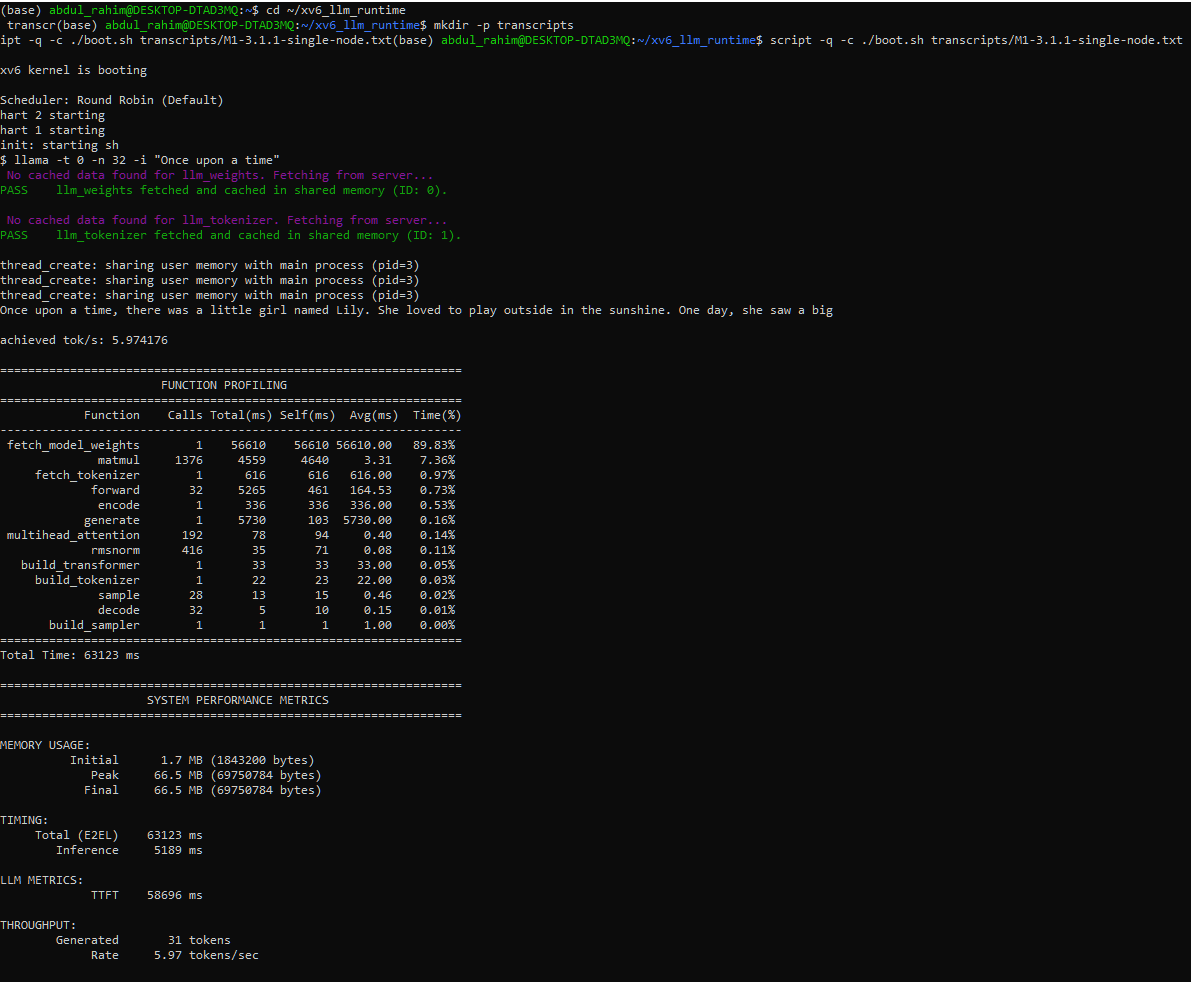
\includegraphics[height=0.56\textheight]{M1-2.6-02-single-node-generation.png}
\caption{Single-node generation as captured. Note that \texttt{fetch\_model\_weights} alone accounts for 89.8\% of elapsed time --- transferring the checkpoint costs an order of magnitude more than using it.}
\label{fig:single-node}
\end{figure}

\subsection*{3.1.2 Multi-Node Ring}

Automatically provisions a master node and two workers via QEMU multicast without requiring root privileges. Stop \texttt{server.py} first (\texttt{Ctrl-C}): the simulator starts its own weight server.

\begin{lstlisting}[language=bash, showstringspaces=false]
pkill -f qemu-system-riscv64; pkill -f mcast_switch.py
python server/distinf_sim.py --workers 2 --model 1 --steps 32 --prompt "Once upon a time"
\end{lstlisting}

The \texttt{pkill} is mandatory before every ring run. All nodes share one multicast segment with compile-time MAC addresses, so a leftover QEMU from a previous run produces a duplicate-address collision whose symptom --- a weight fetch that never completes --- is indistinguishable from a code fault.

\textbf{Validated Output Transcript:}
\begin{lstlisting}[basicstyle=\ttfamily\scriptsize]
[sim] staging 3 prebuilt node image(s)...
[sim] starting host mcast switch (weight server on the segment)...
[sim] booting 3 node(s) (timeout 240s each)...
[sim] master: expecting 2 worker(s), model 1 (stories15M), 32 tokens
[sim] OK  worker1 registered (0.7s)
[sim] OK  worker2 registered (0.7s)
[sim] OK  2 worker(s) registered (serialized)
[sim] OK  layers assigned
[sim] OK  worker1 shard resident (32s)
[sim] OK  worker2 shard resident (33s)
[sim] OK  all shards resident -- generating

[sim] ==== generated ====
Once upon a time , there was a little girl named L ily . She loved to play
outside in the sun sh ine . One day , she saw a big
[sim] ===================
[sim] ==================== run summary ====================
[sim]  topology      master 10.0.0.2 + 2 worker(s) | model 1 (stories15M) | 32 steps
[sim]  build         3 image(s) in 0s
[sim]  boot          master 6s | worker1 6s | worker2 6s
[sim]  registration  worker1 0.7s | worker2 0.7s   (serialized)
[sim]  layers        w1 [0,3) | w2 [3,6)
[sim]  shard fetch   worker1 32s | worker2 33s
[sim]  final ring    2/2 worker(s)
[sim]  generation    32 token(s) in 50.1s
[sim]  latency       latency/token (avg over 32): ring rtt 1453882 us =
                     compute 261205 us + network 1192677 us | master 177060 us
                     | 0.6 tok/s
[sim]  rpc drops     malformed 0 | rate-limited 0 | bad-prog 0 | unknown-proc 0
[sim]  logs          /tmp/distinf_sim/{master,worker1..N}.log
[sim]  result        PASS
[sim] =====================================================
[sim] PASS
\end{lstlisting}

\begin{figure}[H]
\centering
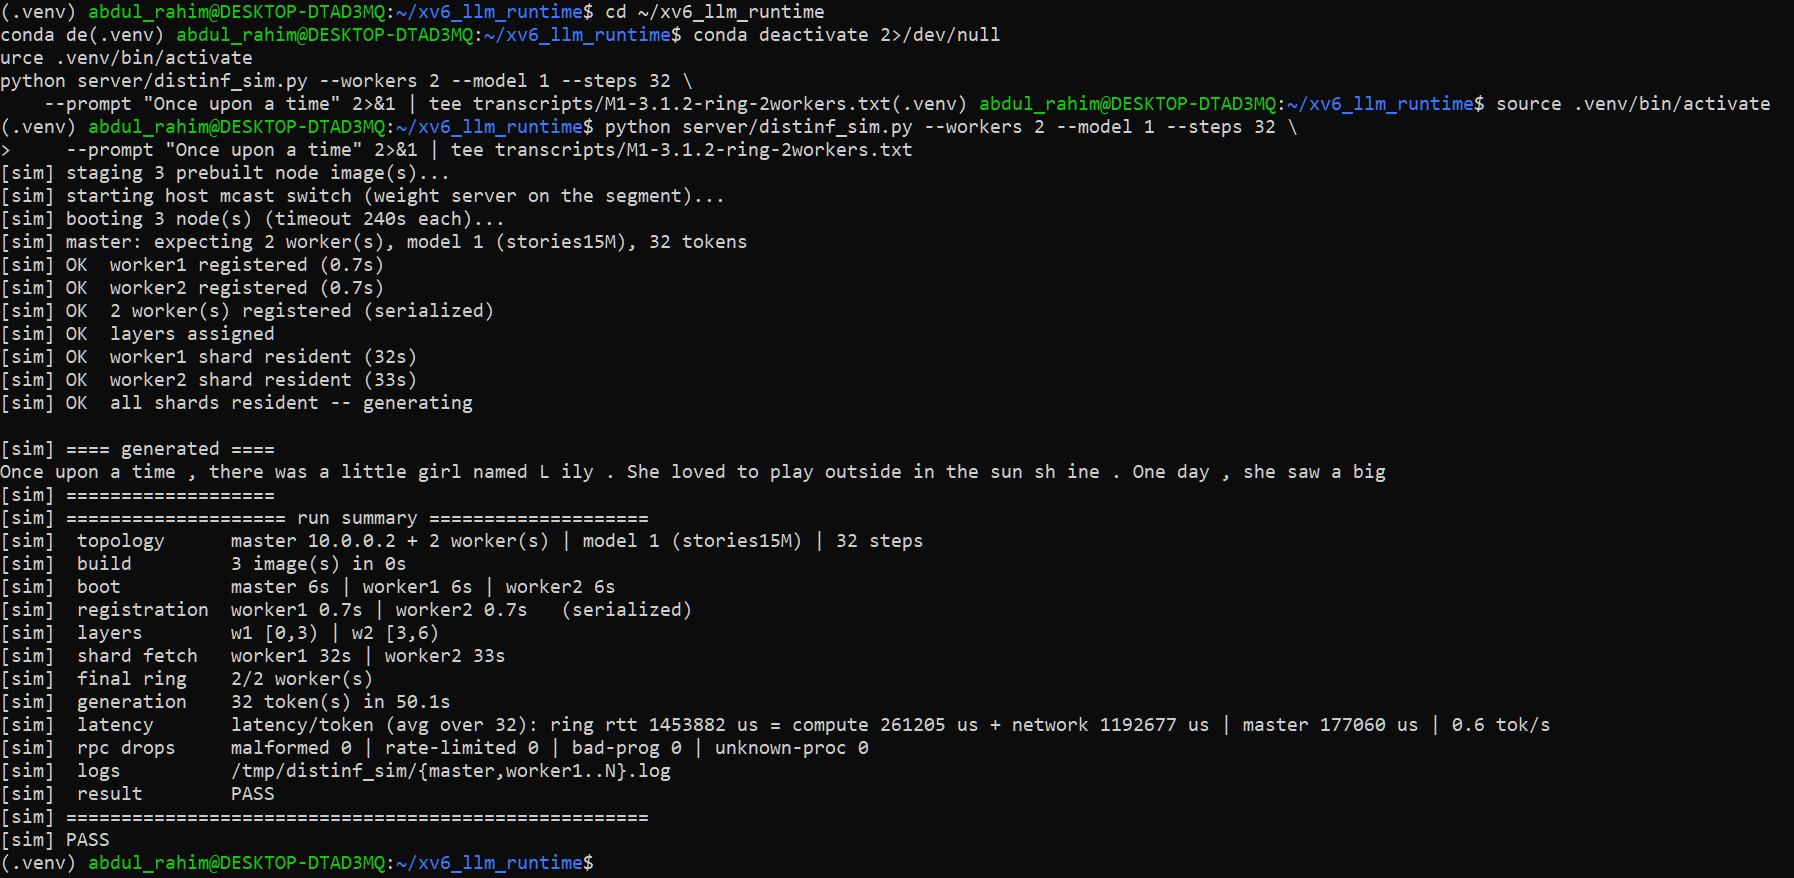
\includegraphics[width=0.98\textwidth]{M1-2.7-01-ring-2workers.png}
\caption{Two-worker ring. Both workers register, layers are assigned \texttt{w1 [0,3)} and \texttt{w2 [3,6)}, both shards become resident, and the run ends \texttt{result PASS}.}
\label{fig:ring-2w}
\end{figure}

The ring reproduces the single-node token stream exactly. The only visible difference is that the simulator prints per-token rather than per-character, making token boundaries visible (``L ily'', ``sun sh ine''). That the two agree is the strongest single piece of evidence that sharding the model preserves the computation.

\subsection*{3.1.3 Weight-Fetch Path}

Validates that the network transport can deliver byte-exact ranges of the model checkpoint. The automated suite is run through \texttt{pytest}:

\begin{lstlisting}[language=bash]
pytest server/weightfetch_regression_test.py -v --noconftest
\end{lstlisting}

\textbf{Note:} this suite must be invoked through \texttt{pytest}. Running \texttt{python server/\allowbreak{}weightfetch\_\allowbreak{}regression\_\allowbreak{}test.py} executes the file as a plain script, runs no tests at all, and exits 0 --- which is easily mistaken for a pass.

To verify network transport integrity and segment retrieval for the runtime, the \texttt{testftp} utility was also executed directly within the xv6 terminal shell against the host weight server:

\begin{lstlisting}[basicstyle=\ttfamily\scriptsize]
$ testftp
Starting LLM file transfer test...
PASS    Successfully fetched tokenizer: 433869 bytes
  Final SHA-256: 50a52ef822ee9e83de5ce9d0be0a025a773d019437f58b5ff9dcafb063ece361
---
 PASS    Successfully fetched weights: 60816028 bytes
  Final SHA-256: cd590644d963867a2b6e5a1107f51fad663c41d79c149fbecbbb1f95fa81f49a
PASS   LLM file transfer test completed
$
\end{lstlisting}

\begin{figure}[H]
\centering
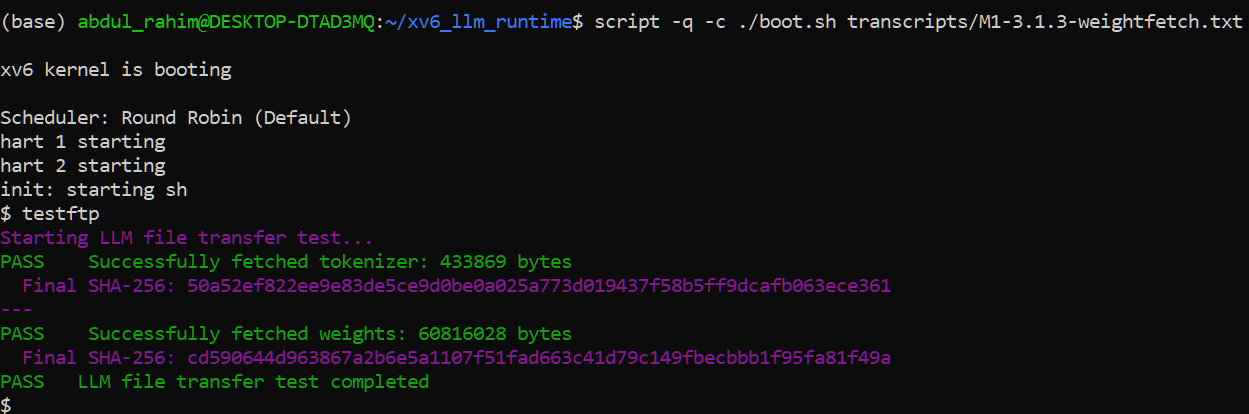
\includegraphics[width=0.94\textwidth]{M1-3.1.3-01-testftp-bytes.png}
\caption{\texttt{testftp} run from the xv6 shell. Both byte counts and both digests match Figure~\ref{fig:checkpoints} exactly, so the transfer is byte-exact end to end.}
\label{fig:testftp}
\end{figure}

\section*{Section 3.2 --- Runbook}
\addcontentsline{toc}{section}{Section 3.2 --- Runbook}
% =====================================================================

This runbook was validated end-to-end on a clean WSL (Ubuntu 24.04) terminal environment and reproduces all three execution configurations described in Sections 3.1.1--3.1.3 of the assignment. It was subsequently re-executed from scratch as a second validation pass, which surfaced one path error in Phase 3; that error is corrected below and noted in place.

\subsection*{Phase 1: Prerequisites and Environment Setup}

\textbf{Step 1 --- Clone the repository:}
\begin{lstlisting}[language=bash]
cd ~
git clone https://github.com/aliyafatima001100-pixel/xv6_llm_runtime.git
cd xv6_llm_runtime
\end{lstlisting}

All subsequent commands are run from this directory.

\textbf{Step 2 --- Install system dependencies:}
\begin{lstlisting}[language=bash]
sudo apt update
sudo apt install -y git build-essential gdb-multiarch qemu-system-misc \
    gcc-riscv64-linux-gnu binutils-riscv64-unknown-elf \
    python3-venv python3-pip unzip
\end{lstlisting}

Two notes, both of which cost us time during bring-up:

\begin{itemize}[leftmargin=1.4cm]
\item The package providing \texttt{qemu-system-riscv64} is \texttt{qemu-system-misc}. There is no package named \texttt{qemu-system-riscv}; asking for it aborts the install with \texttt{Unable to locate package}.
\item \texttt{python3-venv} is required. A stock Ubuntu image fails Step 3 with \texttt{ensurepip is not available} without it.
\end{itemize}

\textbf{Step 2a --- Verify the toolchain} before continuing. All three commands must print a version string:
\begin{lstlisting}[language=bash]
qemu-system-riscv64 --version
riscv64-unknown-elf-objdump --version | head -1
gdb-multiarch --version | head -1
\end{lstlisting}

\begin{figure}[H]
\centering
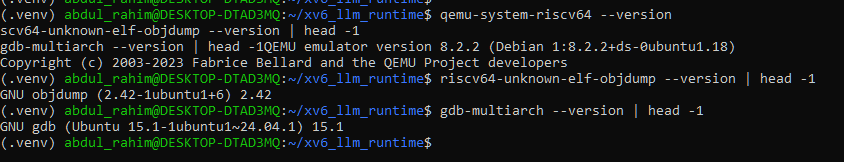
\includegraphics[width=0.86\textwidth]{M1-2.2-01-toolchain-versions.png}
\caption{Toolchain verification: QEMU 8.2.2, objdump 2.42, GDB 15.1. If any of these reports \texttt{command not found}, nothing further in this runbook will work.}
\label{fig:toolchain}
\end{figure}

\textbf{Step 3 --- Set up the Python virtual environment and networking tools:}
\begin{lstlisting}[language=bash]
python3 -m venv .venv
source .venv/bin/activate
pip install scapy pytest coloredlogs
\end{lstlisting}

The virtual environment must be created \emph{inside} the repository, because the project's own scripts refer to \texttt{.venv/bin/python} by that relative path. \texttt{source .venv/bin/activate} must be repeated in every new terminal; Phase 2 uses two terminals concurrently. If Anaconda is installed and auto-activates, run \texttt{conda deactivate} first, otherwise the base environment competes with the project's own.

\textbf{Step 4 --- Fetch the AI model weights:}
\begin{lstlisting}[language=bash]
chmod +x boot.sh boot-gdb.sh fetch-models.sh
./fetch-models.sh
./fetch-models.sh --check
\end{lstlisting}

This downloads roughly 495~MB (about 2.5 minutes at 4.5~MB/s) and verifies size and SHA-256 for each file. Expected output of \texttt{--check}:

\begin{lstlisting}
OK      tokenizer.bin (433869 bytes)
OK      stories15M.bin (60816028 bytes)
OK      stories110M.bin (438381596 bytes)
all three checkpoints present and verified in server/models
\end{lstlisting}

\begin{figure}[H]
\centering
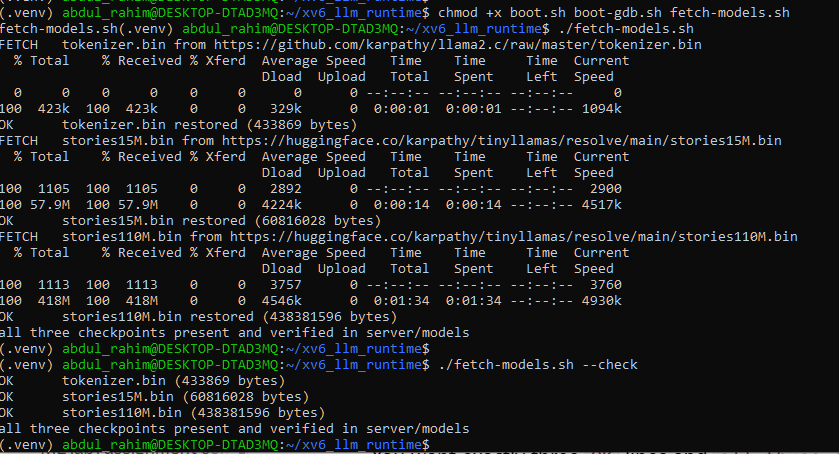
\includegraphics[width=0.86\textwidth]{M1-2.4-01-checkpoints-verified.png}
\caption{Checkpoint fetch and verification. These digests are the reference against which the weight-fetch transcript in Part C is checked.}
\label{fig:checkpoints}
\end{figure}

\subsection*{Phase 2: Execution Configurations}

The Python virtual environment must be active (\texttt{source .venv/bin/activate}) before running any configuration below. Exit QEMU at any point with \texttt{Ctrl-A}, release, then \texttt{x}; closing the terminal instead leaves QEMU running and causes address collisions in later runs.

These are the commands in the order a reader should run them. The transcript each produces, and a screenshot of it, are in Section 3.1.

\textbf{Sanity boot} --- confirms the kernel and filesystem image are intact (Figure~\ref{fig:boot-ls}):

\begin{lstlisting}[language=bash]
./boot.sh
# at the xv6 $ prompt:
ls
\end{lstlisting}

\textbf{Single node} (\S3.1.1; Figures~\ref{fig:weight-server} and~\ref{fig:single-node}) --- two terminals:

\begin{lstlisting}[language=bash]
# terminal 1
python server/server.py

# terminal 2
./boot.sh
# at the xv6 $ prompt:
llama -n 32 -i "Once upon a time" -t 0
\end{lstlisting}

\texttt{-t 0} is mandatory for every measured run. The default temperature of 1.0 samples randomly and no two runs match; only \texttt{-t 0} takes the greedy path.

\textbf{Multi-node ring} (\S3.1.2; Figure~\ref{fig:ring-2w}) --- stop \texttt{server.py} first, the simulator starts its own:

\begin{lstlisting}[language=bash, showstringspaces=false]
pkill -f qemu-system-riscv64; pkill -f mcast_switch.py
python server/distinf_sim.py --workers 2 --model 1 --steps 32 --prompt "Once upon a time"
\end{lstlisting}

The \texttt{pkill} is mandatory before every ring run. All nodes share one multicast segment with compile-time MAC addresses, so a leftover QEMU from a previous run produces a duplicate-address collision whose symptom --- a weight fetch that never completes --- is indistinguishable from a code fault.

\textbf{Weight-fetch path} (\S3.1.3; Figure~\ref{fig:testftp}) --- two terminals again:

\begin{lstlisting}[language=bash]
# terminal 1
python server/server.py

# terminal 2
./boot.sh
# at the xv6 $ prompt:
testftp
\end{lstlisting}


\subsection*{Phase 3: Regression Suites}

Run from the repository root with \texttt{.venv} active, after \texttt{pkill -f qemu-system-riscv64}:

\begin{lstlisting}[language=bash]
pytest server/kernel_regression_test.py      -v --noconftest
pytest server/weightfetch_regression_test.py -v --noconftest
pytest server/distinf_regression_test.py     -v --noconftest
\end{lstlisting}

\begin{table}[H]
\centering
\begin{tabular}{lll}
\toprule
\textbf{Suite} & \textbf{Expected} & \textbf{Observed runtime} \\
\midrule
\texttt{kernel\_regression\_test.py}      & 14 passed            & 128~s \\
\texttt{weightfetch\_regression\_test.py} & 4 passed, 0 skipped  & 27~s \\
\texttt{distinf\_regression\_test.py}     & 2 passed, 6 skipped  & 187~s \\
\bottomrule
\end{tabular}
\caption{Regression suite results on an unmodified checkout. All three match the handout's expected counts exactly, so there is no deviation to record in the observations log.}
\label{tab:suites}
\end{table}

\begin{figure}[H]
\centering
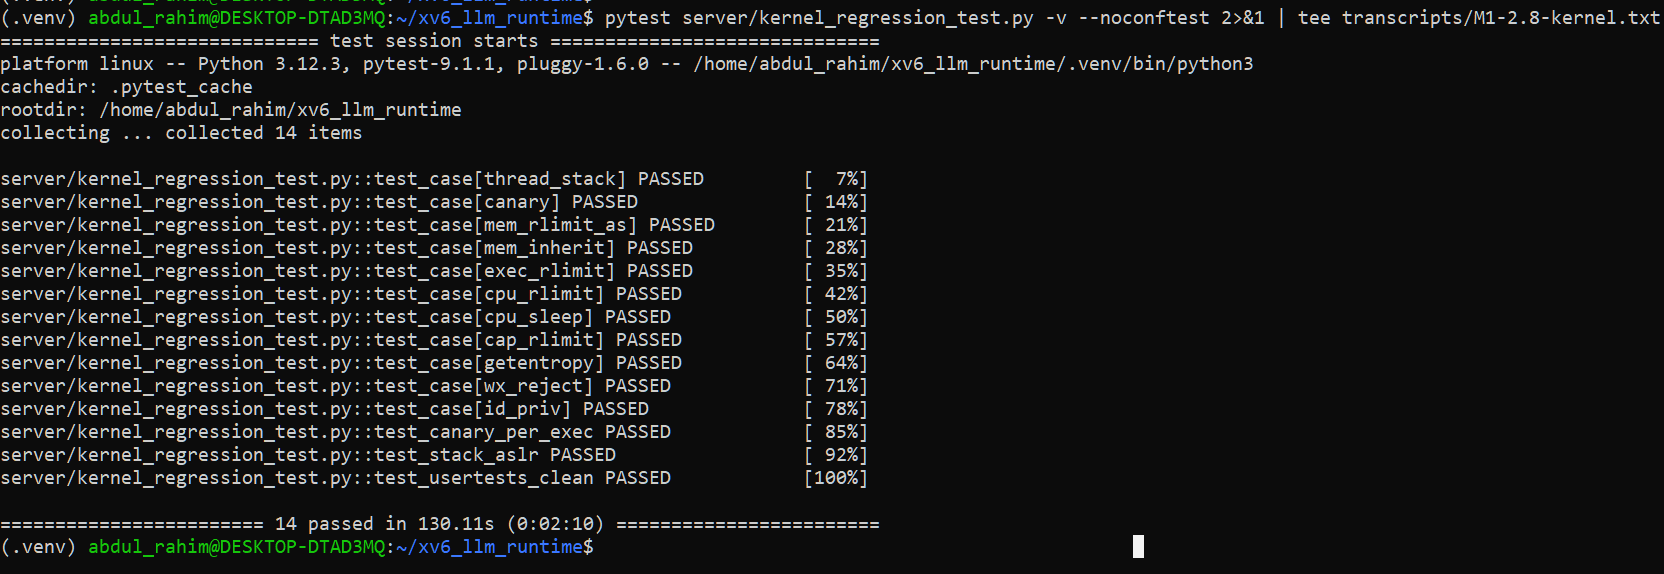
\includegraphics[width=0.96\textwidth]{M1-2.8-01-kernel-regression.png}
\caption{L1 kernel hardening suite: 14 passed, including a full \texttt{usertests} pass. The case names map directly onto the hardening set in Section~3.3, row 8 --- canary, \texttt{RLIMIT\_AS}, limit inheritance across \texttt{fork}, capability drop, \texttt{getentropy}, W\^{}X rejection and stack ASLR.}
\label{fig:kernel-regression}
\end{figure}

\begin{figure}[H]
\centering
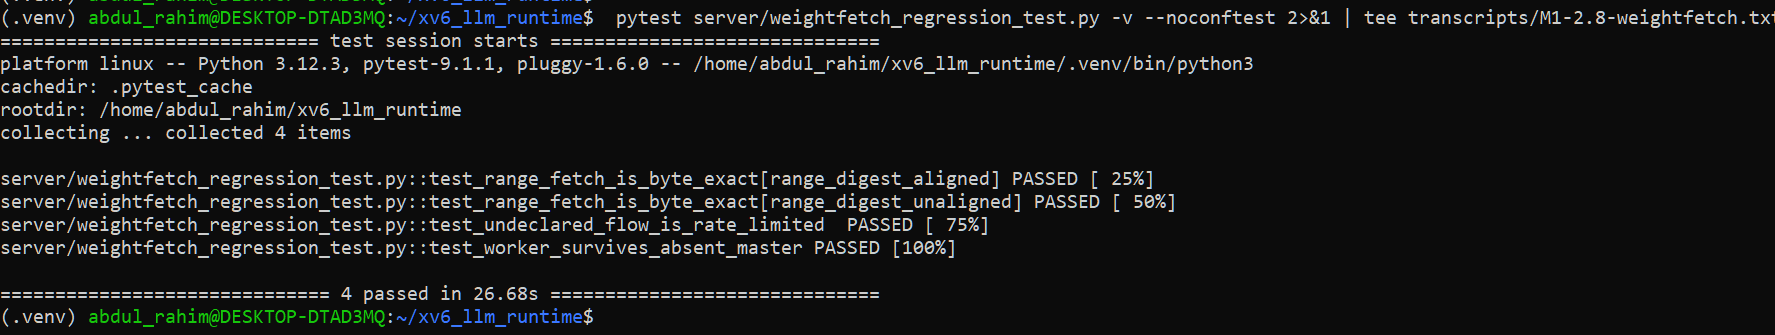
\includegraphics[width=0.96\textwidth]{M1-2.8-02-weightfetch-regression.png}
\caption{Weight-fetch suite: 4 passed, 0 skipped. A skip here would indicate a missing 110M checkpoint rather than a failure.}
\label{fig:weightfetch-regression}
\end{figure}

\begin{figure}[H]
\centering
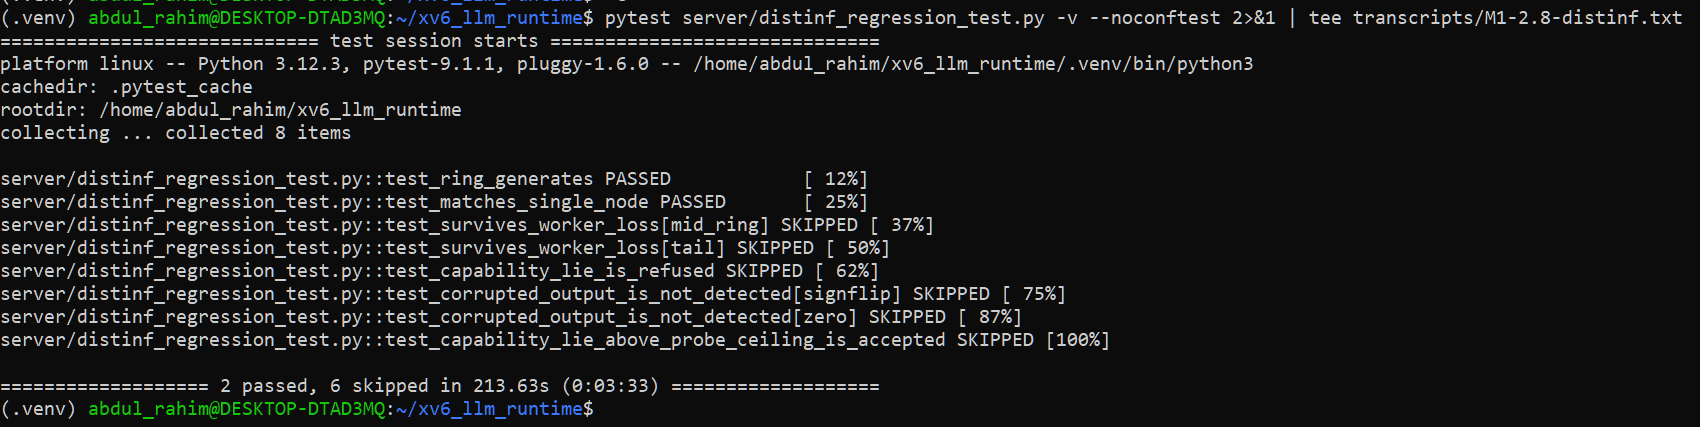
\includegraphics[width=0.96\textwidth]{M1-2.8-03-distinf-regression.png}
\caption{Distributed inference suite: 2 passed, 6 skipped, with explicit skip reasons (\texttt{long run; set DISTINF\_SCALE=1}). The test names themselves are worth reading: \texttt{test\_corrupted\_output\_is\_not\_detected} and \texttt{test\_capability\_lie\_above\_probe\_ceiling\_is\_accepted} assert that a defence is \emph{absent}, regression-locking a known gap so it cannot change unnoticed.}
\label{fig:distinf-regression}
\end{figure}

\texttt{net\_regression\_test.py} and \texttt{rpc\_regression\_test.py} are excluded: the first requires root and a tap device, the second requires a node already booted.

\subsection*{Phase 4: Studying the Kernel Binary}

\begin{lstlisting}[language=bash]
cd ~/xv6_llm_runtime/xv6-riscv
riscv64-unknown-elf-nm kernel/kernel | grep -E ' [tT] ' | sort > kernel-symbols.txt
riscv64-unknown-elf-objdump -d kernel/kernel > kernel-disassembly.txt
riscv64-unknown-elf-objdump -d --disassemble=sys_exec kernel/kernel
cd ~/xv6_llm_runtime
\end{lstlisting}

The full disassembly runs to 15{,}794 lines and is worth keeping on disk rather than regenerating: the architecture map in Section 3.3 is built by grepping it.

\begin{figure}[H]
\centering
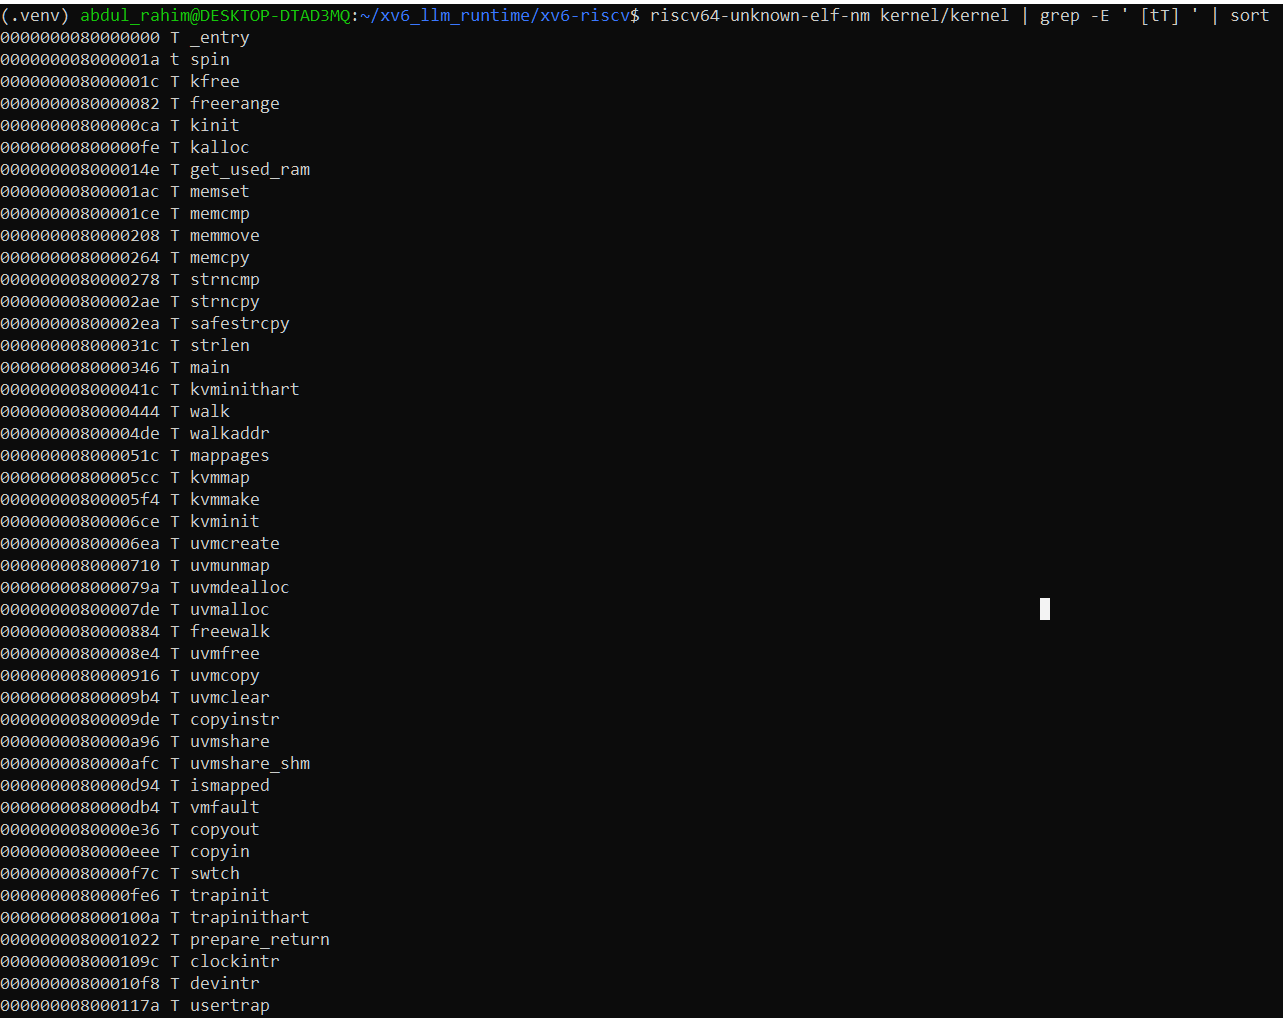
\includegraphics[width=0.58\textwidth]{M1-2.9-01-kernel-symbols.png}
\caption{Part of the kernel symbol table. This is the only map into the kernel, whose \texttt{.c} sources were deliberately withheld.}
\label{fig:kernel-symbols}
\end{figure}

\begin{figure}[H]
\centering
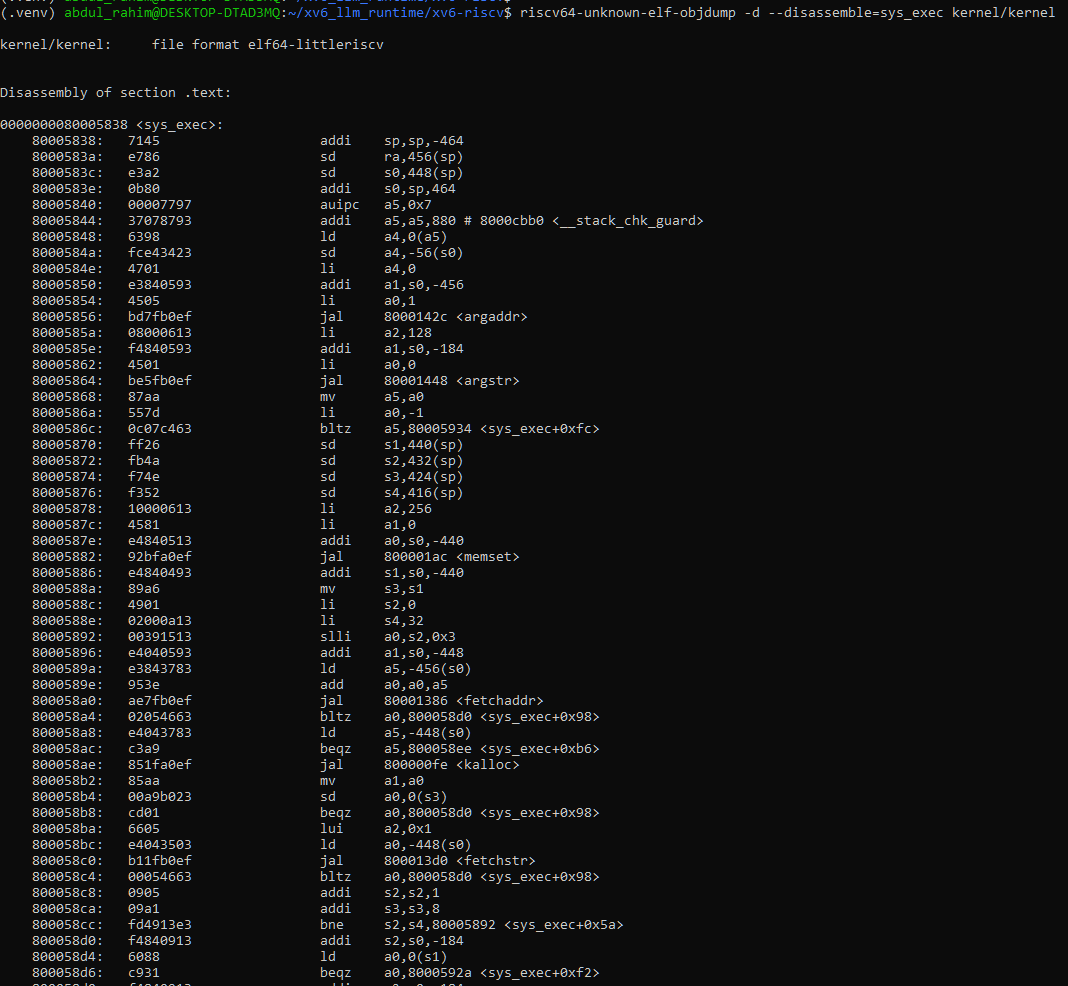
\includegraphics[width=0.80\textwidth]{M1-2.9-02-disas-sys-exec.png}
\caption{Disassembly of \texttt{sys\_exec}. The canary load from \texttt{\_\_stack\_chk\_guard} at \texttt{0x8000cbb0} and its store to \texttt{s0-56} are visible at the top; the XOR check and branch to \texttt{\_\_stack\_chk\_fail} at the bottom. This single listing supplies the stack-placement detail F6 requires.}
\label{fig:disas-sysexec}
\end{figure}

Under the debugger, two terminals, \textbf{both starting from the repository root}:

\begin{lstlisting}[language=bash]
# Terminal 1
./boot-gdb.sh          # prints nothing and returns no prompt: this is correct

# Terminal 2
gdb-multiarch xv6-riscv/kernel/kernel
(gdb) target remote localhost:26000
(gdb) break sys_exec
(gdb) continue
(gdb) backtrace
\end{lstlisting}

\texttt{(No debugging symbols found)} is expected: the kernel ships with its symbol table but without DWARF debug information.

\paragraph{Correction found during the validation pass.}
\texttt{gdb-multiarch} must be launched from the repository root. An earlier draft of this phase left the reader inside \texttt{xv6-riscv/} after the \texttt{objdump} commands and then gave the path \texttt{xv6-riscv/kernel/kernel}, which from there resolves to \texttt{xv6-riscv/\allowbreak{}xv6-riscv/\allowbreak{}kernel/\allowbreak{}kernel}. The failure is quiet and misleading: GDB starts with no binary loaded, and every subsequent command reports \texttt{No symbol table is loaded} rather than naming the real cause. The \texttt{cd} back to the repository root above is the fix.

% =====================================================================
\section*{Section 3.3 --- Architecture Map}
\addcontentsline{toc}{section}{Section 3.3 --- Architecture Map}
% =====================================================================

The table below maps the system's eight major subsystems: responsibility, entry point, source location (or symbol-table address for the two kernel-only rows), and the standards each implements. Every source line and symbol address below was verified against the shipped headers and the symbol table generated in Section 3.2, Phase 4.

\begingroup\scriptsize
\begin{longtable}{@{}R{0.145}R{0.315}R{0.251}R{0.289}@{}}
\toprule
\textbf{Subsystem} & \textbf{Responsibility} & \textbf{Entry Point / Location} & \textbf{Implemented Standards} \\
\midrule
\endhead

1. Network Stack &
Receives incoming network frames, validates minimum length (42 bytes), parses the EtherType field (bytes 12--13), and routes the packet to the ARP or IPv4 handlers or drops it via \texttt{kfree}. &
\texttt{net\_rx} \newline Addr.\ \texttt{0x800099c6} (from \texttt{nm} symbol table) &
RFC 791 (total length, fragment reassembly keyed on src/dst/proto/id); RFC 792 \& RFC 1122 \S3.2.2 (ICMP types, silent discard of unknown); RFC 1812 \S4.3.2.8 (ICMP generation rate limit); RFC 1918/3927/5737/5771/6598 (bogon filter) --- all cited in \texttt{kernel/net.h} \\
\midrule

2. Remote Procedure Call &
Implements the ONC RPC message layer: message timeouts (Section 5), authentication limits (Section 8.2), and remote calls over UDP. &
\texttt{rpc\_call} \newline \texttt{user/rpc.c:487} &
RFC 5531 (ONC RPC wire structures, field order, \S5 caller-side retransmission, \S8.2 auth body limit of 400~B, \S10.1 AUTH\_NONE mandatory, \S12); RFC 4506 (XDR encoding) \\
\midrule

3. Data Serialisation &
Initialises an XDR (External Data Representation) stream in memory to encode/decode data structures into an architecture-independent wire format. &
\texttt{xdrmem\_create} \newline \texttt{user/xdr.c:143} &
RFC 4506 (\texttt{xdr.c} itself carries no RFC comment; \texttt{rpc.h}, Row 2, and \texttt{distinf.h} explicitly state all XDR encoding follows RFC 4506) \\
\midrule

4. Discovery and Registration &
Manages cluster membership: worker registration, cryptographic identity verification, node heartbeats; maintains the ring's ``soft state'' and evicts unresponsive nodes. &
\texttt{discovery\_handle\_call} \newline \texttt{user/discovery.c:699} &
RFC 2104 / FIPS 198-1 (HMAC-SHA256 identity); RFC 2205 (soft-state registry); RFC 4303 (anti-replay model). \texttt{discovery.h} explicitly places RFC 5403 RPCSEC\_GSS out of scope \\
\midrule

5. Ring Driver \& Shard Logic &
Orchestrates distributed AI execution across a ring of nodes: master/worker roles, shard allocation, anti-replay session checking, UDP data integrity, worker soft-state via heartbeats during long model downloads. &
\texttt{main} (dispatches to \texttt{master\_run\_token} :1056 and \texttt{worker\_inference\_hook} :605) \newline \texttt{user/distinf.c:1551} &
RFC 4506 \S4 (XDR activation encoding, ``unsigned integers as 32-bit''); RFC 791 (datagram sizing); RFC 768 (UDP checksum integrity) \\
\midrule

6. Transformer Kernels &
Executes the core mathematical operations of the Llama model --- multi-head attention, matrix multiplication (\texttt{matmul}), RMSNorm, softmax --- for a forward pass predicting the next token. &
\texttt{forward} \newline \texttt{user/llama\_core.c:742} &
N/A --- standard neural-network arithmetic; \texttt{llama\_core.h} cites no external standard \\
\midrule

7. Weight Fetch Client &
Requests and downloads the AI model weights and tokenizer over the network: chunk completeness tracked with a per-chunk bitmap, missing-chunk retransmission, final file-integrity verification against the server's SHA-256. &
\texttt{fetch\_model\_weights} \newline \texttt{user/ftpclient.c:716} &
RFC 768 (UDP checksums for integrity). LLM-RFTP itself is project-defined and specified in \texttt{server/README.md}, not an external standard \\
\midrule

8. Kernel Hardening Set &
Establishes the security surface. \texttt{stackguard\_init} generates a 64-bit random canary (\texttt{rand64}) stored in \texttt{\_\_stack\_chk\_guard}; \texttt{random\_init} seeds the entropy pool from the hardware timer (\texttt{rdtime}) and stack-pointer addresses; \texttt{capable} and \texttt{rlimit\_as\_ok} enforce capability-based access control and resource limits; \texttt{kexec} enforces W\^{}X at exec time. &
\texttt{stackguard\_init} \texttt{0x80001e64}; \texttt{\_\_stack\_chk\_fail} \texttt{0x80001e80}; \texttt{random\_init} \texttt{0x80002000}; \texttt{rand64} \texttt{0x80001f3c}; \texttt{rlimit\_as\_ok} \texttt{0x8000693a}; \texttt{capable} \texttt{0x800069d6}; \texttt{kexec} \texttt{0x8000489e} (from \texttt{nm} symbol table) &
IEEE Std 1003.1-2017: per-process resource limits \texttt{RLIMIT\_AS}, \texttt{RLIMIT\_CPU} (\texttt{kernel/\allowbreak{}rlimit.h:5,30--31}); POSIX.1e capability model, \texttt{CAP\_SYS\_RESOURCE} / \texttt{CAP\_NET\_ADMIN} (\texttt{kernel/\allowbreak{}capability.h:5,25--26}); POSIX \texttt{getentropy} 256-byte request ceiling (\texttt{kernel/random.h:11--14}); OpenBSD W\^{}X model with \texttt{PT\_\allowbreak{}OPENBSD\_\allowbreak{}WXNEEDED} exemption (\texttt{user/wxtest.c}) \\
\bottomrule
\caption{Eight-subsystem architecture map.}
\label{tab:arch-map}
\end{longtable}
\endgroup

\subsection*{Row 8 read from the binary}

The canary mechanism is directly observable in the disassembly (Figure~\ref{fig:disas-sysexec}). \texttt{sys\_exec} loads \texttt{\_\_stack\_chk\_guard} from \texttt{0x8000cbb0} at entry (\texttt{0x80005840}--\texttt{0x80005848}) and stores it at \texttt{s0-56} (\texttt{0x8000584a}); every return path reloads it, XORs against the saved copy, and branches to \texttt{\_\_stack\_chk\_fail} at \texttt{0x80001e80} on mismatch (\texttt{0x80005934}--\texttt{0x80005946}). Under the debugger with \texttt{s0 = 0x3fffffbfc0}, the canary slot resolves to \texttt{0x3fffffbf88} --- the same fact obtained from two independent sources, static and live.

W\^{}X is \emph{not} enforced by \texttt{flags2perm} at \texttt{0x80004884}; that function only maps ELF \texttt{PF\_X}/\texttt{PF\_W} bits onto \texttt{PTE\_X}/\texttt{PTE\_W}. It is enforced inside \texttt{kexec} at \texttt{0x8000489e}, which refuses a writable-and-executable segment lacking the \texttt{PT\_\allowbreak{}OPENBSD\_\allowbreak{}WXNEEDED} tag, as \texttt{user/wxtest.c} documents and the \texttt{wx\_reject} regression case (Figure~\ref{fig:kernel-regression}) confirms.

\begin{figure}[H]
\centering
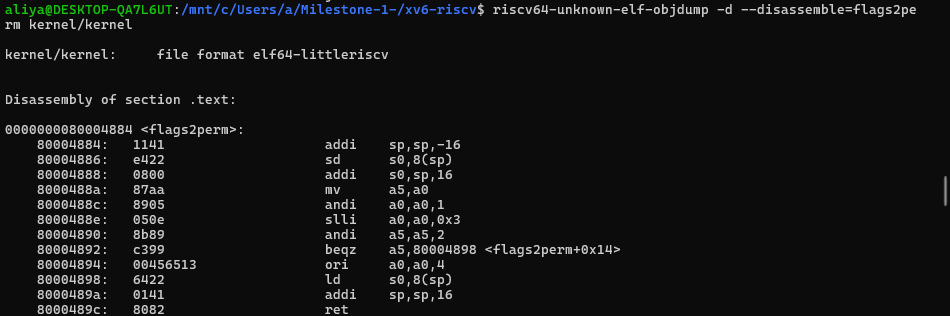
\includegraphics[width=0.80\textwidth]{row8_wx_flags2perm.png}
\caption{Disassembly of \texttt{flags2perm} at \texttt{0x80004884}. The function only sets \texttt{PTE\_X} from \texttt{PF\_X} (\texttt{andi a0,a0,1}; \texttt{slli a0,a0,0x3}) and conditionally ORs in \texttt{PTE\_W} from \texttt{PF\_W} (\texttt{andi a5,a5,2}; \texttt{ori a0,a0,4}); it contains no comparison, branch, or rejection logic of any kind. This confirms the W\^{}X check is not here --- it is entirely inside \texttt{kexec}.}
\label{fig:disas-flags2perm}
\end{figure}

% =====================================================================
\section*{Section 3.4 --- Figures}
\addcontentsline{toc}{section}{Section 3.4 --- Figures}
% =====================================================================

Figures F1--F7 below are drawn directly from the source referenced in Table~\ref{tab:arch-map}, the shipped headers, and the disassembly. Each figure's Mermaid source is given first, followed by the rendered image. The source shown is the source that produced the image.

\subsection*{F1 --- System Architecture}

\begin{lstlisting}[style=mermaid]
flowchart TD
    WS[("Weight server - server.py<br/>LLM-RFTP over UDP:9999")]
    M["Master 10.0.0.2<br/>embedding, sampler, classifier"]
    W1["Worker 1 10.0.0.3<br/>layers 0-1"]
    W2["Worker 2 10.0.0.4<br/>layers 2-3"]
    W3["Worker 3 10.0.0.5<br/>layers 4-5"]
    WS -. "tokenizer + head" .-> M
    WS -. "shard fetch<br/>512-byte chunks" .-> W1
    WS -. "shard fetch" .-> W2
    WS -. "shard fetch" .-> W3
    M ==>|"PROC_INFER_HOP"| W1
    W1 ==>|"activation"| W2
    W2 ==>|"activation"| W3
    W3 ==>|"final activation"| M
\end{lstlisting}

\begin{figure}[H]
\centering
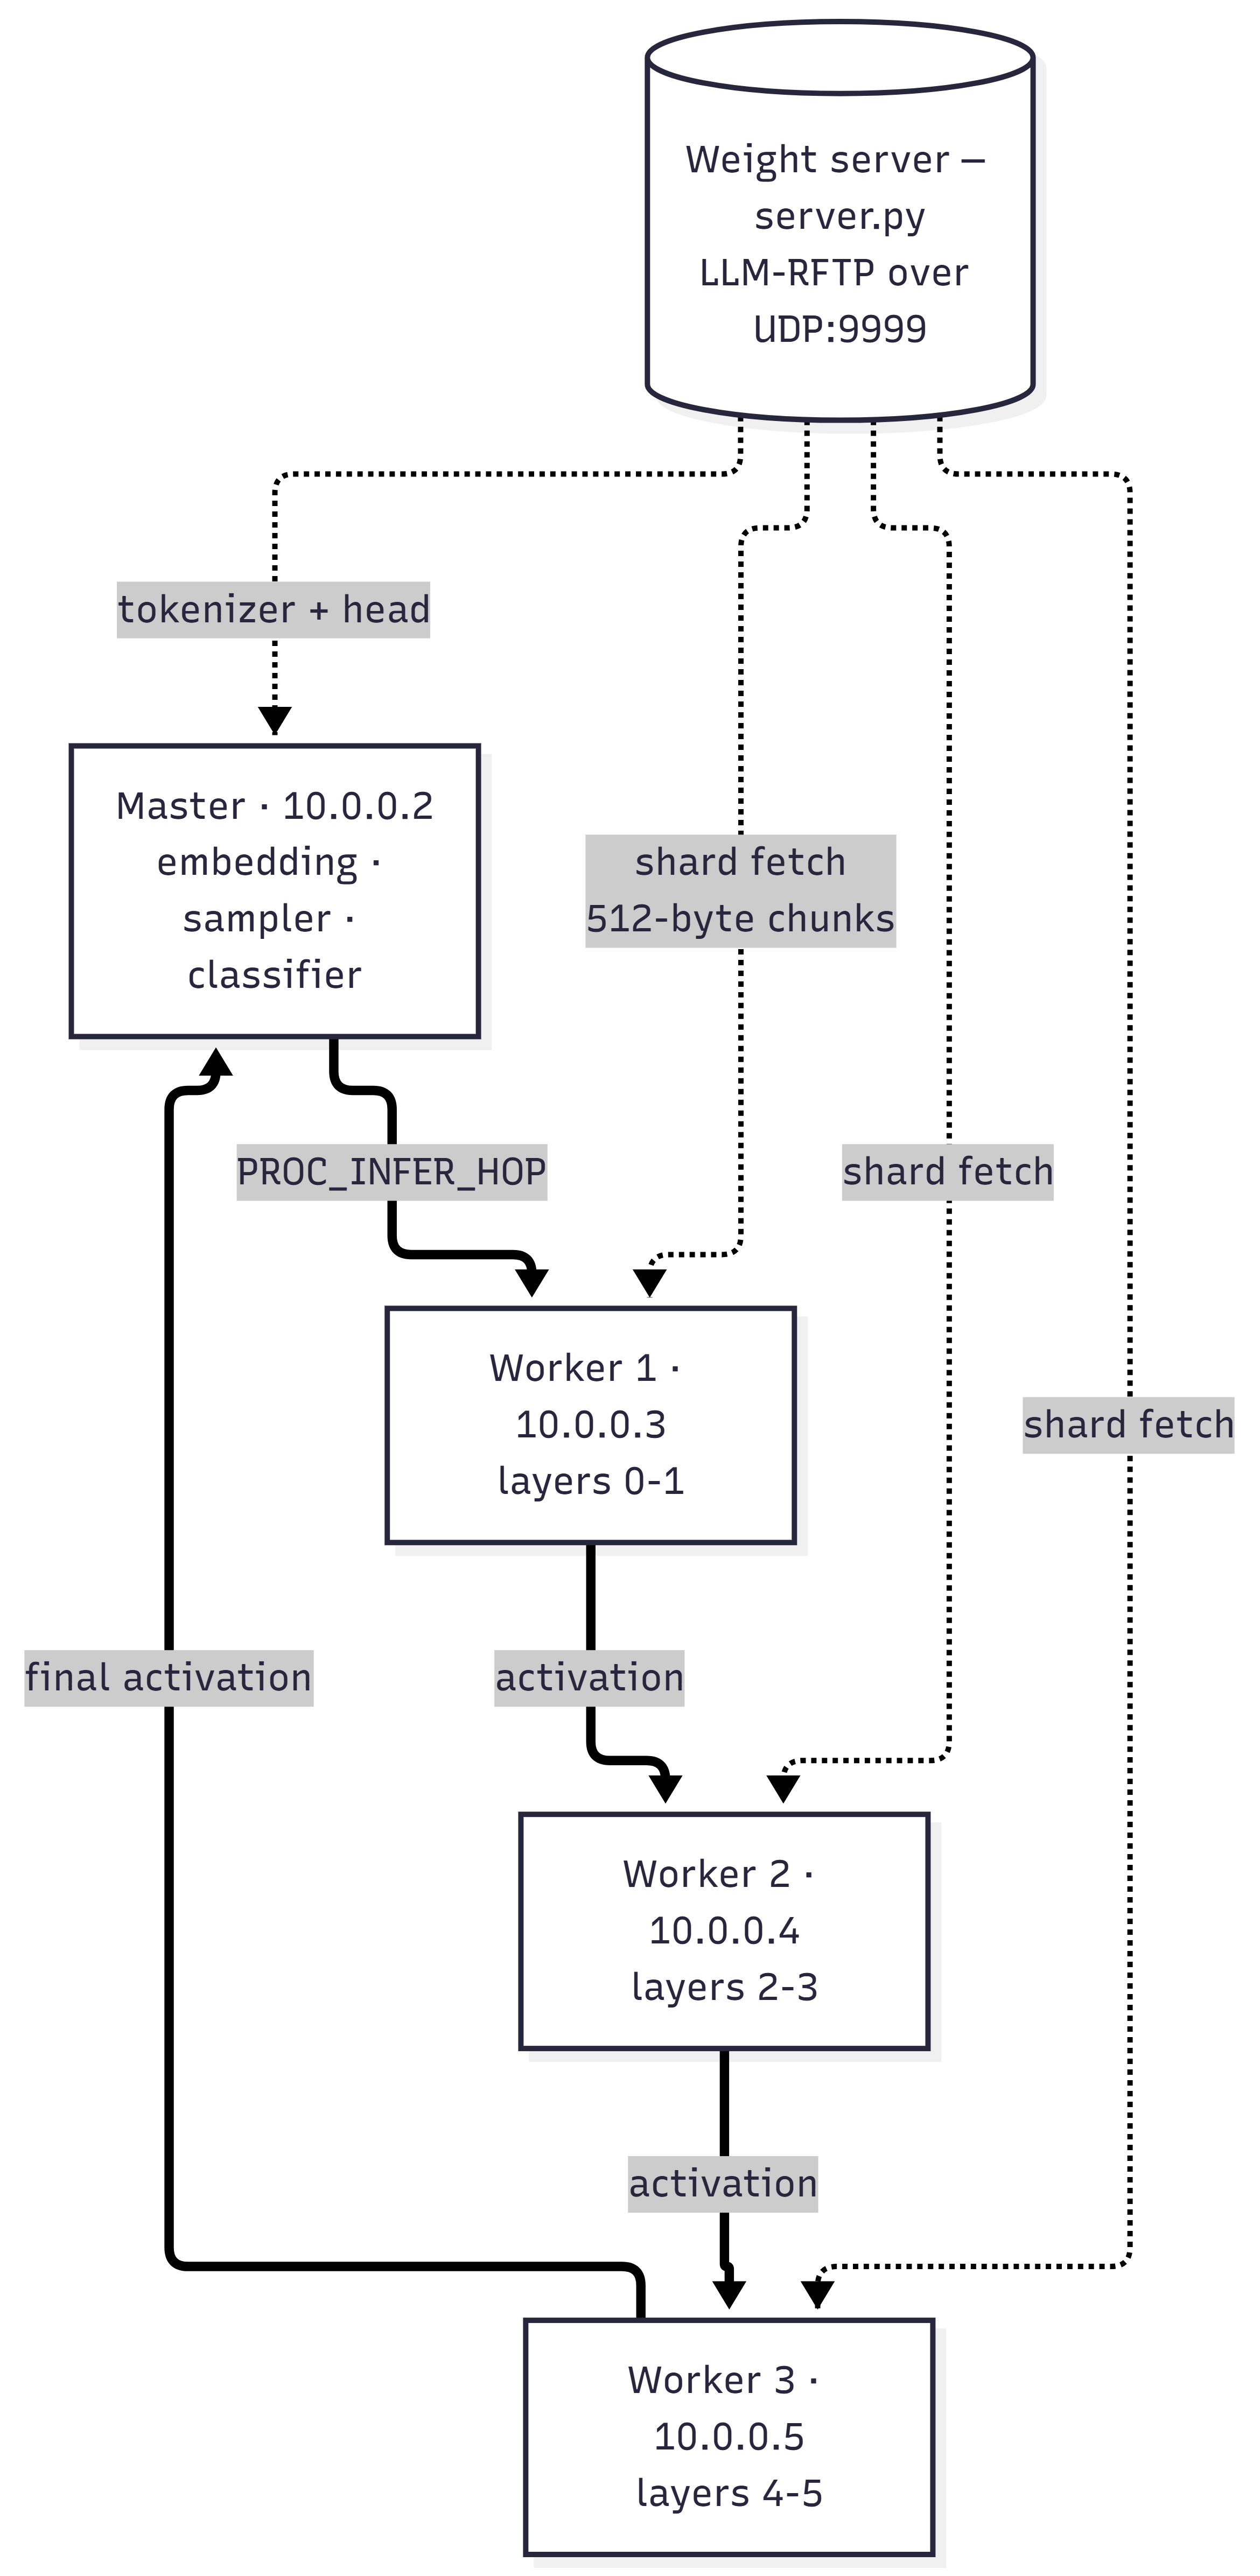
\includegraphics[height=0.50\textheight]{F1-system-architecture.png}
\caption{System architecture: the weight server distributes model checkpoint shards over LLM-RFTP to the master and every worker, while the master and workers form a ring that passes activations by \texttt{PROC\_INFER\_HOP}. The weight server is not part of the ring; it is an ordinary host process reached over the same segment.}
\label{fig:F1}
\end{figure}

\subsection*{F2 --- Wire Format (RPC Envelope + XDR Activation Message)}

\begin{lstlisting}[style=mermaid]
---
config:
  packet:
    bitsPerRow: 16
    bitWidth: 62
    rowHeight: 34
---
packet-beta
title F2 - RPC CALL envelope (RFC 5531) + XDR activation payload
0-3: "XID"
4-7: "mtype = CALL"
8-11: "rpcvers = 2"
12-15: "prog"
16-19: "vers = 1"
20-23: "proc = INFER_HOP"
24-27: "cred flavor = 0"
28-31: "cred len = 0"
32-35: "verf flavor = 0"
36-39: "verf len = 0"
40-67: "infer_hop_t header (7 words)"
68-71: "float[0]"
72-75: "float[1]"
76-79: "float[n-1]"
\end{lstlisting}

\begin{figure}[H]
\centering
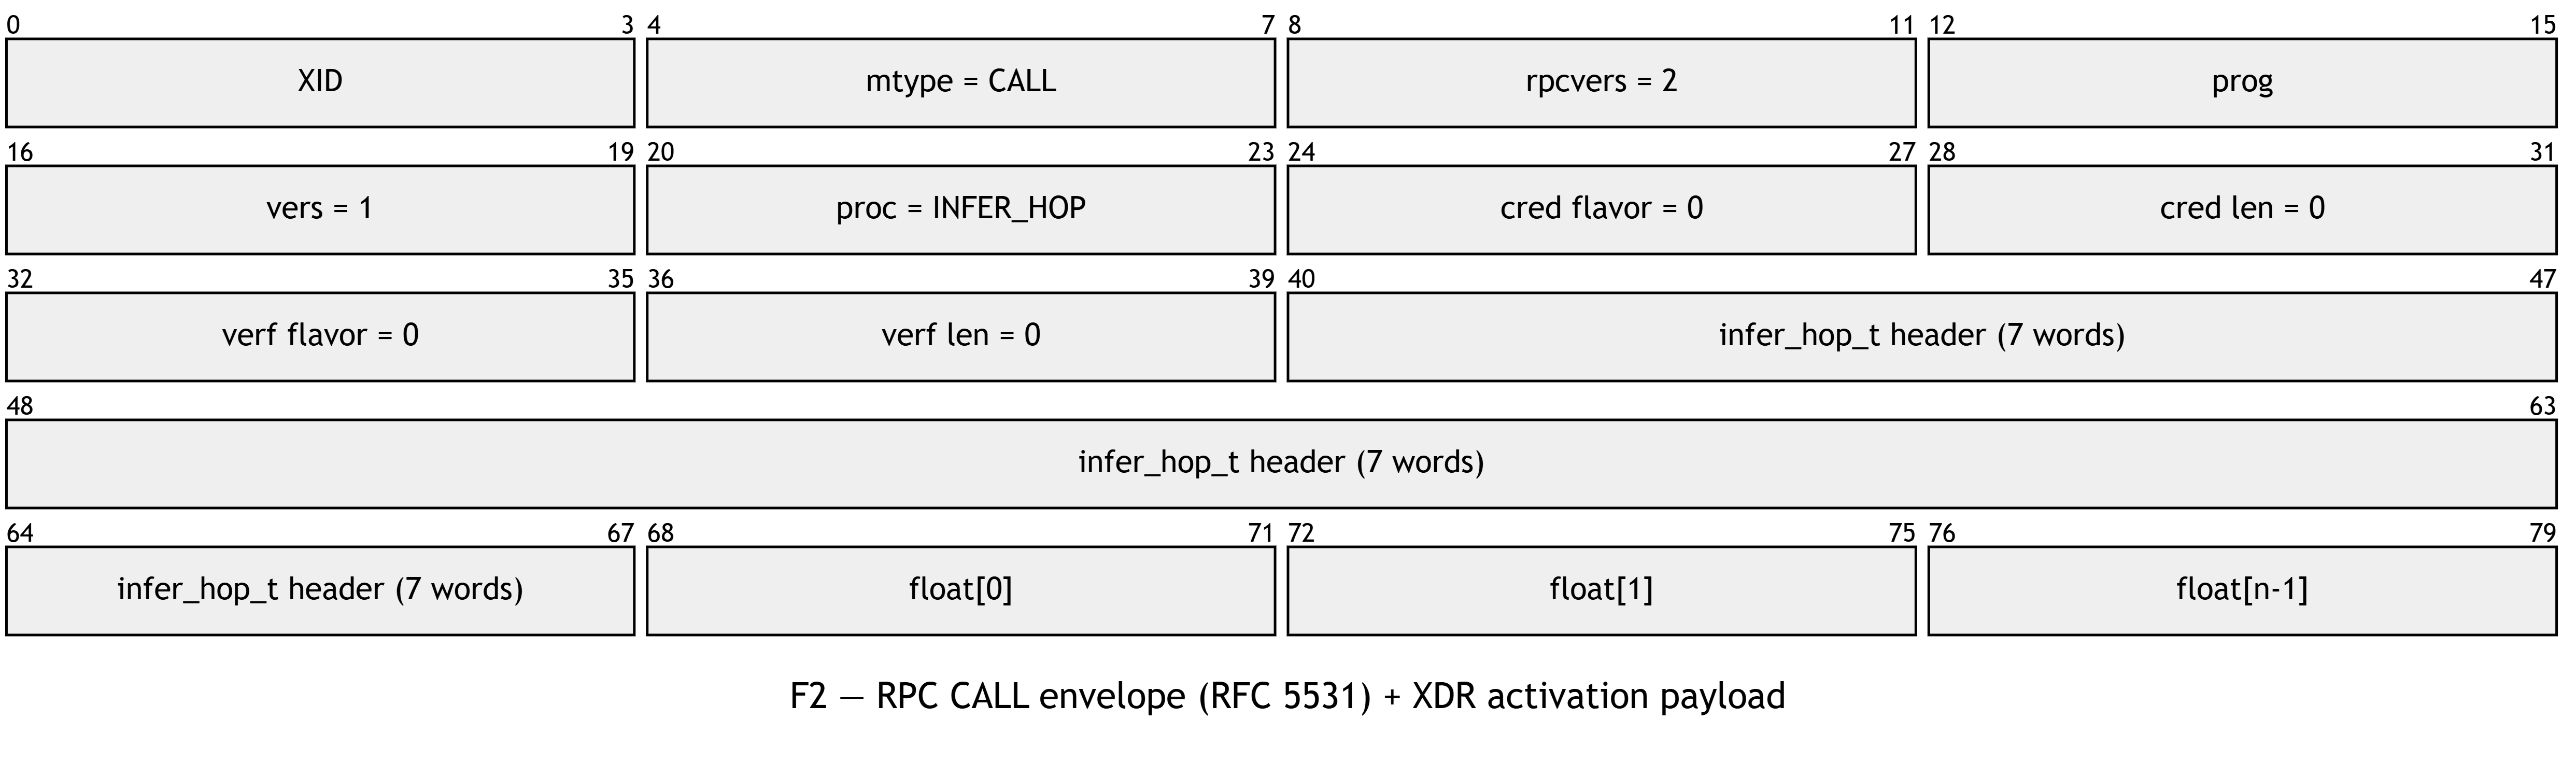
\includegraphics[width=\textwidth]{F2-wire-format.png}
\caption{Wire format of the ONC RPC envelope (RFC 5531) carrying a 7-word \texttt{infer\_hop\_t} header (\texttt{INFER\_HOP\_HDR\_WORDS}, \texttt{user/distinf.h:36}) and the XDR-encoded (RFC 4506) activation array. \texttt{infer\_decode\_hop} (\texttt{user/distinf.c:400--402}) requires \texttt{payload\_len} to equal $28 + 4n$ exactly, \texttt{n\_floats} to be at most \texttt{INFER\_MAX\_FLOATS} (1024), and \texttt{n\_floats} to equal the model's \texttt{dim}.}
\label{fig:F2}
\end{figure}

\subsection*{F3 --- Worker Lifecycle}

\begin{lstlisting}[style=mermaid]
stateDiagram-v2
    [*] --> PENDING: PROC_AUTH_HELLO<br/>(HMAC identity)
    PENDING --> ACTIVE: capability probe answered<br/>(<= 32 MB ceiling)
    ACTIVE --> ACTIVE: PROC_HEARTBEAT<br/>every 200 ticks
    ACTIVE --> SUSPECTED: 2 missed heartbeats<br/>(400 ticks)
    SUSPECTED --> ACTIVE: heartbeat resumes
    SUSPECTED --> EXPIRED: 4 missed heartbeats<br/>(800 ticks)
    EXPIRED --> [*]: evicted, ring re-stitched
\end{lstlisting}

\begin{figure}[H]
\centering
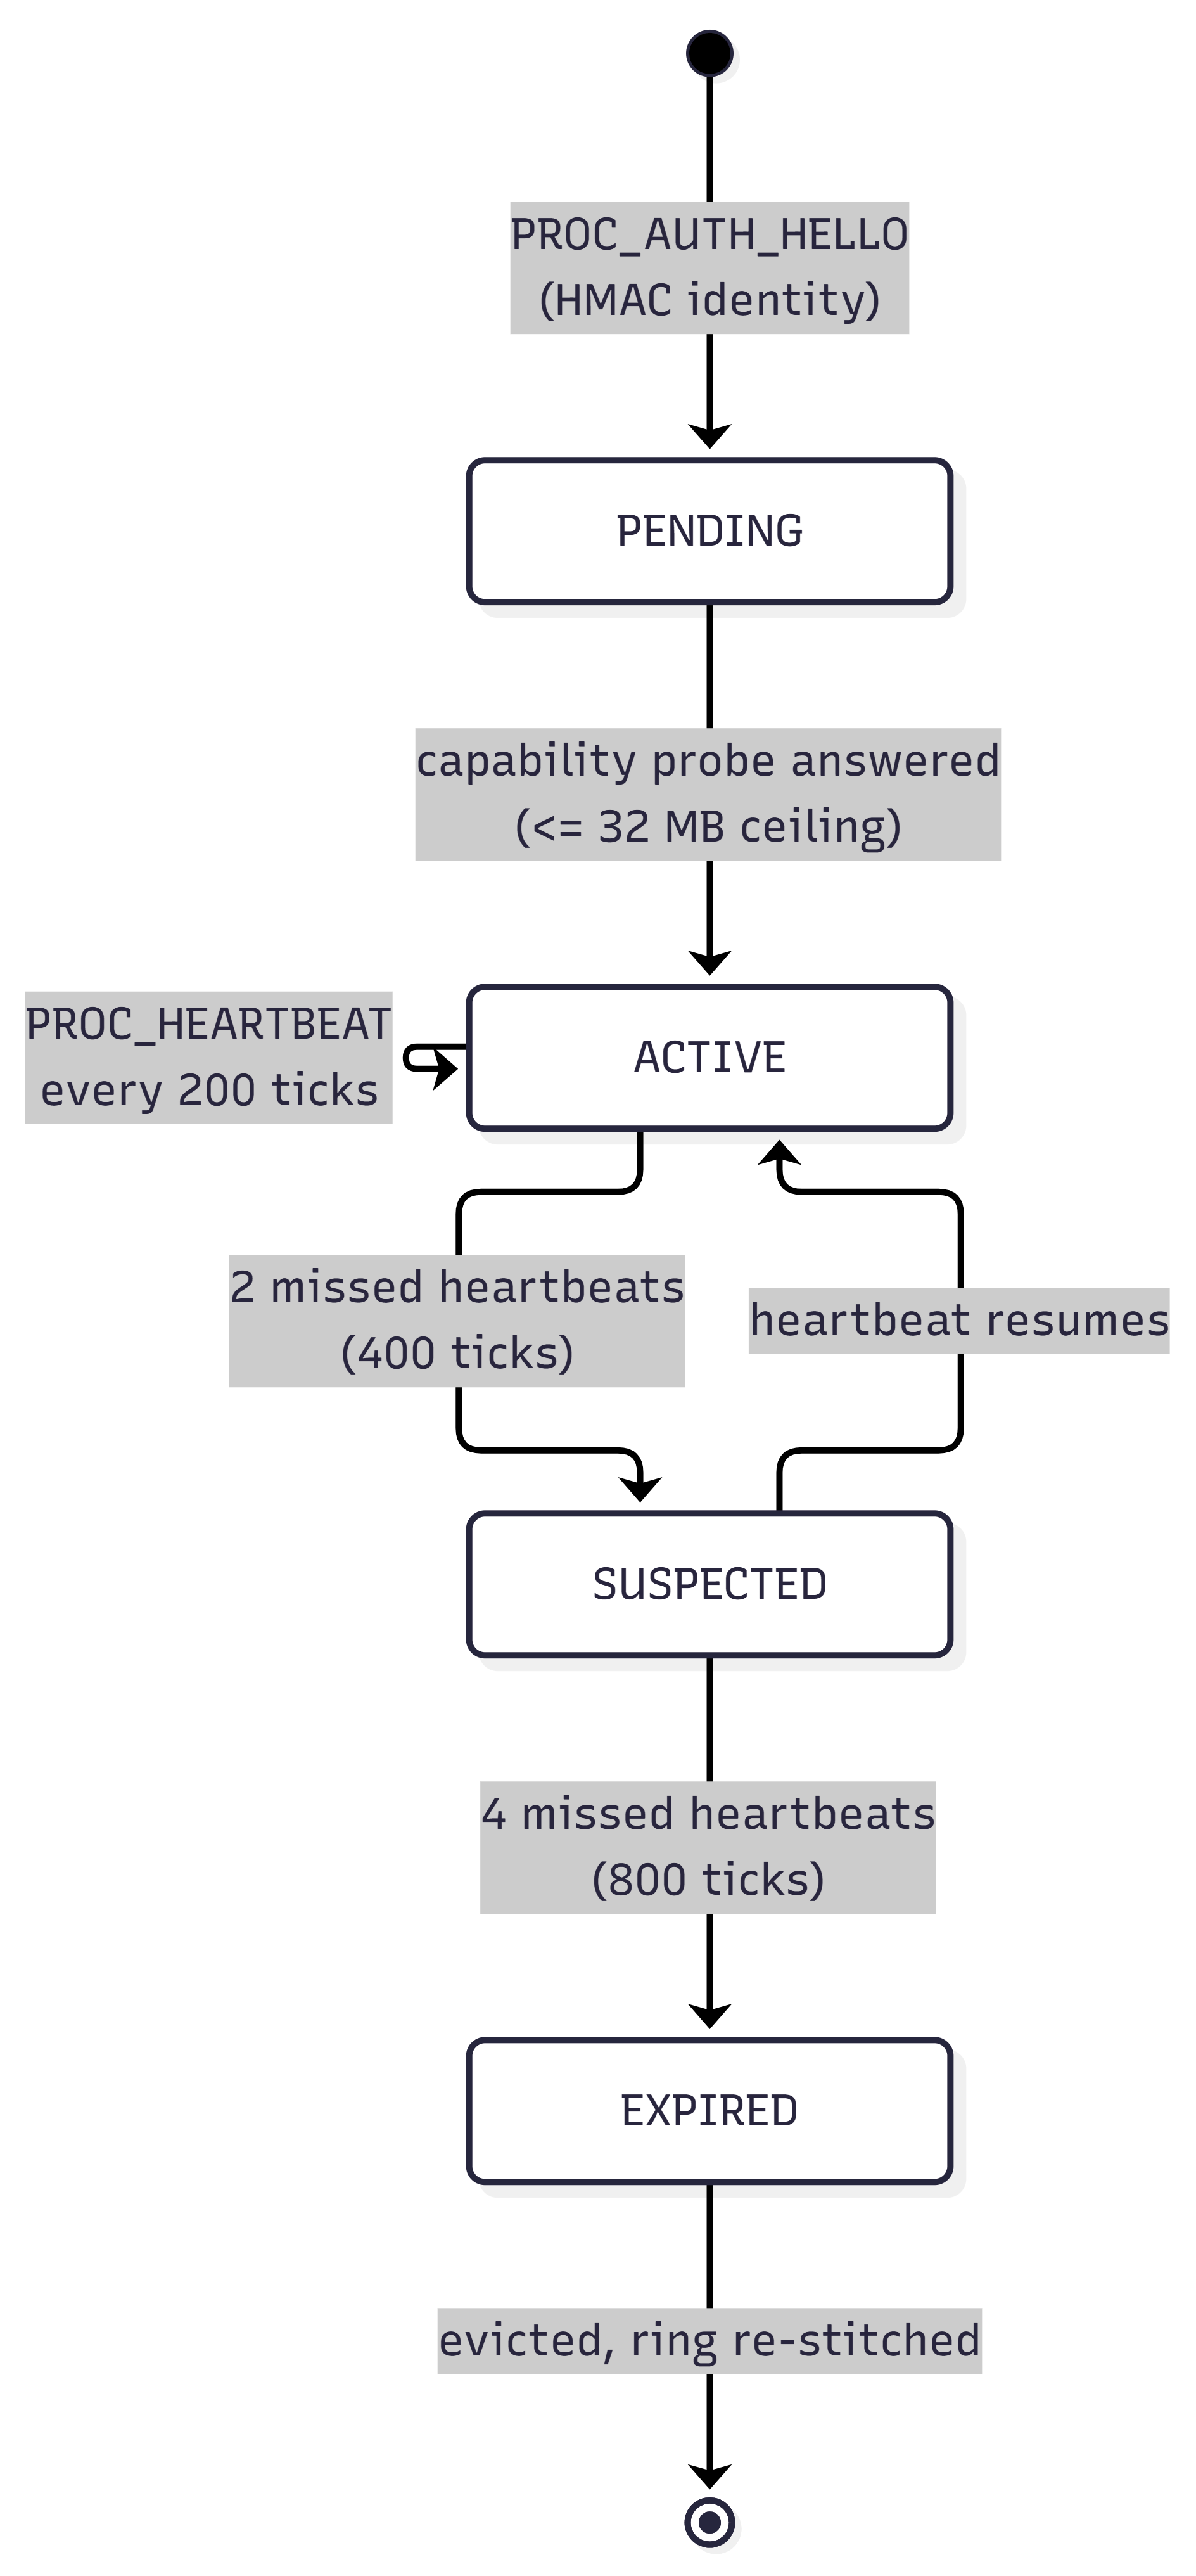
\includegraphics[height=0.50\textheight]{F3-worker-lifecycle.png}
\caption{Worker registration and eviction lifecycle, as implemented in \texttt{user/discovery.c} and \texttt{user/discovery.h}.}
\label{fig:F3}
\end{figure}

\paragraph{Divergence from the existing \texttt{state\_diagram.png}.}
The previous hand-drawn diagram is incorrect because it fails to accurately represent the soft-state lifecycle defined in \texttt{user/discovery.h} and \texttt{user/discovery.c}. Specifically, the code requires a \texttt{PENDING} state in which the node must first answer a sized capability probe before becoming \texttt{ACTIVE}. Furthermore, the code implements intermediate states using specific tick-based timing constants, all defined at \texttt{user/discovery.h:13--25}: \texttt{HEARTBEAT\_INTERVAL\_TICKS} is 200, a worker transitions to \texttt{SUSPECTED} after missing 2 heartbeats (\texttt{HEARTBEAT\_MISS\_SUSPECTED}, 400 ticks), and only transitions to \texttt{EXPIRED} after missing 4 total heartbeats (\texttt{HEARTBEAT\_MISS\_EXPIRED}, 800 ticks), giving it a window to recover. The hand-drawn diagram incorrectly models eviction as an immediate, binary transition, omitting both the \texttt{PENDING} admission state and the \texttt{SUSPECTED} recovery window. The practical consequence is the opposite of what the diagram implies: a node suffering a transient stall rejoins rather than being dropped, which is the entire point of a soft-state registry.

\subsection*{F4 --- Token Sequence}

\begin{lstlisting}[style=mermaid]
sequenceDiagram
    participant M as Master
    participant W1 as Worker 1
    participant W2 as Worker 2
    M->>M: master_run_token() - llama_embed()
    M->>W1: infer_send_hop() [PROC_INFER_HOP]
    W1->>W1: worker_inference_hook()
    W1->>W1: llama_block() x2 layers
    W1->>W2: infer_send_hop()
    W2->>W2: worker_inference_hook()
    W2->>W2: llama_block() x2 layers
    W2->>M: infer_send_hop()
    M->>M: master_handle_final() - llama_head(), sample()
\end{lstlisting}

\begin{figure}[H]
\centering
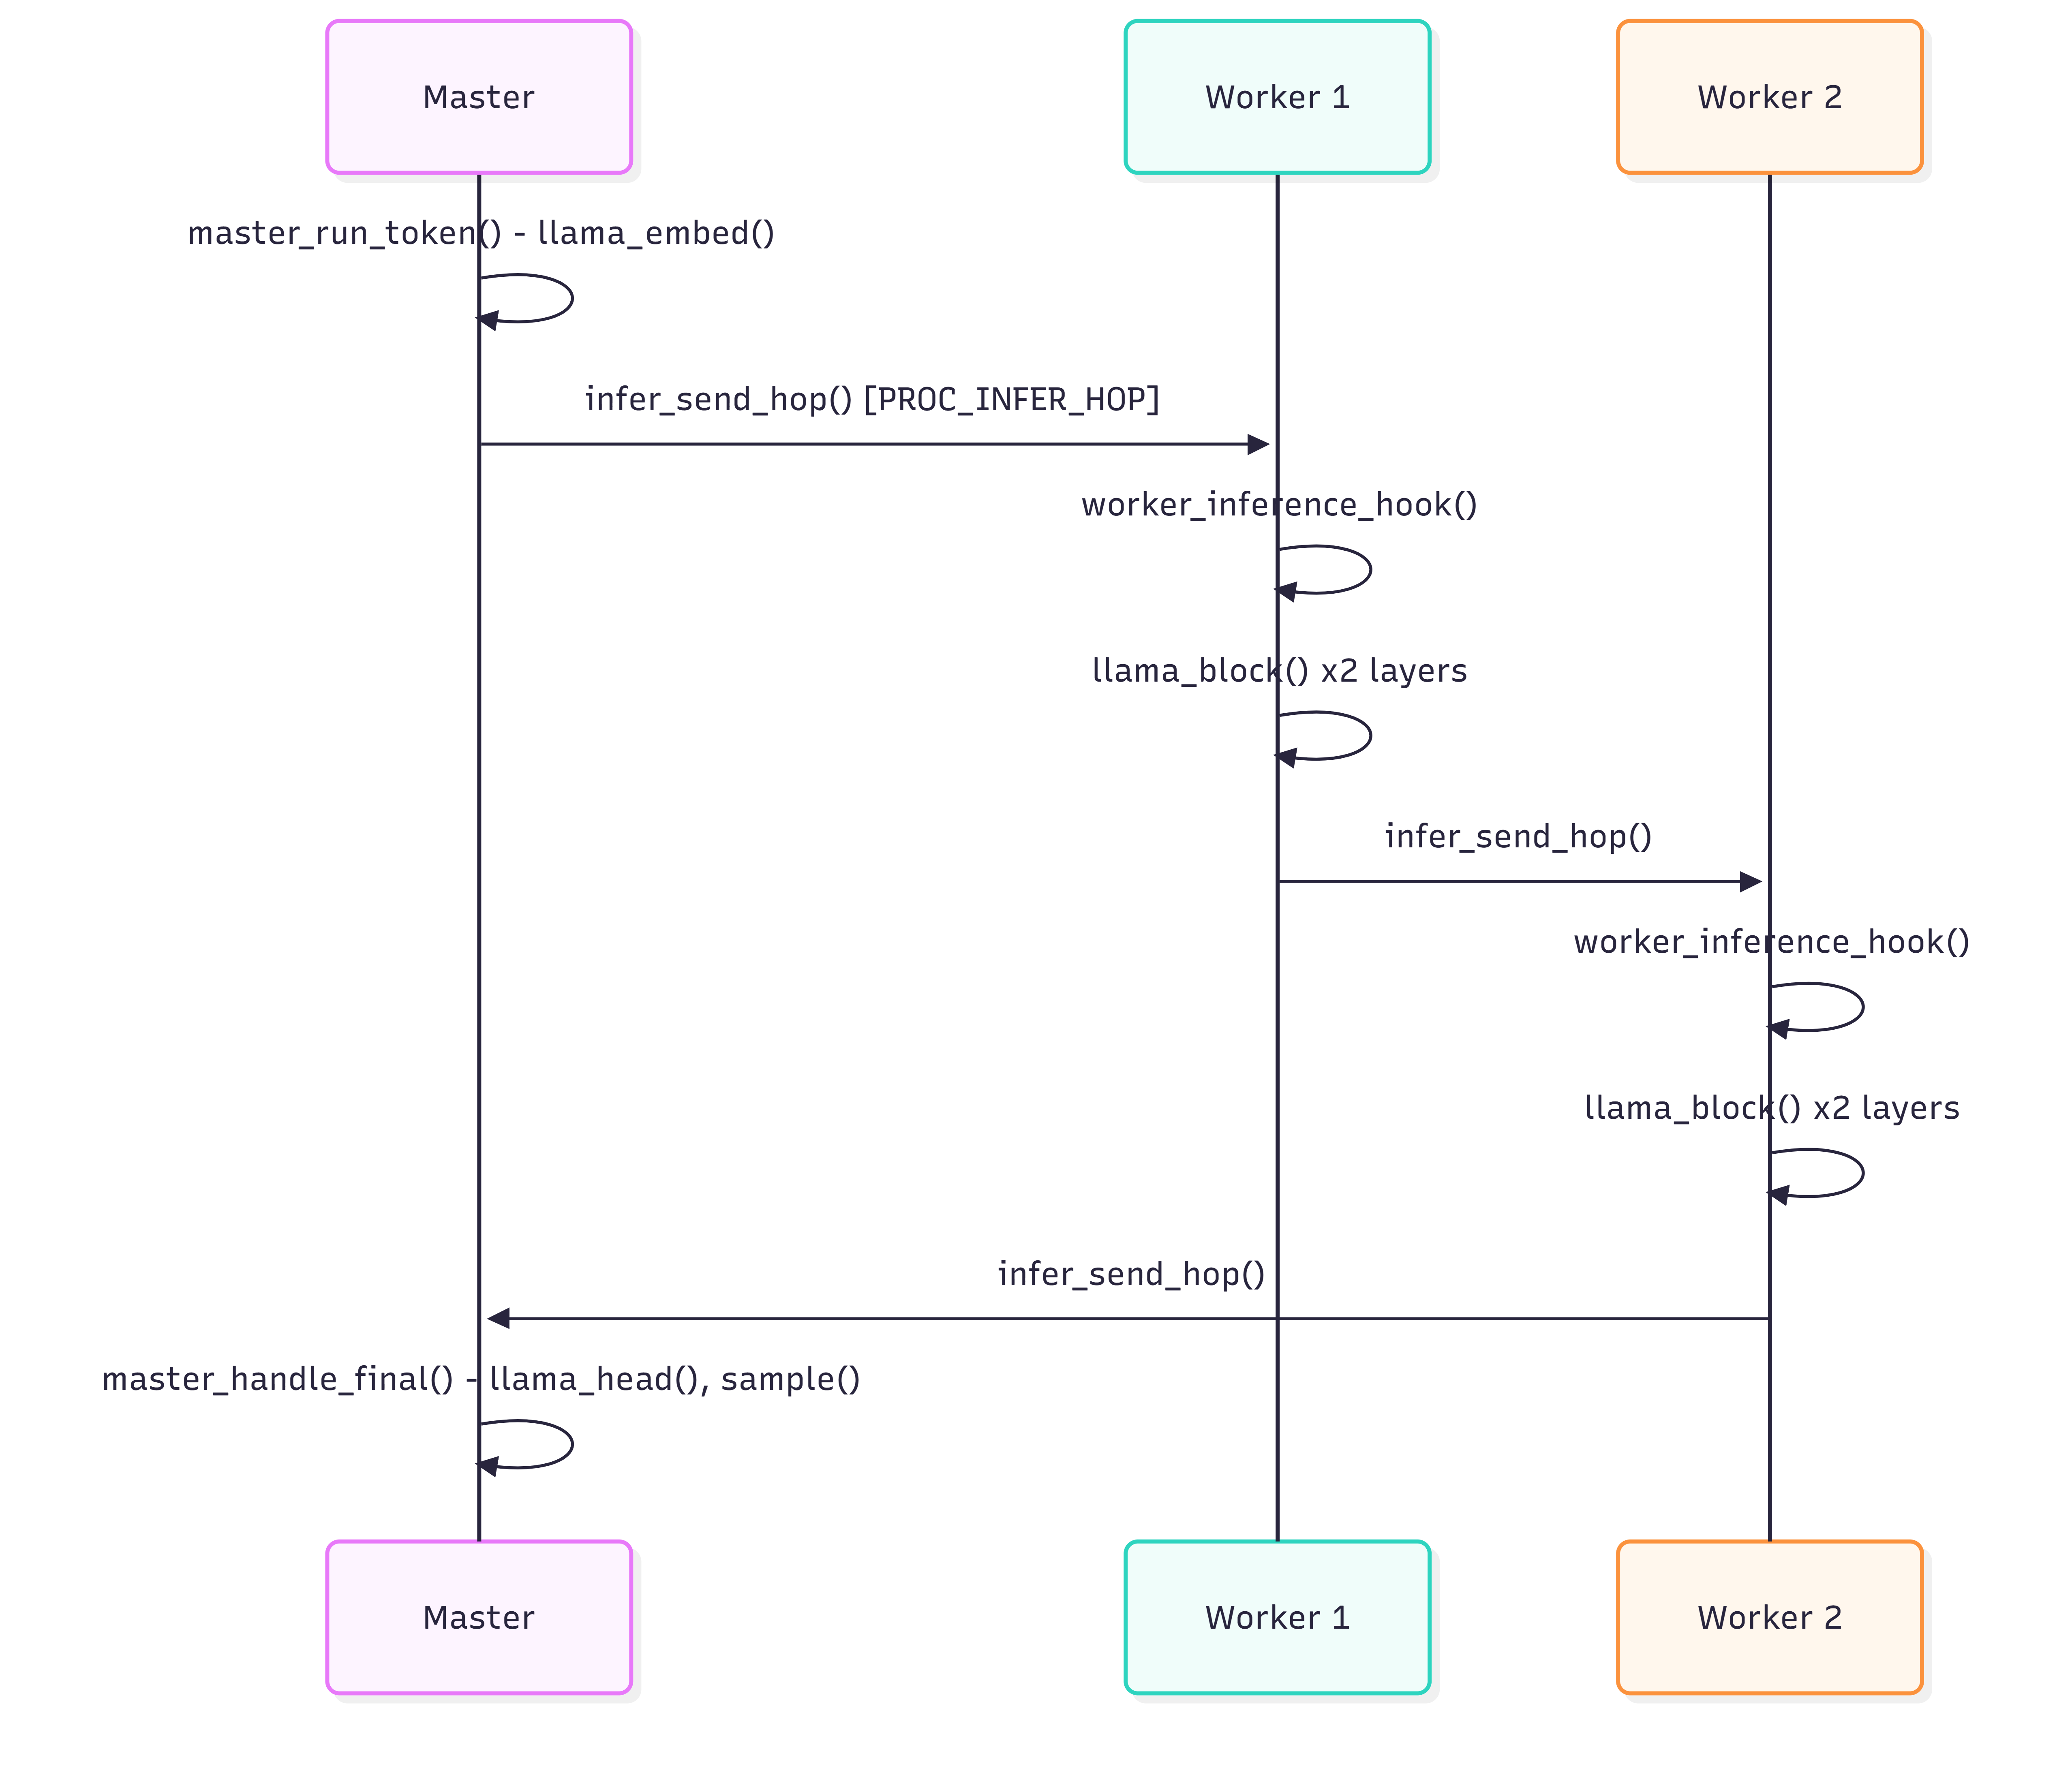
\includegraphics[width=0.82\textwidth]{F4-token-sequence.png}
\caption{One token's round trip through the ring, with the real function names from \texttt{user/distinf.c}: \texttt{infer\_send\_hop} :345, \texttt{worker\_inference\_hook} :605, \texttt{master\_handle\_final} :961, \texttt{master\_run\_token} :1056. Note that a worker runs \texttt{llama\_block} over its own layer range only; \texttt{llama\_embed} and \texttt{llama\_head} belong to the master.}
\label{fig:F4}
\end{figure}

\subsection*{F5 --- Inference Hot Path (\texttt{user/llama\_core.c})}

\begin{lstlisting}[style=mermaid]
flowchart TD
    forward["forward()<br/>llama_core.c:742"] --> llama_embed
    forward --> llama_layer_at["llama_layer_at()<br/>per layer"]
    forward --> llama_block["llama_block()<br/>llama_core.c:653"]
    forward --> llama_head["llama_head()<br/>llama_core.c:732"]
    llama_block --> rmsnorm["rmsnorm() x2"]
    llama_block --> matmul["matmul() x7<br/>wq wk wv wo w1 w3 w2"]
    llama_block --> mha["multihead_attention()<br/>llama_core.c:564"]
    mha --> wda["worker_do_attention()<br/>via thread pool"]
    wda --> softmax
    wda --> dp["dot_product_unrolled()"]
    llama_head --> rmsnorm2["rmsnorm()"]
    llama_head --> matmul2["matmul()"]
\end{lstlisting}

\begin{figure}[H]
\centering
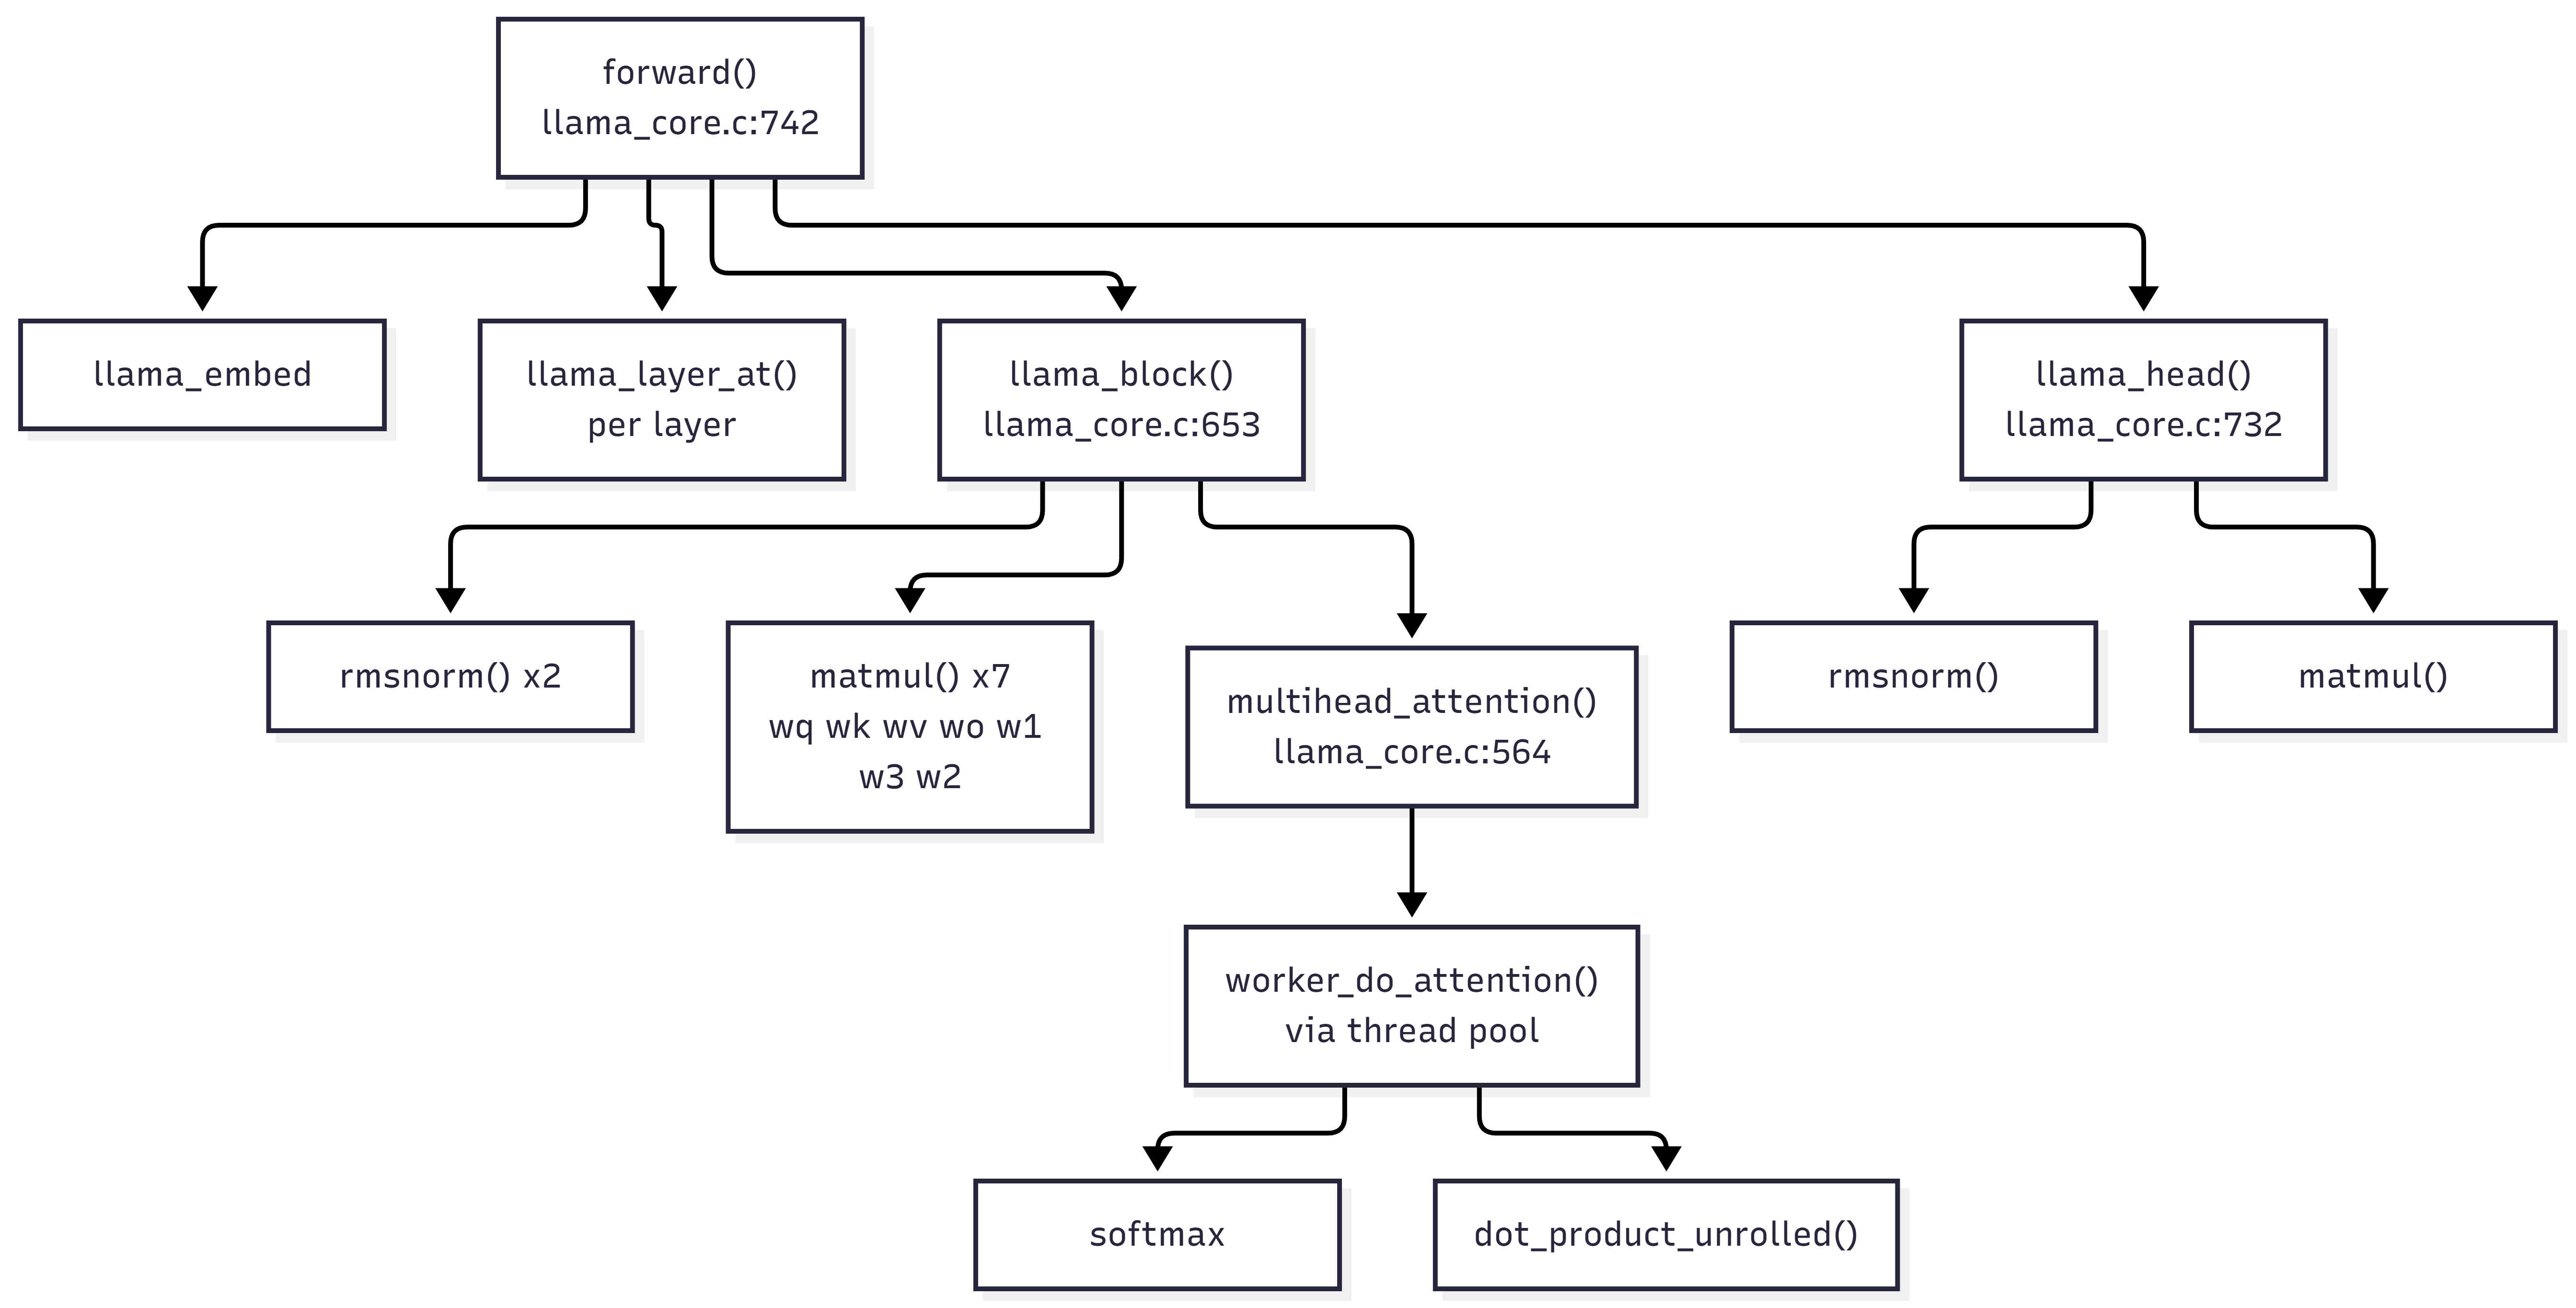
\includegraphics[width=0.88\textwidth]{F5-inference-hot-path.png}
\caption{Call graph through the transformer forward pass in \texttt{user/llama\_core.c}. \texttt{forward} is nine lines long: \texttt{llama\_embed}, then a loop of \texttt{llama\_layer\_at} and \texttt{llama\_block} per layer, then \texttt{llama\_head}. \texttt{multihead\_attention} does \emph{not} call \texttt{matmul}; it dispatches to \texttt{worker\_do\_attention} across the thread pool, where \texttt{softmax} and \texttt{dot\_product\_unrolled} do the work. This is why \texttt{matmul} dominates the profiling table while \texttt{multihead\_attention} appears cheap --- the attention cost is attributed to the pool threads.}
\label{fig:F5}
\end{figure}

\subsection*{F6 --- Node Memory Map}

\begin{lstlisting}[style=mermaid]
block-beta
columns 1
  A["MAXVA - address-space limit"]
  B["TRAMPOLINE = MAXVA - PGSIZE"]
  C["TRAPFRAME = TRAMPOLINE - PGSIZE"]
  D["User stack - canary at s0-56 (observed 0x3fffffbf88)"]
  E["Heap: activations, max 1024 floats per hop"]
  F["Heap: model weights, 60 MB shared-memory segment"]
  G["BSS"]
  H["Data"]
  I["Text - user program base"]
\end{lstlisting}

\begin{figure}[H]
\centering
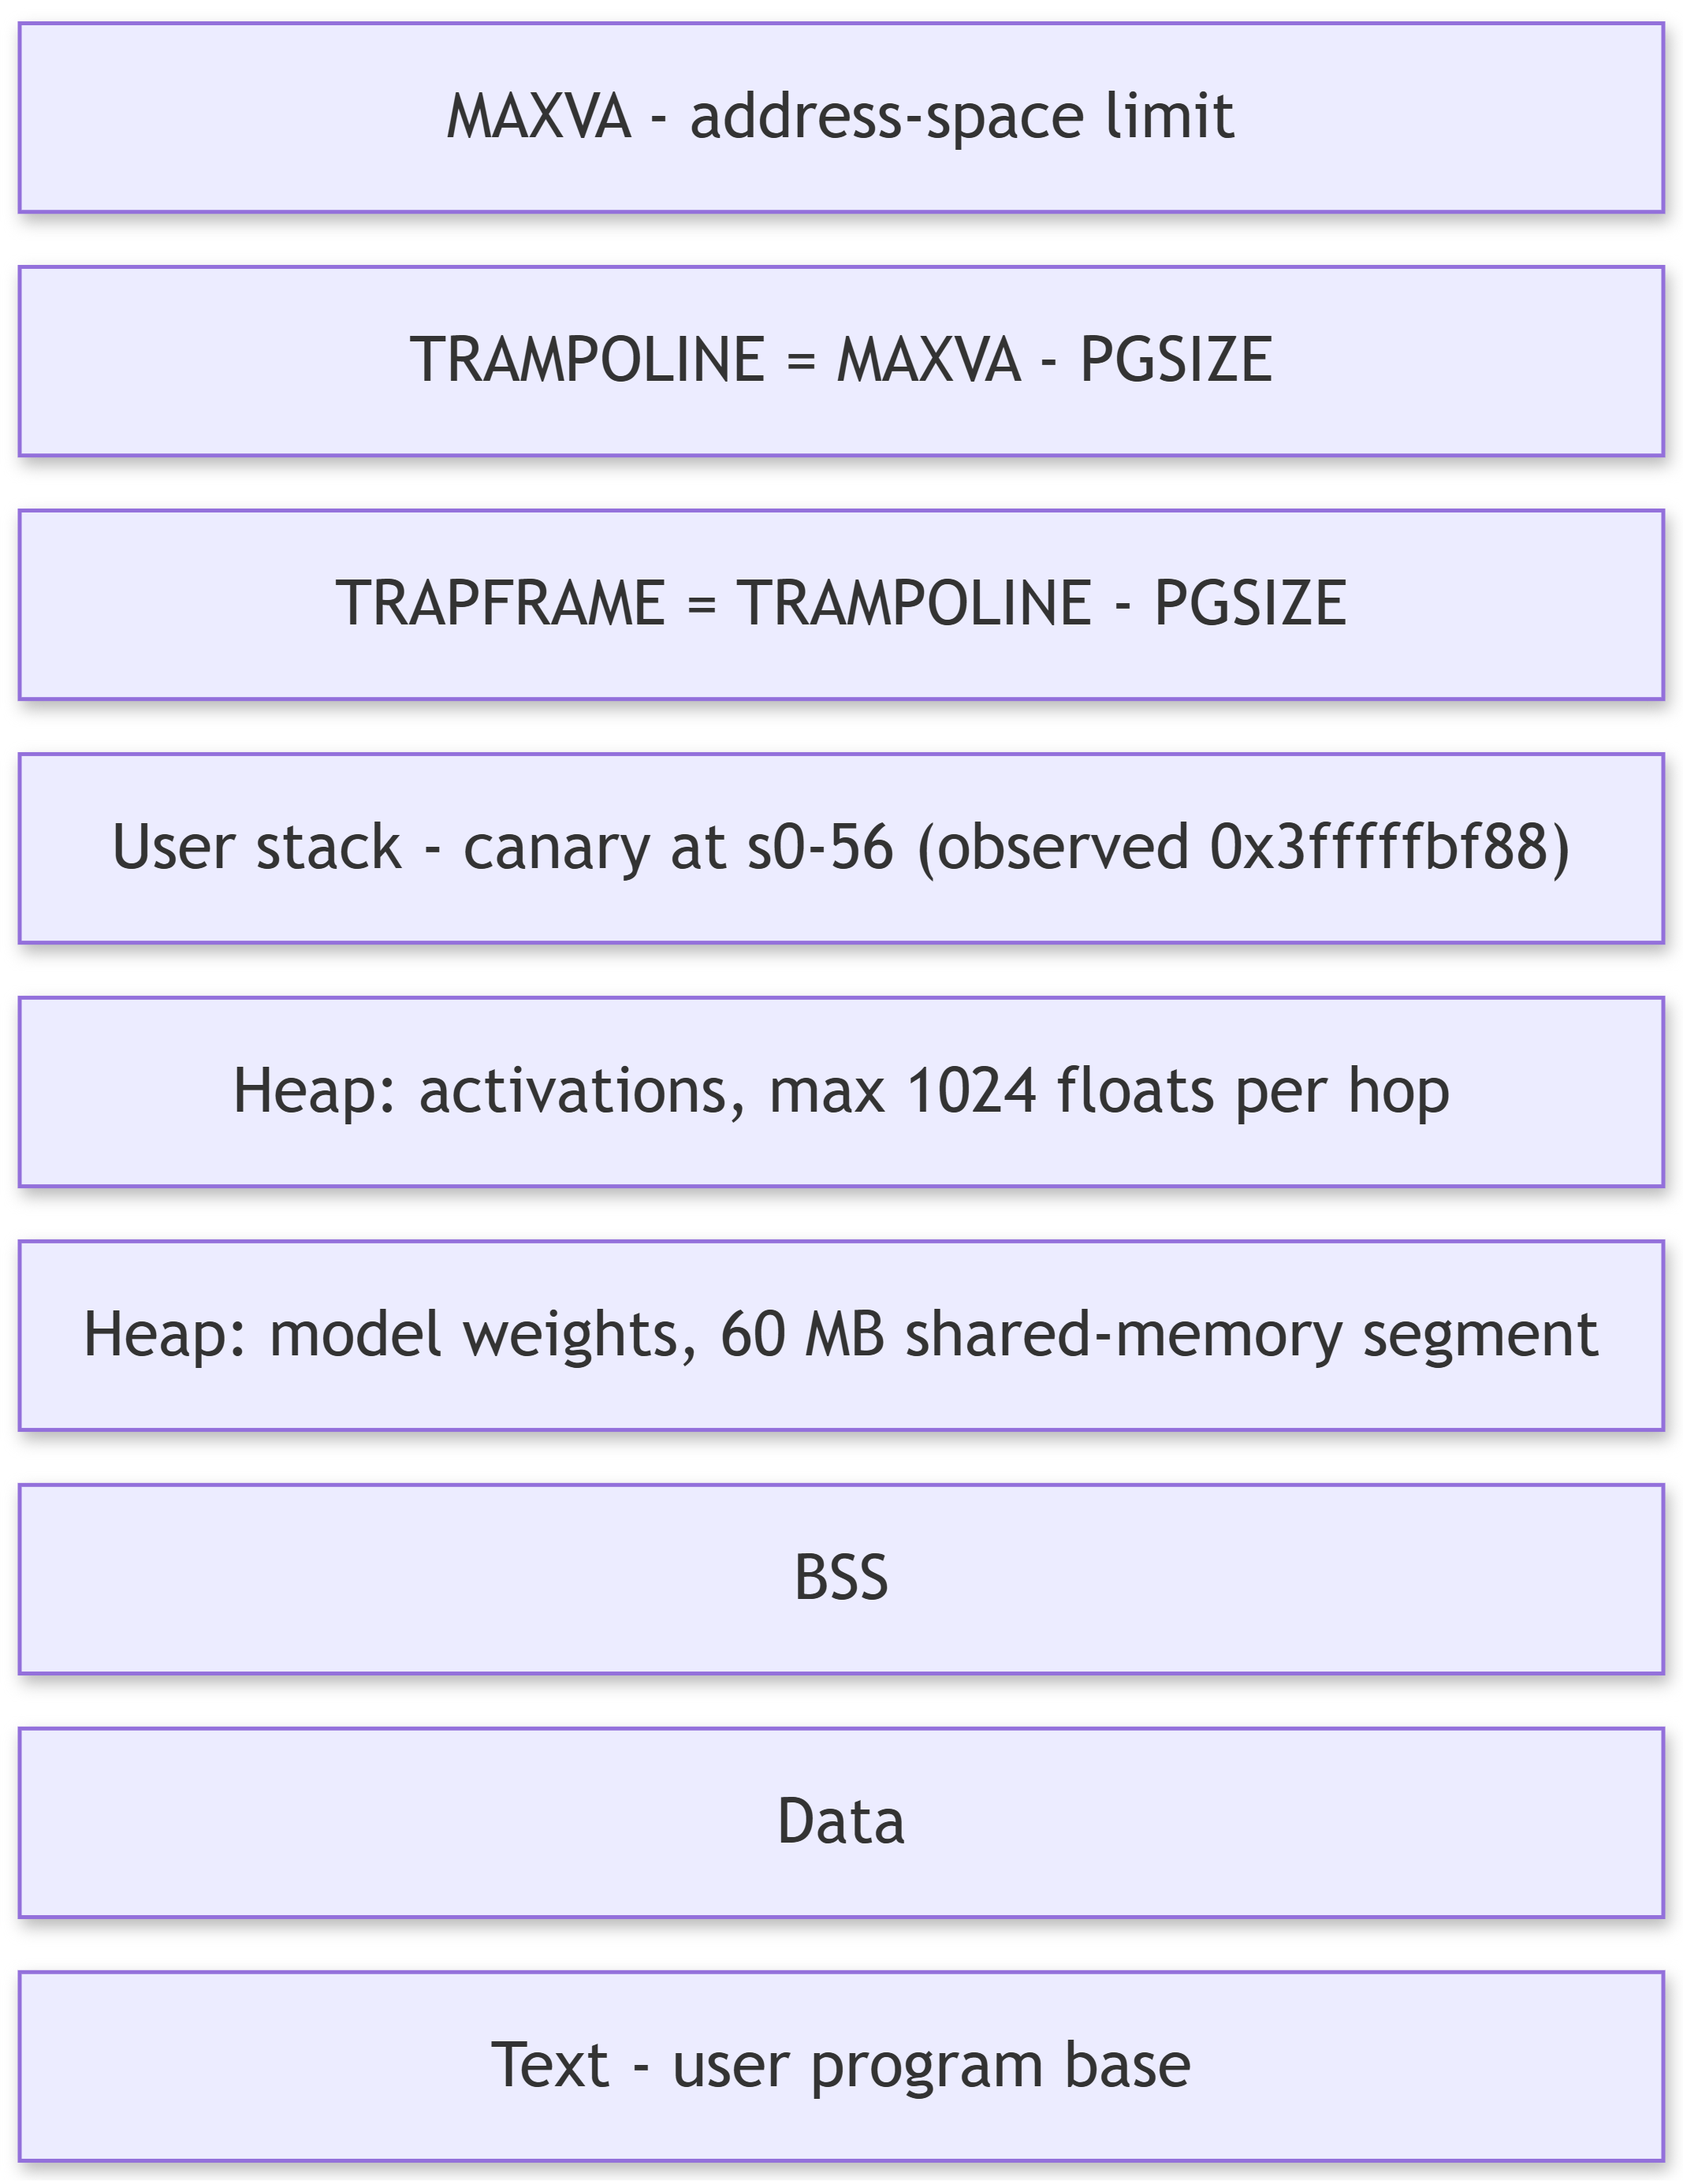
\includegraphics[height=0.46\textheight]{F6-node-memory-map.png}
\caption{Per-node virtual address-space layout: text at the base, then initialised and uninitialised data, the heap (holding the model weights as a shared-memory segment and the per-hop activations), the user stack, the trapframe and trampoline pages, bounded above by \texttt{MAXVA} and the \texttt{RLIMIT\_AS} ceiling. The stack placement is read from the disassembly (\texttt{sd a4,-56(s0)} at \texttt{0x8000584a}) and confirmed live under the debugger.}
\label{fig:F6}
\end{figure}

\subsection*{F7 --- Baseline Graphs}

Two charts, plotting the measurements in Section 3.6.

\begin{lstlisting}[style=mermaid]
xychart-beta
    title "Throughput in tokens/sec (temp 0, 32 steps)"
    x-axis ["SN cold", "SN warm A", "SN warm B", "Ring 2w", "Ring 3w"]
    y-axis "tok/s" 0 --> 5
    bar [3.16, 4.59, 4.70, 0.6, 0.3]
\end{lstlisting}

\begin{figure}[H]
\centering
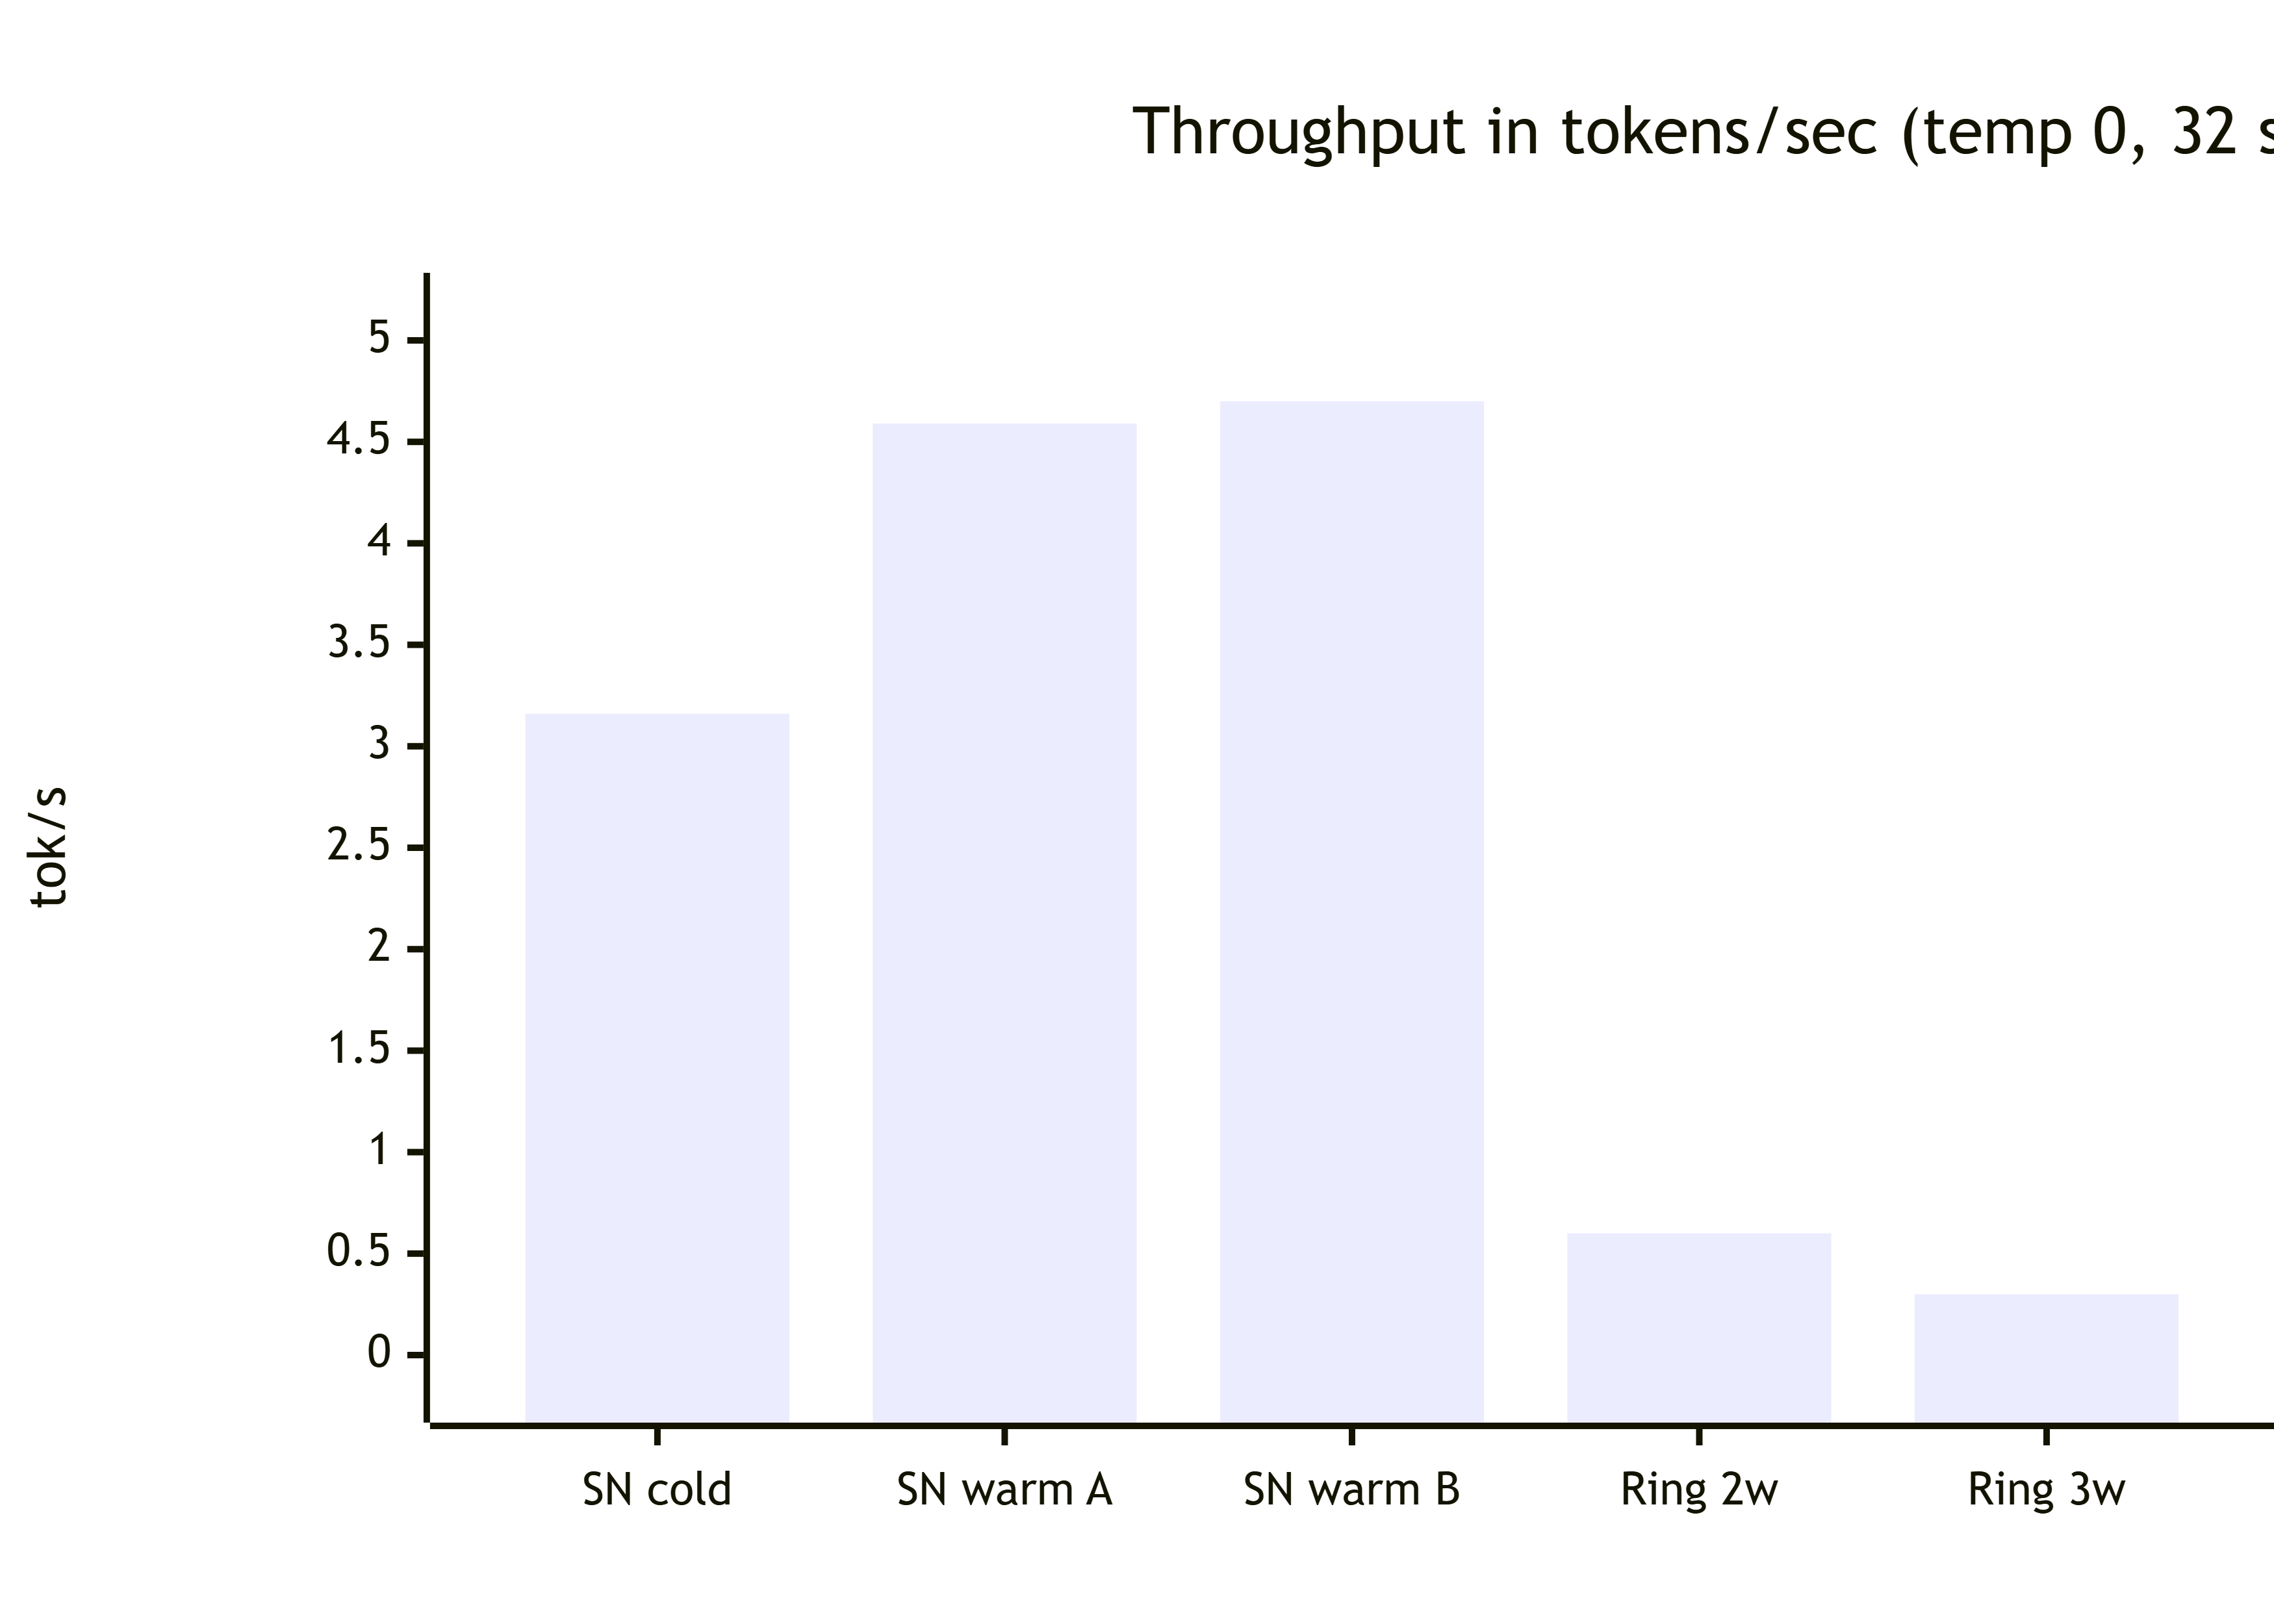
\includegraphics[width=0.70\textwidth]{F7a-throughput.png}
\caption{F7a: throughput across all measured configurations. Distributing the model reduces throughput by roughly an order of magnitude, and adding a third worker halves it again.}
\label{fig:F7a}
\end{figure}

\begin{lstlisting}[style=mermaid]
xychart-beta
    title "Ring per-token latency in milliseconds"
    x-axis ["2w compute", "2w network", "3w compute", "3w network"]
    y-axis "ms" 0 --> 2700
    bar [261, 1193, 394, 2549]
\end{lstlisting}

\begin{figure}[H]
\centering
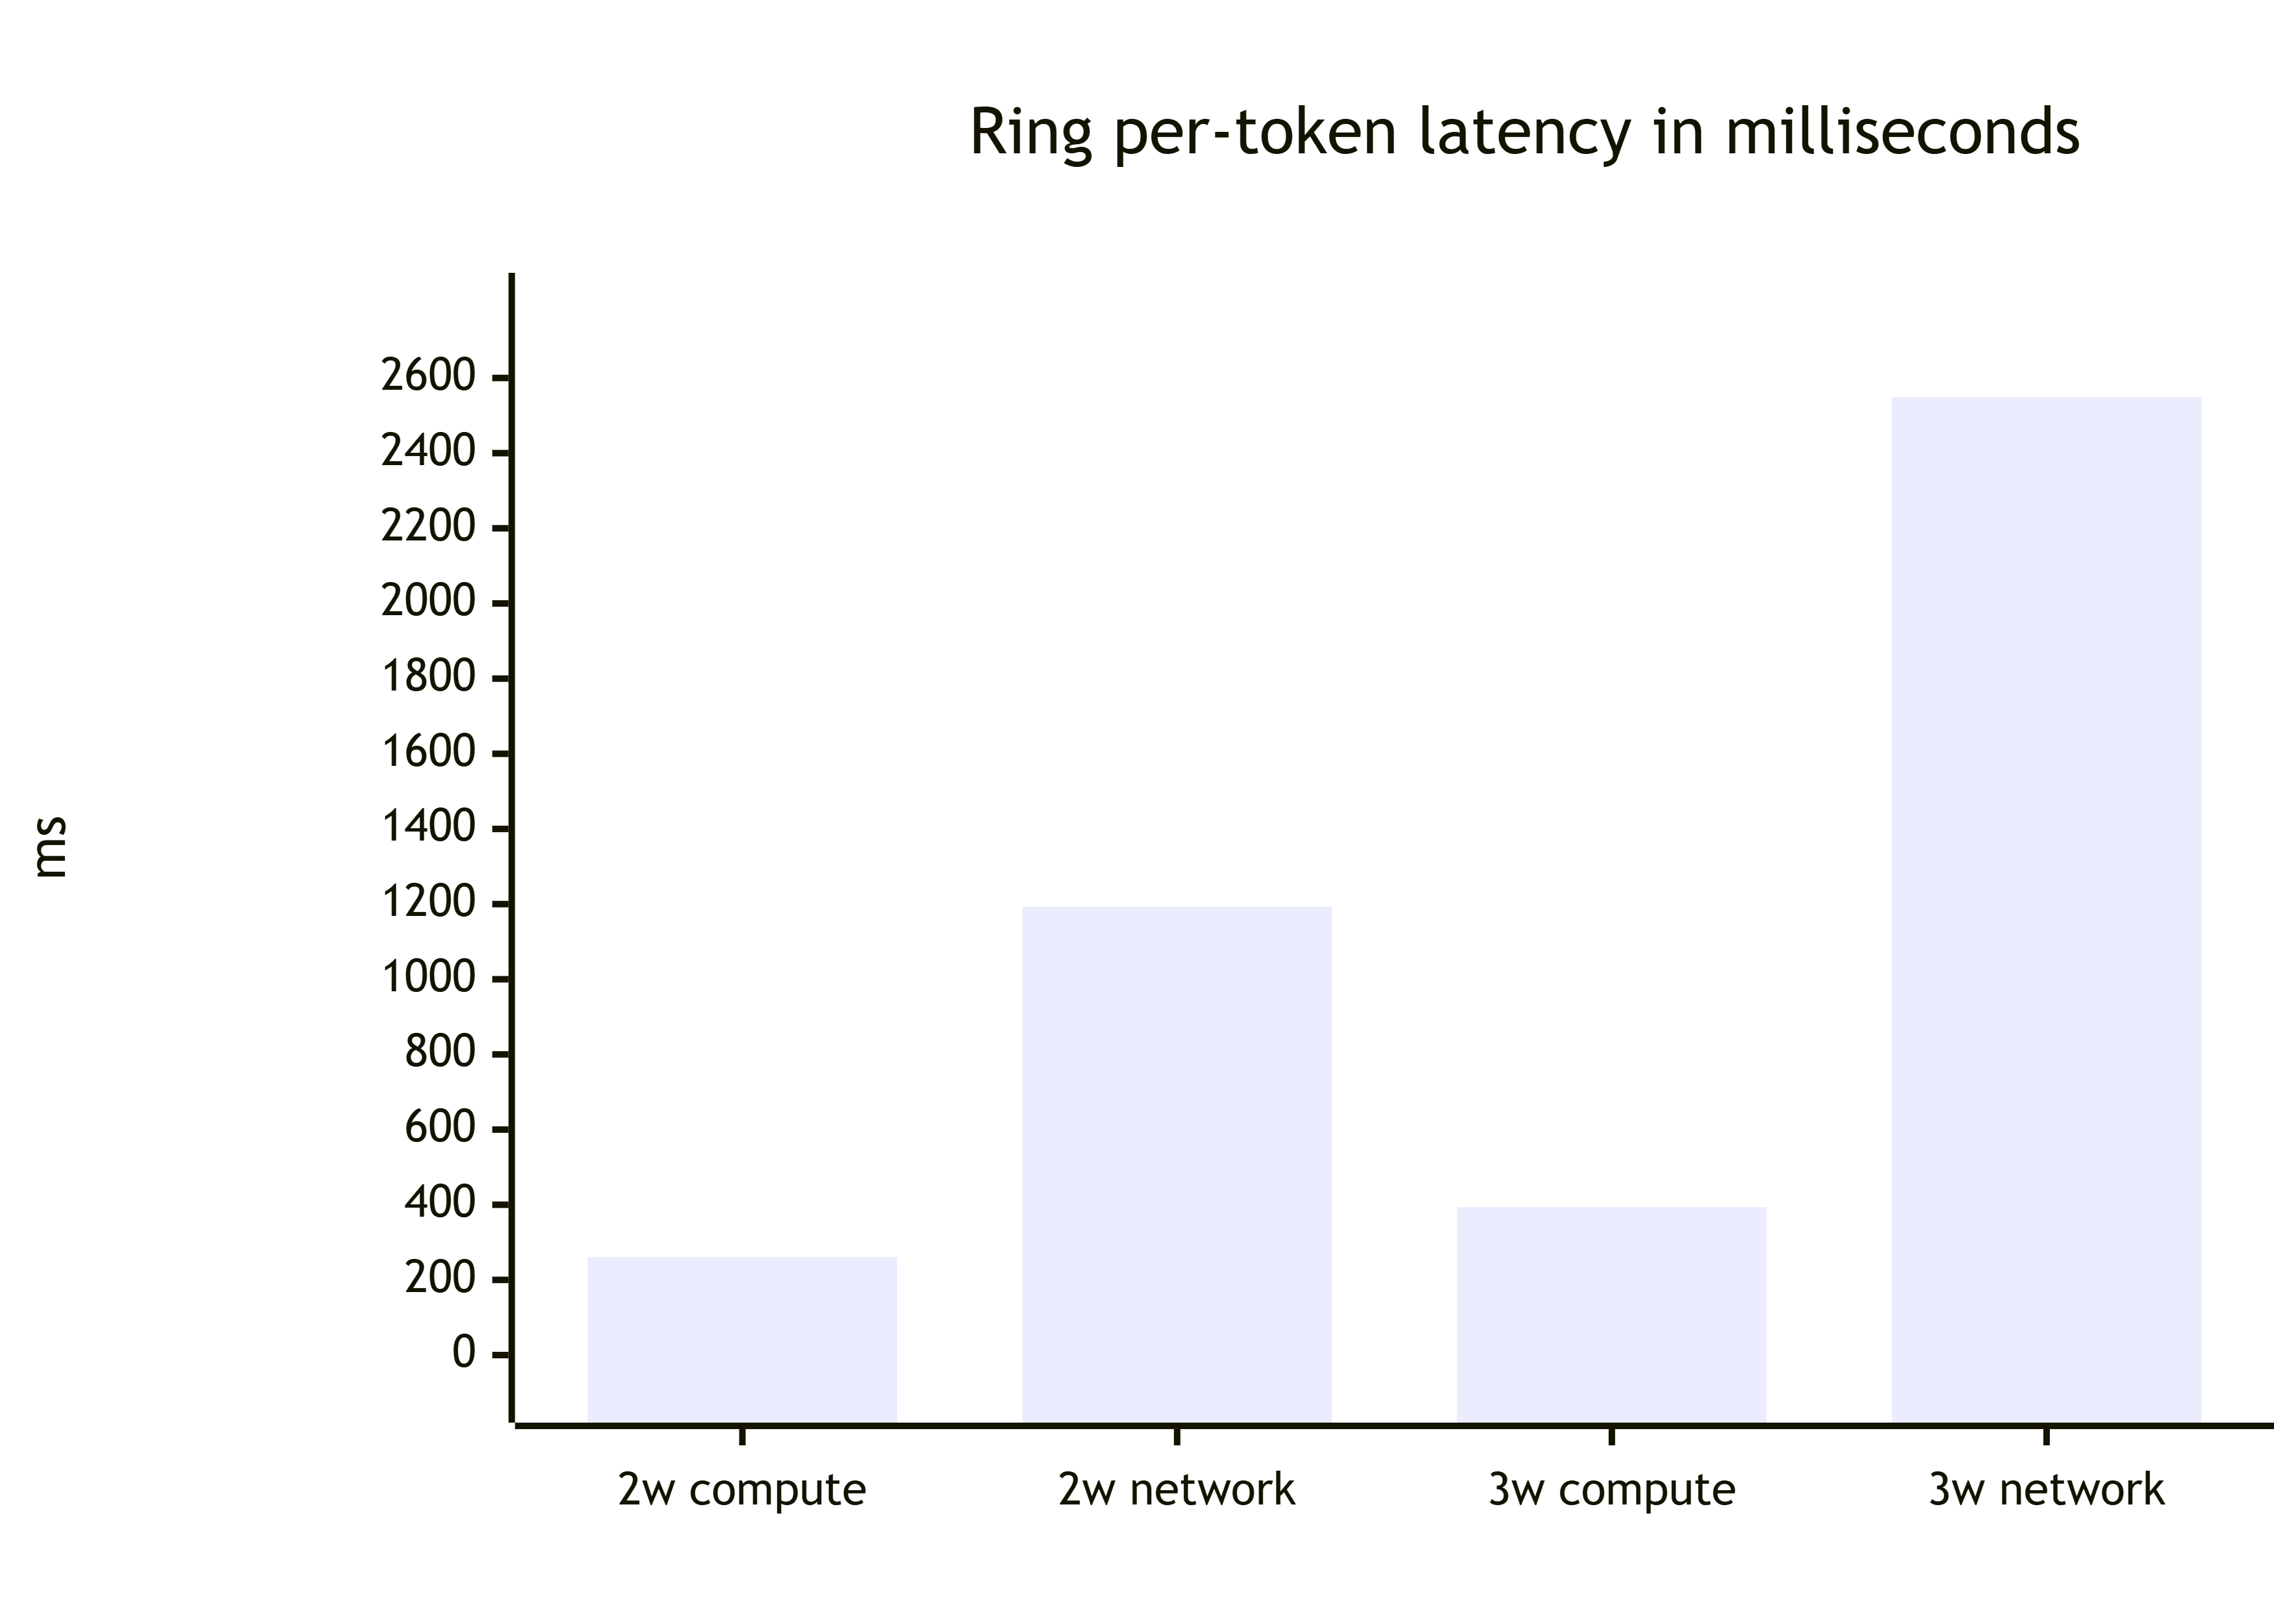
\includegraphics[width=0.70\textwidth]{F7b-latency-split.png}
\caption{F7b: per-token ring latency split into compute and network. The network share rises from 82.0\% at two workers to 86.6\% at three, which is the mechanism behind F7a.}
\label{fig:F7b}
\end{figure}

% =====================================================================
\section*{Section 3.5 --- Difference From Upstream}
\addcontentsline{toc}{section}{Section 3.5 --- Difference From Upstream}
% =====================================================================

Stock xv6-RISC-V has roughly 5,100 lines of kernel source and 21 system calls. \texttt{kernel/syscall.h} in this system declares 59 system call numbers --- 38 above the stock 21. However, only 50 of those 59 are actually implemented in the compiled kernel, so the number of \emph{working} additions is \textbf{29}. The table below records both.

\subsection*{Added System Calls}

\begin{longtable}{@{}R{0.07}R{0.24}R{0.53}R{0.16}@{}}
\toprule
\textbf{\#} & \textbf{System Call} & \textbf{Description} & \textbf{In binary} \\
\midrule
\endhead
22 & \texttt{SYS\_trace} & Traces system calls for process debugging. & \textbf{no} \\
23 & \texttt{SYS\_interpose} & Interposes or hooks into system calls for interception. & \textbf{no} \\
24 & \texttt{SYS\_sigalarm} & Sets up a timer-based signal delivery (alarm). & \textbf{no} \\
25 & \texttt{SYS\_sigreturn} & Returns from a user-space signal handler back to normal execution. & \textbf{no} \\
26 & \texttt{SYS\_symlink} & Creates a symbolic link to a file or directory. & \textbf{no} \\
27 & \texttt{SYS\_mmap} & Maps files or devices into the memory space of a process. & \textbf{no} \\
28 & \texttt{SYS\_munmap} & Unmaps memory previously mapped by \texttt{mmap}. & \textbf{no} \\
29 & \texttt{SYS\_bind} & Binds a network socket to a local port. & \texttt{0x80007f0e} \\
30 & \texttt{SYS\_unbind} & Releases a bound network socket port. & \texttt{0x80007fdc} \\
31 & \texttt{SYS\_send} & Sends a packet over the network. & \texttt{0x80008a10} \\
32 & \texttt{SYS\_recv} & Receives a packet from the network. & \texttt{0x800080d6} \\
33 & \texttt{SYS\_pgpte} & Exposes a single page table entry (debugging/labs). & \textbf{no} \\
34 & \texttt{SYS\_kpgtbl} & Dumps or inspects the kernel page table. & \textbf{no} \\
35 & \texttt{SYS\_shmget} & Allocates a shared memory segment. & \texttt{0x800017f2} \\
36 & \texttt{SYS\_shmat} & Attaches a shared memory segment to the process address space. & \texttt{0x80001864} \\
37 & \texttt{SYS\_shmdt} & Detaches a previously attached shared memory segment. & \texttt{0x800018c6} \\
38 & \texttt{SYS\_shmctl} & Controls or destroys shared memory segments. & \texttt{0x8000190c} \\
39 & \texttt{SYS\_rdcycle} & Reads the RISC-V hardware cycle counter CSR. & \texttt{0x80001506} \\
40 & \texttt{SYS\_rdtime} & Reads the RISC-V hardware timer CSR. & \texttt{0x80001516} \\
41 & \texttt{SYS\_rdinstret} & Reads the RISC-V retired-instruction counter CSR. & \texttt{0x80001526} \\
42 & \texttt{SYS\_getramused} & Returns the total system RAM currently in use. & \texttt{0x8000196e} \\
43 & \texttt{SYS\_setrlimit} & Sets POSIX.1-2017 per-process resource limits. & \texttt{0x80001982} \\
44 & \texttt{SYS\_getrlimit} & Retrieves POSIX.1-2017 per-process resource limits. & \texttt{0x80001a44} \\
45 & \texttt{SYS\_capget} & Retrieves POSIX.1e-style security capabilities. & \texttt{0x80001ac0} \\
46 & \texttt{SYS\_capdrop} & Voluntarily drops POSIX.1e-style capabilities. & \texttt{0x80001ad8} \\
47 & \texttt{SYS\_getentropy} & Retrieves unpredictable random bytes (max 256). & \texttt{0x80001b46} \\
48 & \texttt{SYS\_getuid} & Retrieves the real user identity (POSIX). & \texttt{0x80001c18} \\
49 & \texttt{SYS\_geteuid} & Retrieves the effective user identity. & \texttt{0x80001c30} \\
50 & \texttt{SYS\_setuid} & Sets the real user identity. & \texttt{0x80001c48} \\
51 & \texttt{SYS\_seteuid} & Sets the effective user identity. & \texttt{0x80001cf6} \\
52 & \texttt{SYS\_recvtimeo} & Receives a network packet with a timeout mechanism. & \texttt{0x800082dc} \\
53 & \texttt{SYS\_ip} & Configures or retrieves the node's local IP address. & \texttt{0x80007bc6} \\
54 & \texttt{SYS\_thread\_create} & Creates a new user-level thread. & \texttt{0x80001d90} \\
55 & \texttt{SYS\_thread\_join} & Waits for a user-level thread to terminate. & \texttt{0x80001de4} \\
56 & \texttt{SYS\_thread\_exit} & Terminates the calling user-level thread. & \texttt{0x80001e2a} \\
57 & \texttt{SYS\_yield} & Voluntarily yields the CPU to the scheduler. & \texttt{0x80001e40} \\
58 & \texttt{SYS\_setpriority} & Sets the scheduling priority of a process or thread. & \texttt{0x80001e56} \\
59 & \texttt{SYS\_udp\_bulk} & Declares a bulk UDP flow to bypass token-bucket rate limits (requires \texttt{CAP\_NET\_ADMIN}). & \texttt{0x80008932} \\
\bottomrule
\caption{System calls declared on top of stock xv6 (numbers 22--59), with the address of the handler symbol in the compiled kernel where one exists.}
\label{tab:syscalls}
\end{longtable}

\subsection*{Finding: 59 declared, 50 implemented}

Nine of the declared numbers --- 22--28, 33 and 34 --- have no handler symbol anywhere in the compiled kernel. This is verifiable directly against the symbol table generated in Section 3.2, Phase 4: \texttt{grep sys\_mmap kernel-symbols.txt} returns nothing, while \texttt{grep sys\_setrlimit kernel-symbols.txt} returns \texttt{0x80001982}. The nine absent calls are precisely the MIT 6.828 lab exercises --- syscall tracing, alarm and sigreturn, mmap, symlink and page-table inspection --- carried over as declarations from upstream lab branches that were never merged into this kernel.

The same pattern appears in \texttt{kernel/\allowbreak{}defs.h}, where \texttt{stats.c} (\texttt{statsinit}, \texttt{statsinc}) and \texttt{sprintf.c} (\texttt{snprintf}) are declared behind \texttt{\#ifdef LAB\_LOCK}, and \texttt{vmcopyin.c} (\texttt{copyin\_new}, \texttt{copyinstr\_new}) behind the page-table lab guard. None of their symbols appear in the binary either. \texttt{stats.c} therefore does \emph{not} belong in the file classification below, despite appearing in \texttt{defs.h}.

\subsection*{Classification of Added Files}

\begin{itemize}[leftmargin=3.8cm, labelsep=6pt, itemsep=4pt, font=\normalfont\bfseries]
\item[Networking] \texttt{kernel/net.c}, \texttt{kernel/e1000.c}, \texttt{kernel/pci.c}; \texttt{user/nettest.c}, \texttt{user/netecho.c} --- implements the network stack and hardware drivers.
\item[Distributed Inference] \texttt{user/distinf.c}, \texttt{user/shard.c}, \texttt{user/discovery.c}, \texttt{user/rpc.c}, \texttt{user/xdr.c}, \texttt{user/ftpclient.c}, \texttt{user/shardspike.c} --- implements the node ring, soft-state registry, data serialisation, and model transport.
\item[Model Computation] \texttt{user/llama\_core.c}, \texttt{user/llama.c}, \texttt{user/xmath.c}, \texttt{user/xstdlib.c}, \texttt{user/xstrlib.c}, \texttt{user/sha256.c} --- executes the transformer arithmetic and the freestanding maths and string support it needs.
\item[Hardening] \texttt{kernel/\allowbreak{}stackguard.c}, \texttt{kernel/random.c}, \texttt{kernel/rlimit.h}, \texttt{kernel/\allowbreak{}capability.h}, and the W\^{}X check inside \texttt{kexec}; \texttt{user/\allowbreak{}canarytest.c}, \texttt{user/\allowbreak{}rlimittest.c}, \texttt{user/aslrtest.c}, \texttt{user/wxtest.c}, \texttt{user/wxbad.c}, \texttt{user/idtest.c}, \texttt{user/randtest.c}.
\item[Measurement] \texttt{user/perf.c}, \texttt{user/testperf.c} --- the profiling library and its test harness.
\item[Shared Memory \& Threading] the shared-memory block in \texttt{kernel/\allowbreak{}defs.h} (\texttt{shm\_init}, \texttt{shm\_get}, \texttt{shm\_attach}, \texttt{shm\_detach}, \texttt{shmctl}, \texttt{shm\_cleanup\_proc}), \texttt{kernel/\allowbreak{}shm.h}; \texttt{user/\allowbreak{}testshm.c}, \texttt{user/\allowbreak{}threadtest.c}, \texttt{user/\allowbreak{}threadstack.c}, \texttt{user/mutex.c}, \texttt{user/\allowbreak{}schedtest.c}.
\end{itemize}

\textbf{Shared memory is a sixth category} not named by the assignment, and it is what makes the weight cache work: \texttt{llama} fetches 60~MB once, and later invocations in the same boot attach the existing segment instead of re-fetching. This is visible in our own transcripts, where the first run reports \texttt{Initial 1.7 MB} and subsequent runs report \texttt{Initial 60.2 MB}, and it is the mechanism behind the cold/warm gap analysed in Section 3.6.

% =====================================================================
\section*{Section 3.6 --- Baseline Performance Measurements}
\addcontentsline{toc}{section}{Section 3.6 --- Baseline Performance Measurements}
% =====================================================================

To establish a baseline for single-node inference on the xv6 RISC-V runtime, tests were executed with a single CPU core (\texttt{XV6\_CPUS=1}), a fixed temperature of $T=0$ for deterministic generation, and a generation length of $n = 32$ steps across three distinct prompts. Ring measurements used \texttt{distinf\_sim.py}, which builds its own per-node images.

\subsection*{Method and its limits}

\textbf{Core count.} Single-node runs were taken at \texttt{XV6\_CPUS=1}. \texttt{boot.sh} defaults to three cores, so this must be set explicitly. The absence of the \texttt{hart 1 starting} and \texttt{hart 2 starting} lines in the transcript is the confirmation that it took effect.

\textbf{Timings are relative, not absolute.} QEMU does not model real hardware timing, so guest timings are not real-world timings. The figures below should be read as ratios between configurations rather than as milliseconds on silicon.

\textbf{The counters are not wired into \texttt{llama}, so they were read under the debugger.} The assignment states that the RISC-V counters are ``wrapped by \texttt{user/perf.c}''. Only one of the three is: \texttt{perf.c} calls \texttt{rdtime()} once, at line 260, and converts it to milliseconds. \texttt{rdcycle()} and \texttt{rdinstret()} are declared at \texttt{user/user.h:39--41} and implemented in the kernel (\texttt{sys\_rdcycle} \texttt{0x80001506}, \texttt{sys\_rdinstret} \texttt{0x80001526}), but no file under \texttt{user/} calls either, so a \texttt{llama} run cannot print them and Milestone~1 excludes adding the calls. The counters were therefore read from outside the guest: \texttt{gdb-multiarch} was attached to the QEMU stub, breakpoints were set at the \texttt{sys\_exec} and \texttt{sys\_exit} process boundaries, and the \texttt{\$instret} and \texttt{\$cycle} CSRs were read at each; the difference is the per-process total in Table~\ref{tab:baseline-counters}. The absent user-space caller is recorded in the observations log, and Section 3.9 proposes wiring both counters into \texttt{perf\_metrics} so this measurement is reproducible without a debugger.

\textbf{What the counters actually measure under QEMU.} \texttt{boot.sh} and \texttt{boot-gdb.sh} invoke \texttt{qemu-system-riscv64} without \texttt{-icount}, so QEMU is not counting guest instructions at all; in that mode both the \texttt{instret} and the \texttt{cycle} CSR are derived from the host tick counter rather than from retired instructions and elapsed cycles. This is not an inference from the command line alone --- it was measured directly on an instrumented run, reported below under ``Validating the counters against a run of known duration''. The figures in this section are therefore reported as the assignment directs, as relative quantities for comparing configurations; the IPC column is kept as evidence of the instrument's behaviour, not as a property of the processor.

\textbf{Run-to-run variance is approximately 15\%.} Two runs of the identical two-worker ring configuration produced 0.6 and 0.7 tokens/second, with per-token round-trip times of 1{,}453{,}882 and 1{,}263{,}106 microseconds. All figures below are single-run, and differences smaller than roughly 15\% should not be read as significant.

\subsection*{Single node, three prompts}

\begin{table}[H]
\centering
\small
\begin{tabular}{lrrrrr}
\toprule
\textbf{Prompt} & \textbf{E2EL (ms)} & \textbf{Inference (ms)} & \textbf{TTFT (ms)} & \textbf{tok/s} & \textbf{matmul (ms)} \\
\midrule
``Once upon a time''    & 65{,}145 & 9{,}787 & 56{,}985 & 3.16 & 9{,}663 \\
``The quick brown fox'' &  7{,}213 & 6{,}741 &  1{,}793 & 4.59 & 6{,}630 \\
``In the beginning''    &  7{,}065 & 6{,}589 &  1{,}300 & 4.70 & 6{,}428 \\
\midrule
\textbf{Mean}           & ---      & ---     & ---      & \textbf{4.15} & --- \\
\bottomrule
\end{tabular}
\caption{Single-node baseline over three fixed prompts, 32 steps, temperature 0, \texttt{XV6\_CPUS=1}, all three run in a single boot. 31 tokens were generated in each case.}
\label{tab:baseline-single}
\end{table}

\subsection*{Single node, hardware counters}

\begin{table}[H]
\centering
\small
\begin{tabular}{lrrr}
\toprule
\textbf{Prompt} & \textbf{Instructions retired} & \textbf{Cycles} & \textbf{IPC} \\
\midrule
``Once upon a time''    & 148{,}348{,}807{,}817 & 151{,}378{,}336{,}833 & 0.980 \\
``The quick brown fox'' & 240{,}963{,}933{,}546 & 240{,}546{,}133{,}658 & 1.002 \\
``In the beginning''    &  87{,}822{,}959{,}266 &  86{,}553{,}142{,}387 & 1.015 \\
\midrule
\textbf{Mean}           & 159{,}045{,}233{,}543 & 159{,}492{,}537{,}626 & 0.997 \\
\bottomrule
\end{tabular}
\caption{Counter totals per \texttt{llama} process, read from the \texttt{\$instret} and \texttt{\$cycle} CSRs under \texttt{gdb-multiarch} at the \texttt{sys\_exec} and \texttt{sys\_exit} boundaries. 32 steps, temperature 0, \texttt{XV6\_CPUS=1}, 31 tokens generated in each case. These are a separate set of runs from Table~\ref{tab:baseline-single}, taken in a debugger session rather than a free-running boot, so the two tables are not two views of the same execution. Read as ratios; see the note on what these counters measure under QEMU.}
\label{tab:baseline-counters}
\end{table}

No counter figures were captured for the ring configurations. \texttt{distinf\_sim.py} boots each node itself, so obtaining them would mean attaching a separate debugger to every node in the ring and halting all of them at matching points; the ring is reported on elapsed time alone in Table~\ref{tab:baseline-ring}.

\subsection*{Validating the counters against a run of known duration}

The figures above are only meaningful once it is clear what the counters count. One instrumented run settles it. \texttt{llama} was run on the first prompt under \texttt{gdb-multiarch} with the weight server live, breaking at \texttt{sys\_exec} and again at \texttt{sys\_exit}, so a single execution reports both its own elapsed time and its counter deltas (Figure~\ref{fig:counters-gdb}).

\begin{table}[H]
\centering
\small
\begin{tabular}{lrr}
\toprule
 & \textbf{\texttt{\$instret}} & \textbf{\texttt{\$cycle}} \\
\midrule
At \texttt{sys\_exec} & 321{,}310{,}511{,}864{,}006 & 321{,}315{,}530{,}041{,}607 \\
At \texttt{sys\_exit} & 321{,}570{,}303{,}672{,}917 & 321{,}578{,}004{,}028{,}764 \\
\midrule
\textbf{Delta} & \textbf{259{,}791{,}808{,}911} & \textbf{262{,}473{,}987{,}157} \\
\bottomrule
\end{tabular}
\caption{Counter values at the process boundaries of a single \texttt{llama} run, first prompt, 32 steps, temperature 0, \texttt{XV6\_CPUS=1}. The same run reported \texttt{Total (E2EL) 79808 ms} and 31 tokens at 4.32 tokens/second.}
\label{tab:counter-validation}
\end{table}

Dividing each delta by that run's own elapsed time of 79.808~seconds gives 3.289~GHz for \texttt{\$cycle} and 3.255~GHz for \texttt{\$instret}. Both are the clock rate of the host processor. A counter that returns the host's clock frequency when divided by wall-clock time is measuring host time, not guest work.

Two further details of the same measurement agree. The absolute values are of order $3.2\times10^{14}$, which at that frequency is about 28 hours --- the host machine's uptime, not anything the guest has done, whereas a count of instructions retired by the guest would have begun at zero when xv6 booted. And at each sample \texttt{\$cycle} exceeds \texttt{\$instret} by 5.0 and 7.7 billion ticks, which at 3.289~GHz is 1.5 and 2.3 seconds: the interval between typing the two \texttt{gdb} commands. Two independent counters do not drift apart by exactly the operator's typing speed.

The consequence is bounded, and worth stating plainly. The figures remain valid as relative measures --- a configuration that takes longer registers proportionally more, so ratios between configurations hold, which is what this section is asked to report. They are not instruction counts, and the IPC column is an artefact of sampling one clock twice rather than a property of the processor. The same conclusion follows from the other direction: the delta above divided by the 31 tokens generated is $8.4\times10^{9}$ ``instructions'' per token, for a 15M-parameter model whose forward pass is on the order of $3\times10^{7}$ arithmetic operations --- two orders of magnitude too large.

\begin{figure}[H]
\centering
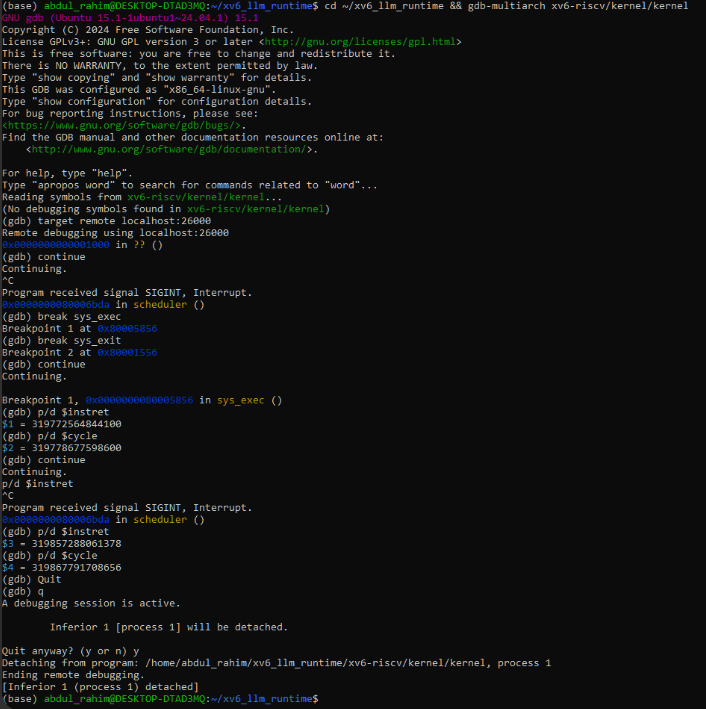
\includegraphics[width=0.92\textwidth]{M1-3.6-05-counters-gdb.png}
\caption{The instrumented run. Breakpoint~1 is hit twice --- once as \texttt{init} execs \texttt{sh}, once as \texttt{sh} execs \texttt{llama} --- and the counters are read at the second hit and again at \texttt{sys\_exit}.}
\label{fig:counters-gdb}
\end{figure}


\begin{figure}[H]
\centering
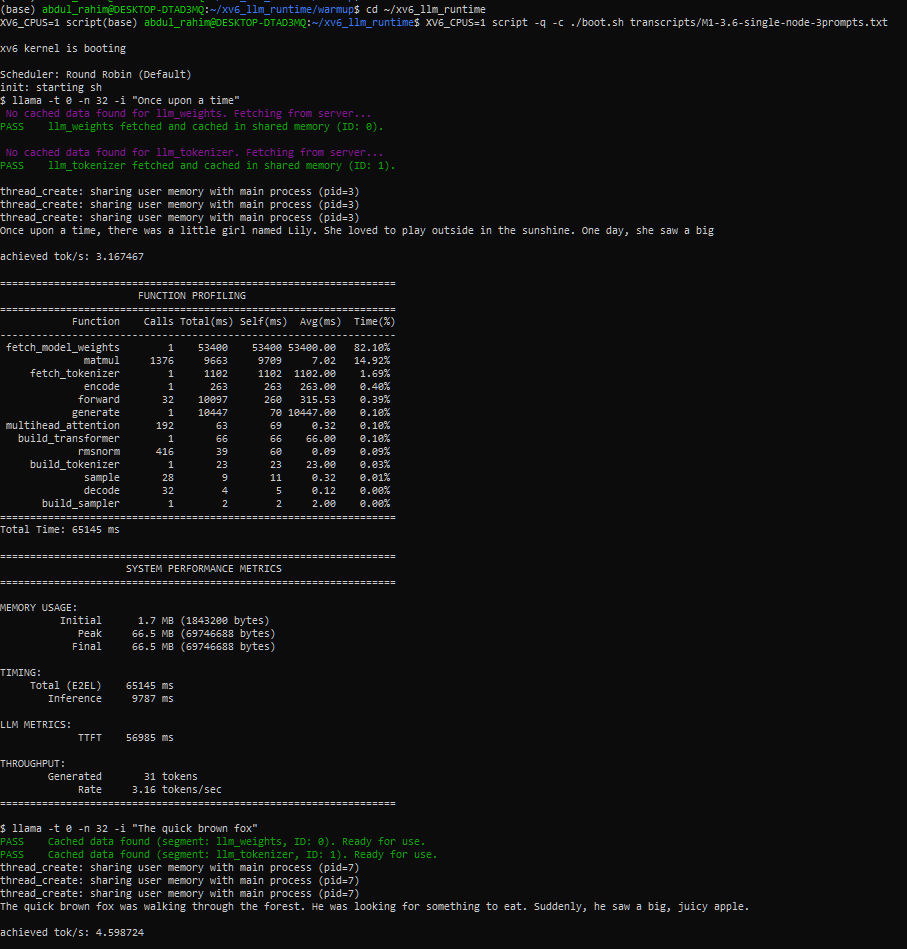
\includegraphics[height=0.52\textheight]{M1-3.6-01-single-node-prompt1.png}
\caption{Prompt 1, cold. \texttt{fetch\_model\_weights} is 82.1\% of elapsed time and the \texttt{Initial} memory reading is 1.7~MB.}
\label{fig:prompt1}
\end{figure}

\begin{figure}[H]
\centering
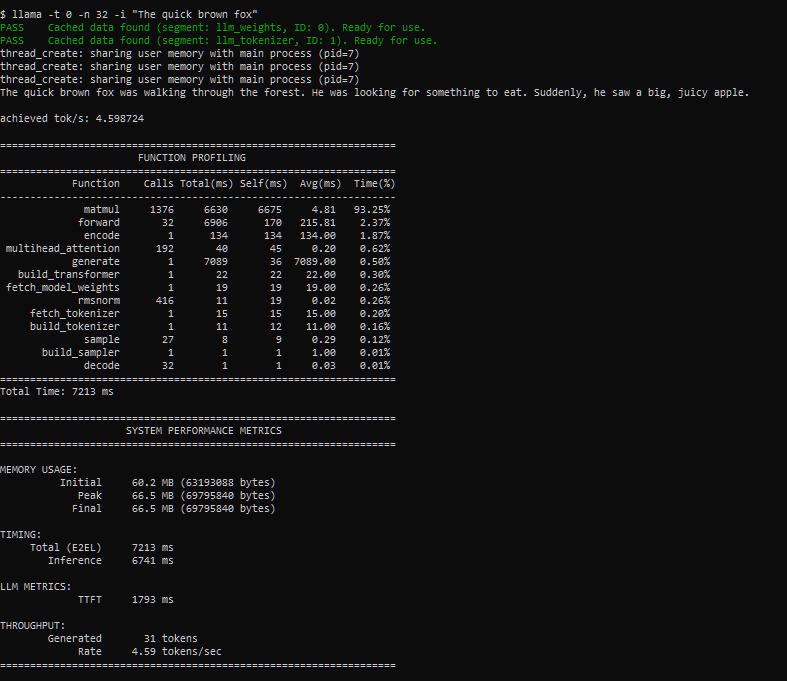
\includegraphics[height=0.52\textheight]{M1-3.6-02-single-node-prompt2.png}
\caption{Prompt 2, warm. No fetch occurs; \texttt{Initial} memory is 60.2~MB because the weights are already attached, and \texttt{matmul} is now 93.3\% of a much smaller total.}
\label{fig:prompt2}
\end{figure}

\begin{figure}[H]
\centering
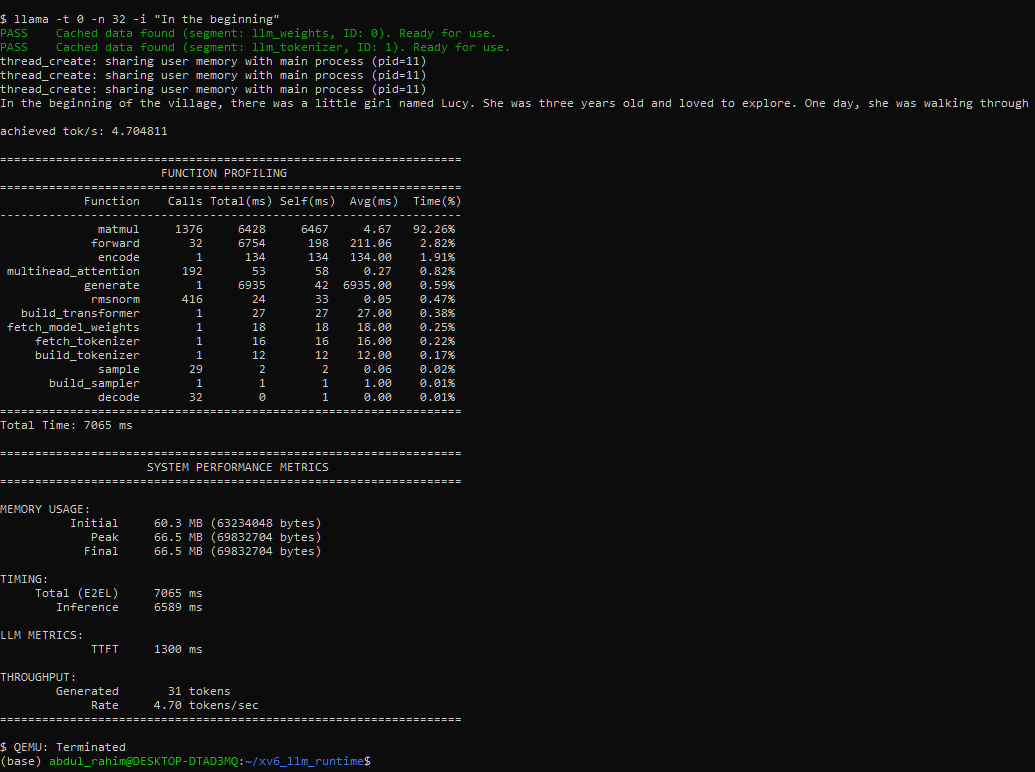
\includegraphics[height=0.52\textheight]{M1-3.6-03-single-node-prompt3.png}
\caption{Prompt 3, warm. Closely reproduces prompt 2, which is what makes that pair comparable and the cold run the outlier.}
\label{fig:prompt3}
\end{figure}

\paragraph{The first run in a boot is not comparable to the others.}
Its inference time is 45\% higher than the other two --- 9{,}787~ms against 6{,}741 and 6{,}589 --- despite performing identical work. The cause is not the weight fetch, which is accounted separately under TTFT. It is visible in the memory lines of Figures~\ref{fig:prompt1}--\ref{fig:prompt3}: the first run reports \texttt{Initial 1.7 MB} while the second and third report \texttt{Initial 60.2 MB}. On the first run the 60~MB of weights are paged in as \texttt{matmul} first touches them, inflating \texttt{matmul} from roughly 6{,}500~ms to 9{,}663~ms. Averaging all three prompts hides this; the mean is reported above for completeness, but the two warm runs are the comparable pair.

\subsection*{Ring, first prompt}

\begin{table}[H]
\centering
\small
\begin{tabular}{lrrrr}
\toprule
\textbf{Configuration} & \textbf{RTT/token ($\mu$s)} & \textbf{compute ($\mu$s)} & \textbf{network ($\mu$s)} & \textbf{tok/s} \\
\midrule
2 workers & 1{,}453{,}882 & 261{,}205 & 1{,}192{,}677 & 0.6 \\
3 workers & 2{,}943{,}042 & 393{,}747 & 2{,}549{,}295 & 0.3 \\
\bottomrule
\end{tabular}
\caption{Ring baseline on ``Once upon a time'', 32 steps, temperature 0, model \texttt{stories15M.bin}. Layer split: two workers \texttt{[0,3) [3,6)}; three workers \texttt{[0,2) [2,4) [4,6)}.}
\label{tab:baseline-ring}
\end{table}

\begin{figure}[H]
\centering
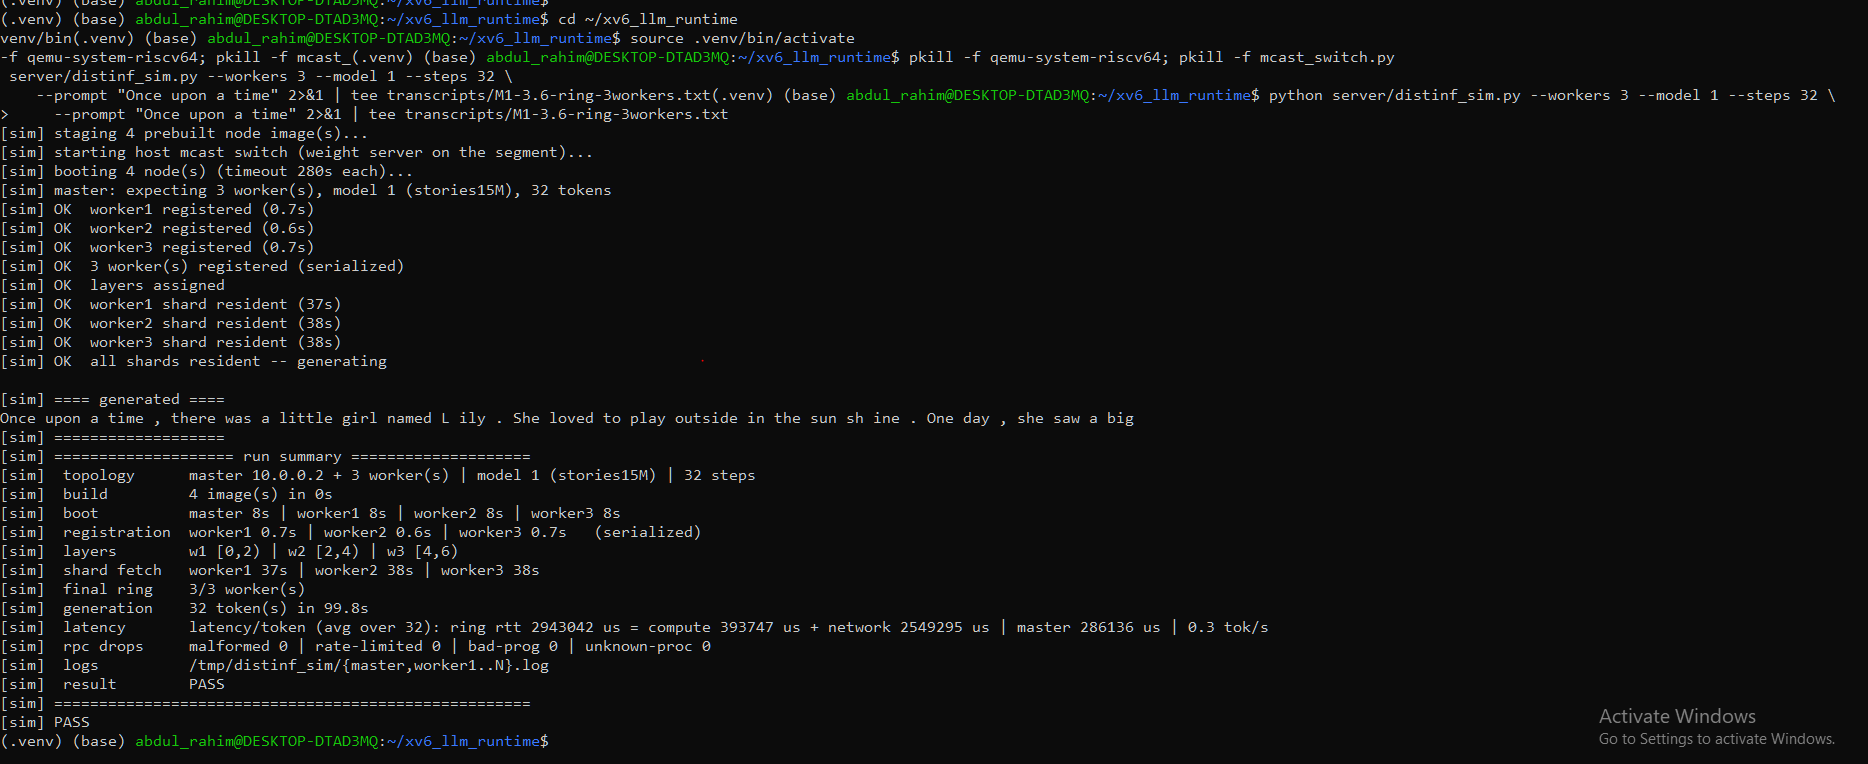
\includegraphics[width=0.98\textwidth]{M1-3.6-04-ring-3workers.png}
\caption{Three-worker ring. Layers split \texttt{[0,2) [2,4) [4,6)}, generation of 32 tokens took 99.8~s, and the latency line gives the compute/network split used in Table~\ref{tab:baseline-ring}.}
\label{fig:ring-3w}
\end{figure}

\subsection*{Analysis}

\textbf{Distribution costs more than it saves at this scale.} A single node generates at 4.7 tokens/second warm; two workers manage 0.6 and three manage 0.3. Adding the third worker halved throughput rather than improving it.

The mechanism is in the latency split. Network is 82.0\% of per-token round-trip time at two workers and 86.6\% at three. Total round-trip time doubled from 1.45~M to 2.94~M microseconds when the third worker was added, because each additional worker inserts another full network round trip into every token, while the six layers of work being divided are already small enough for one node to complete in about seven seconds. Pipeline parallelism pays only when per-stage compute time exceeds per-hop transport cost; here it is roughly a fifth of it.

Compute also rose, from 261{,}205 to 393{,}747 microseconds, even though the same six layers are computed either way. This is per-hop fixed overhead --- decode, validation, and the mailbox copy in \texttt{infer\_decode\_hop} --- multiplied by more hops.

\textbf{Core count matters more than node count here.} The same prompt at three cores on one node reached 5.97 tokens/second with \texttt{matmul} at 4{,}559~ms, against 3.16 tokens/second and 9{,}663~ms at one core: roughly a 2.1$\times$ speedup on \texttt{matmul} from the thread pool inside \texttt{multihead\_attention} (Figure~\ref{fig:F5}). Parallelism inside a node pays; parallelism across emulated nodes does not.

% =====================================================================
\section*{Section 3.7 --- Observations Log}
\addcontentsline{toc}{section}{Section 3.7 --- Observations Log}
% =====================================================================

Recorded while reading the shipped source and running the system. Nothing here was fixed. Several entries are design limits rather than defects and are marked as such.

\begin{enumerate}[leftmargin=1.4cm, itemsep=8pt]

\item \textbf{\texttt{user/discovery.h:116} --- a field named for milliseconds holds ticks.} The worker registry declares \texttt{uint32 last\_seen\_ms}, commented ``updated on each \texttt{PROC\_HEARTBEAT}''. The value assigned to it is in system ticks: the surrounding timing constants at \texttt{user/discovery.h:18--25} are all tick-denominated (\texttt{HEARTBEAT\_INTERVAL\_TICKS} 200, with \texttt{SUSPECTED\_TIMEOUT} and \texttt{EXPIRED\_TIMEOUT} derived from it). Any reader who takes the name at face value is out by a factor of the tick rate. This matches the calibration example given in the assignment.

\item \textbf{\texttt{user/discovery.h:101} --- the capability probe cannot prove what the threat model claims.} \texttt{CAP\_PROBE\_CEILING\_BYTES} is 32~MB, and the probe asks a candidate worker to back only \texttt{min(claim, ceiling)}. It can therefore establish ``has at least 32~MB'' and nothing more: a node with an ordinary budget that advertises 1~GB satisfies the probe effortlessly, and only a node whose real budget falls \emph{below} the ceiling is refused. The ceiling exists so that a claim cannot be turned into an unbounded allocation demand, so this is a limit on what a bounded probe can mean rather than a coding error --- but it is weaker than ``capability lying is closed by a sized probe'' suggests. The regression suite pins both sides of the boundary, including a case named \texttt{test\_capability\_lie\_above\_probe\_ceiling\_is\_accepted} (Figure~\ref{fig:distinf-regression}).

\item \textbf{\texttt{user/rpc.c:509--512} --- RPC retransmission has no backoff, and the code says so.} The comment reads: ``Per RFC 5531 \S5, we do not increase the timeout between retries here --- add exponential backoff if you observe QEMU congestion.'' Retries are issued at a fixed interval (\texttt{RPC\_MAX\_RETRIES} attempts of \texttt{RPC\_TIMEOUT\_MS} each, \texttt{user/rpc.c:482--483}). A simultaneous boot of many workers, or a master that drops and returns, produces synchronised fixed-interval retransmission across the whole segment.

\item \textbf{\texttt{kernel/syscall.h:74--80} --- a system-call numbering collision silently mis-dispatched five POSIX calls.} The header documents a real defect and its repair: the thread system calls were originally numbered 43--47, colliding with \texttt{setrlimit}, \texttt{getrlimit}, \texttt{capget}, \texttt{capdrop} and \texttt{getentropy}. Because \texttt{syscalls[]} is an array of designated initializers, a duplicate index is not a compile error --- the later initializer silently wins --- so all five POSIX calls were dispatching to thread and scheduler handlers. The failure mode is worth noting in its own right: the language offers no diagnostic for this class of mistake.

\item \textbf{\texttt{kernel/syscall.h} versus the binary --- 59 declared, 50 implemented.} Nine numbers (22--28, 33, 34) are declared with no handler symbol anywhere in the compiled kernel. \texttt{grep sys\_mmap kernel-symbols.txt} returns nothing while \texttt{grep sys\_setrlimit kernel-symbols.txt} returns \texttt{0x80001982}. The same pattern appears in \texttt{kernel/\allowbreak{}defs.h} for \texttt{stats.c}, \texttt{sprintf.c} and \texttt{vmcopyin.c}, all behind \texttt{\#ifdef} lab guards and likewise absent. See Section 3.5.

\item \textbf{\texttt{user/\allowbreak{}perf.c:260} --- the hardware counters are not wrapped by \texttt{perf.c}.} Only \texttt{rdtime} is: the line returns \texttt{(long long)(rdtime() / 10000)} and is the sole counter call in the file. \texttt{rdcycle()} and \texttt{rdinstret()} are declared at \texttt{user/\allowbreak{}user.h:39--41} and implemented in the kernel but have no caller in any \texttt{user/*.c} file, so instruction and cycle counts are unobtainable for a \texttt{llama} run without modifying code.

\end{enumerate}

\subsection*{Additional observations}

\begin{enumerate}[leftmargin=1.4cm, itemsep=8pt, start=7]

\item \textbf{\texttt{user/ftpclient.c:190, 547, 663, 695} --- each checkpoint's metadata is requested twice per fetch.} Observed live in the weight server log: \texttt{META\_RESP} is sent twice for file 1 and twice for file 2, both pairs at identical timestamps, and the shutdown statistics report \texttt{META\_REQs: 4} for a two-file transfer. \texttt{llm\_meta\_request} is defined at line 190 and called from three separate sites. The exact path is traced in Section 3.9.

\item \textbf{\texttt{user/llama.c:168, 361} --- \texttt{-n} counts steps, but the summary reports it as tokens generated.} \texttt{-n 32} yields \texttt{Generated 31 tokens}. The loop is \texttt{while (pos < steps)} --- 32 iterations --- but the first consumes the prompt token rather than emitting a new one. The flag is documented at line 361 as ``number of steps to run for'', which is accurate; the summary block's \texttt{Generated} label for the same quantity is not.

\item \textbf{The first inference in a boot is measurably slower than subsequent ones.} Across three prompts in one boot at \texttt{XV6\_CPUS=1}, the first run's inference took 9{,}787~ms against 6{,}741 and 6{,}589~ms for identical work, with the weight fetch excluded. The first run starts at \texttt{Initial 1.7 MB} and the later ones at \texttt{Initial 60.2 MB}, so the first pays the cost of paging in the 60~MB shared-memory segment as \texttt{matmul} first touches it. Any benchmark that averages the first run with later ones in the same boot is measuring two different things.


\item \textbf{\texttt{boot.sh}, \texttt{boot-gdb.sh} --- the RISC-V performance counters report host time, not guest instructions.} Neither script passes \texttt{-icount} to QEMU, so \texttt{\$instret} and \texttt{\$cycle} are both derived from the host's tick counter. Measured directly: over one \texttt{llama} run the \texttt{\$cycle} delta divided by that run's own reported elapsed time of 79.808~seconds is 3.289~GHz, the host's clock rate, and the absolute values correspond to the host's uptime rather than to time since the guest booted. Any number taken from these counters is a wall-clock measurement in disguise and the derived IPC is an artefact. This is a property of how the system is launched rather than a defect in the shipped code, but it determines what Section 3.6 can honestly claim, and it is the reason that section reports ratios rather than absolute counts.
\end{enumerate}

% =====================================================================
\section*{Section 3.8 --- Related Systems}
\addcontentsline{toc}{section}{Section 3.8 --- Related Systems}
% =====================================================================

\begingroup\small
\begin{longtable}{@{}R{0.18}R{0.41}R{0.41}@{}}
\toprule
\textbf{System} & \textbf{What it does that this system does not} & \textbf{What this system does that it does not} \\
\midrule
\endhead
Stock xv6 &
Maintains a minimalistic, teaching-focused kernel with a 21-syscall footprint and roughly 5,100 lines. That minimality is the pedagogical product, and every addition here erodes it. &
Adds 29 working system calls, a UDP/IPv4/ARP/ICMP stack with ingress and bogon filtering, shared memory, user-level threads, POSIX resource limits and capabilities, stack canaries with a real entropy source, W\^{}X at exec, and hardware performance counters. \\
\midrule
Linux &
Provides preemptive SMP scheduling, demand paging with swap, a complete TCP/IP suite, filesystem ownership and permissions, \texttt{mmap}, signals, namespaces and cgroups --- and mature implementations of the very primitives modelled here. &
Runs a transformer inference engine as ordinary user-space code on a kernel small enough to audit completely. Every syscall boundary the model crosses is visible and attributable; on Linux the same experiment is buried under millions of lines. \\
\midrule
xv6-llm-runtime-arch (upstream) &
Executes the transformer model entirely on a single node, so it carries none of the failure modes a network introduces: no registration, no heartbeats, no partial ring, no activation validation. &
Implements multi-node pipeline parallelism, a soft-state registry with authenticated registration and eviction, and network weight fetching over a custom transport. \\
\midrule
Exo &
Targets real heterogeneous consumer hardware --- phones, laptops, desktops --- with dynamic device discovery and partitioning across whatever is present, rather than a fixed ring of identical emulated nodes. &
Authenticates peers at registration and validates incoming tensors. The project README identifies Exo as the closest prior art and notes it has no authentication on peer discovery, no encryption, and no input validation on incoming tensors --- precisely the gaps this stack is built to close. \\
\midrule
Petals &
Runs 70B-class models across volunteer machines over the public internet, with fault tolerance and rebalancing at a scale this system does not approach, and supports fine-tuning as well as inference. &
Places peer trust inside the protocol. Petals' documented answer to untrusted participants is deployment-level: it advises running ``a private swarm among people you trust'' for sensitive data. This system instead requires PSK/HMAC identity at registration and a sized capability probe before a node is assigned a shard. \\
\midrule
Production Inference (vLLM) &
Uses PagedAttention for KV-cache management, continuous batching, speculative decoding, prefix caching, and both tensor and pipeline parallelism --- serving many concurrent users at production throughput on GPUs. &
Runs pipeline-parallel inference on a lightweight RISC-V teaching OS with no Python, no CUDA and no external libraries, and treats a lying participant as part of the threat model. vLLM assumes its workers are trusted infrastructure. \\
\bottomrule
\caption{Comparison against stock xv6, Linux, the upstream runtime architecture, and three distributed or production inference systems.}
\label{tab:related-systems}
\end{longtable}
\endgroup

\paragraph{Where this system sits.}
Measured purely as an inference engine it is far behind all three of the real systems above --- 4.7 tokens/second on one node, and worse when distributed (Section 3.6). Its contribution is not throughput. It is the only one of the six in which a distributed inference pipeline and the operating system underneath it are both small enough to be read completely, which is what makes an attack and its defence fully attributable to specific lines of code.

% =====================================================================
\section*{Section 3.9 --- Contributions (Bonus)}
\addcontentsline{toc}{section}{Section 3.9 --- Contributions (Bonus)}
% =====================================================================

\subsection*{1. Documentation Gap Closed \& Adoptable Figure}
\textbf{Proposal:} Replace the outdated hand-drawn \texttt{diagrams/state\_diagram.png} with the F3 Mermaid diagram (Figure~\ref{fig:F3}).

\textbf{Evidence:} The existing diagram actively misleads developers because it ignores the actual constants and states defined in \texttt{user/discovery.h}. It omits \texttt{PENDING}, the admission state in which a registered node must answer a sized capability probe before becoming \texttt{ACTIVE}, and it omits \texttt{SUSPECTED}, the recovery window between two and four missed heartbeats, modelling eviction instead as an immediate transition. The governing constants are \texttt{HEARTBEAT\_INTERVAL\_TICKS} 200, \texttt{HEARTBEAT\_MISS\_SUSPECTED} 2 and \texttt{HEARTBEAT\_MISS\_EXPIRED} 4, at \texttt{user/discovery.h:18--25}. A reader of the diagram would conclude that a worker missing two heartbeats is evicted; in the code it recovers. Because Mermaid is text-based, adopting the F3 diagram allows future contributors to version-control it and diff it against the constants it depicts --- the class of drift that produced this defect becomes visible rather than silent.

\subsection*{2. Real Defect: Every Whole-File Fetch Performs Two Metadata Round Trips}
\textbf{Proposal:} Split \texttt{llm\_fetch\_window} in \texttt{user/ftpclient.c} into a thin wrapper that fetches metadata and an inner routine that accepts already-fetched \texttt{file\_size} and \texttt{expected\_hash}.

\textbf{Evidence:} During a single-node bring-up the weight server logged \texttt{META\_RESP} twice for file 1 and twice for file 2, each pair at an identical timestamp, and its shutdown statistics reported \texttt{META\_REQs: 4} for a transfer of two files. Reading \texttt{user/ftpclient.c} explains it exactly. \texttt{llm\_fetch\_file} calls \texttt{llm\_meta\_request} at line 695 to learn \texttt{file\_size} so that it can \texttt{malloc} a destination buffer, then calls \texttt{llm\_fetch\_window(file\_id, buf, 0, file\_size, 0)} at line 705. \texttt{llm\_fetch\_window}, defined at line 537, opens with a comment reading \texttt{// Step 1: Request metadata} and issues a second, identical \texttt{llm\_meta\_request} at line 547. Neither call is conditional, so the duplication is unavoidable on this path.

Under the proposal, \texttt{llm\_fetch\_window} keeps its current signature and behaviour for existing callers, and \texttt{llm\_fetch\_file} calls the inner routine directly, passing the metadata it already holds. This removes one request/response pair per file with no protocol change and no change to any caller's semantics.

\subsection*{3. Real Defect: RPC Registration Storms}
\textbf{Proposal:} Implement randomised exponential backoff in \texttt{user/rpc.c}.

\textbf{Evidence:} The current RPC timeout mechanism does not implement exponential backoff, and the code says so explicitly at \texttt{user/rpc.c:509--512}: ``Per RFC 5531 \S5, we do not increase the timeout between retries here --- add exponential backoff if you observe QEMU congestion.'' If the master node drops offline and comes back, or a ring of ten or more workers boots simultaneously, every worker retransmits at the same fixed interval, synchronising traffic across the whole segment. Adding randomised exponential backoff would improve the distributed engine's network resilience. We note that the authors have already identified this gap; the contribution here is quantifying when it bites rather than discovering it.

\subsection*{4. Blocked Workflow: The Performance Counters Have No User-Space Caller}
\textbf{Proposal:} Extend \texttt{perf\_metrics} with \texttt{instret\_start}/\texttt{instret\_end} and \texttt{cycles\_start}/\texttt{cycles\_end}, sampled in \texttt{perf\_init()} and at the end of \texttt{generate()} (\texttt{user/\allowbreak{}llama.c:146,213}), and print both in the existing \texttt{SYSTEM PERFORMANCE METRICS} block.

\textbf{Evidence:} \texttt{rdcycle}, \texttt{rdtime} and \texttt{rdinstret} are implemented in the kernel (\texttt{sys\_rdcycle} \texttt{0x80001506}, \texttt{sys\_rdtime} \texttt{0x80001516}, \texttt{sys\_rdinstret} \texttt{0x80001526}) and declared at \texttt{user/\allowbreak{}user.h:39--41}. Only \texttt{rdtime} is ever called, at \texttt{user/\allowbreak{}perf.c:260}. Consequently instructions retired and cycles --- the metrics Section 3.6 is asked to report as primary --- cannot be obtained from the program's own output at all. Section 3.6 reports them by attaching a debugger and reading the CSRs directly, which works but is not reproducible from the runbook alone. The proposed change is roughly a dozen lines, uses only syscalls that already exist, and makes the measurement the assignment asks for reproducible without a code change in future milestones.

% =====================================================================
\section*{Appendices}
\addcontentsline{toc}{section}{Appendices}
% =====================================================================

\subsection*{Appendix A --- Transcripts (Bring-Up Evidence, Section 3.1)}

All three configuration transcripts required by Section 3.1 are reproduced in full in the Runbook (Section 3.2, Phase 2): the single-node run in Part A, the multi-node ring in Part B, and the weight-fetch path in Part C. Each is accompanied by the corresponding console screenshot --- Figures~\ref{fig:single-node}, \ref{fig:ring-2w} and \ref{fig:testftp} respectively. The kernel entry-point trace under GDB is in Section 3.0, Part E, with Figure~\ref{fig:gdb}.

\subsection*{Appendix B --- Evidence Index}

\begin{table}[H]
\centering
\small
\begin{tabular}{@{}lll@{}}
\toprule
\textbf{Screenshot} & \textbf{Shows} & \textbf{Referenced in} \\
\midrule
\texttt{M1-2.2-01-toolchain-versions}   & QEMU, objdump, GDB versions        & \S3.2 Phase 1 \\
\texttt{M1-2.4-01-checkpoints-verified} & Checkpoint sizes and digests       & \S3.2 Phase 1 \\
\texttt{M1-2.5-01-xv6-boot-and-ls}      & First boot, filesystem listing     & \S3.2 Phase 2 \\
\texttt{M1-2.6-01-weight-server-loaded} & Weight server ready                & \S3.2 Part A \\
\texttt{M1-2.6-02-single-node-generation} & Single-node run                  & \S3.2 Part A \\
\texttt{M1-2.7-01-ring-2workers}        & Two-worker ring, PASS              & \S3.2 Part B \\
\texttt{M1-3.1.3-01-testftp-bytes}      & Byte-exact weight fetch            & \S3.2 Part C \\
\texttt{M1-2.8-01-kernel-regression}    & 14 passed                          & \S3.2 Phase 3 \\
\texttt{M1-2.8-02-weightfetch-regression} & 4 passed                         & \S3.2 Phase 3 \\
\texttt{M1-2.8-03-distinf-regression}   & 2 passed, 6 skipped                & \S3.2 Phase 3 \\
\texttt{M1-2.9-01-kernel-symbols}       & Kernel symbol table                & \S3.2 Phase 4 \\
\texttt{M1-2.9-02-disas-sys-exec}       & Canary in the disassembly          & \S3.2 Phase 4, \S3.3 \\
\texttt{M1-2.10-01-gdb-sys-exec}        & Kernel entry-point trace           & \S3.0 Part E \\
\texttt{M1-3.0-01-nm-challenge}         & Warm-up symbol table               & \S3.0 Part A \\
\texttt{M1-3.0-02-disas-compute}        & \texttt{compute} disassembly       & \S3.0 Part B \\
\texttt{M1-3.0-03-all-jal-edges}        & All nine call sites                & \S3.0 Part B \\
\texttt{M1-3.6-01-single-node-prompt1}  & Baseline prompt 1 (cold)           & \S3.6 \\
\texttt{M1-3.6-02-single-node-prompt2}  & Baseline prompt 2 (warm)           & \S3.6 \\
\texttt{M1-3.6-03-single-node-prompt3}  & Baseline prompt 3 (warm)           & \S3.6 \\
\texttt{M1-3.6-04-ring-3workers}        & Three-worker ring                  & \S3.6 \\
\bottomrule
\end{tabular}
\caption{Index of console screenshots, all in \texttt{Screenshots/}.}
\label{tab:evidence-index}
\end{table}

\subsection*{Appendix C --- Commit Log}

Output of \texttt{git log --oneline} on \texttt{main} at the time of submission:

\begin{lstlisting}[style=shell]
ec052b0 (HEAD -> main, origin/main, origin/HEAD) Add Milestone 1 report
        figures and console screenshots
dd76f16 Initial commit: Milestone 1 starter
\end{lstlisting}

The repository holds the Milestone~1 handoff tree as received, together with the figure and screenshot sets referenced throughout this report (\texttt{Figures/} and \texttt{Screenshots/}). No file in the handoff was modified. That is deliberate and is what the short history records: Milestone~1 asks for the system to be measured exactly as distributed, so the baseline in Section 3.6 was taken against the unmodified tree and the hardware counters were read from outside the guest under a debugger rather than by adding instrumentation to \texttt{user/perf.c}. The change proposed in Section 3.9 is therefore stated as a proposal and is not present in this history.

\subsection*{Appendix D --- AI Use}

This report and parts of the work behind it were produced with assistance from a large language model. The assistance is declared in full below.

\begin{itemize}[leftmargin=1.4cm, itemsep=4pt]

\item \textbf{\LaTeX{} formatting.} Document structure, table and figure layout, and the diagnosis of compilation failures --- a font declaration misplaced inside a \texttt{longtable}, column widths that did not account for \texttt{\textbackslash tabcolsep}, a bare URL outside math mode, and a font-expansion error in \texttt{microtype}.

\item \textbf{Drafting and editing.} Prose for parts of several sections, written from measurements, transcripts and source that we produced ourselves, then reviewed and corrected by the team.

\item \textbf{Mermaid diagram sources.} The Mermaid source for figures F1--F7 was written with AI assistance. The content of each figure was specified by us from the source and the binary, and each rendered diagram was checked against the code it describes.

\item \textbf{Installation troubleshooting.} Toolchain and package errors on WSL2 Ubuntu, including the missing \texttt{python3-venv} package, \texttt{enumitem.sty} requiring \texttt{texlive-latex-extra}, and an incorrect QEMU package name (\texttt{qemu-system-riscv}, which does not exist in any Ubuntu release; the package that provides \texttt{qemu-system-riscv64} is \texttt{qemu-system-misc}).

\end{itemize}

All measurements, transcripts, screenshots and source-code locations reported here were produced by the team on our own machines. No figure, measurement or code reference in this report was taken from a model's output without being verified against the system itself.

\end{document}
